\documentclass[a4paper,fleqn]{cas-sc}

\usepackage[numbers]{natbib}
\usepackage{amsmath,amssymb}
\usepackage{booktabs}
\usepackage{longtable}
\usepackage{multirow}
\usepackage{subcaption}
\usepackage{float}
\usepackage{placeins}
\usepackage{stfloats}
\usepackage{caption}
\usepackage{tikz}
\usetikzlibrary{arrows.meta, positioning, shapes.geometric, calc}
\usetikzlibrary{positioning,arrows.meta,fit,backgrounds}
% ------------------------------------------------------------
% Float placement tuning
% ------------------------------------------------------------
% These settings make LaTeX more permissive with figure/table placement.
% They help reduce large blank spaces caused by restrictive float rules.
\renewcommand{\topfraction}{0.95}
\renewcommand{\bottomfraction}{0.85}
\renewcommand{\textfraction}{0.05}
\renewcommand{\floatpagefraction}{0.75}

\setcounter{topnumber}{5}
\setcounter{bottomnumber}{5}
\setcounter{totalnumber}{10}

% The numerical-display convention is stated once at the start of the Results.




\begin{document}

\let\WriteBookmarks\relax

\shorttitle{RMT-filtered networks: retrospective volatility assessment}
\shortauthors{A.V.S. Souza et al.}

\title[mode=title]{Random Matrix Filtering and Planar Financial Networks: A Retrospective Assessment for Volatility Forecasting in Complex Financial Markets}

\author[1]{Andrey V. S. Souza}[orcid=0009-0006-4177-758X]
\cormark[1]
\ead{andreyvinicius@furg.br}
\credit{Conceptualization, Methodology, Software, Formal analysis, Writing - original draft}

\author[1]{Bruno L. Dalmazo}[orcid=0000-0002-6996-7602]
\ead{dalmazo@furg.br}
\credit{Methodology, Supervision, Writing - review and editing}

\author[1]{Giancarlo Lucca}[orcid=0000-0002-3776-0260]
\ead{giancarlo.lucca@furg.br}
\credit{Methodology, Validation, Writing - review and editing}

\author[1]{Eduardo N. Borges}[orcid=0000-0003-1595-7676]
\ead{eduardoborges@furg.br}
\credit{Supervision, Methodology, Writing - review and editing}

\author[1]{Richard F. Pinto}[orcid=0009-0007-0176-3383]
\ead{richardpinto@furg.br}
\credit{Software, Data curation, Validation}

\author[2]{Fabian C. Cardoso}[orcid=0000-0002-2842-0387]
\ead{fabian@unirv.edu.br}
\credit{Data curation, Resources, Writing - review and editing}

\author[1]{Viviane L. D. de Mattos}[orcid=0000-0002-3512-6290]
\ead{vivianemattos@furg.br}
\credit{Formal analysis, Supervision, Writing - review and editing}

\author[1]{Rafael A. Berri}[orcid=0000-0002-3812-4186]
\ead{rafaelberri@furg.br}
\credit{Supervision, Project administration, Writing - review and editing}

\affiliation[1]{
  organization={Federal University of Rio Grande (FURG)},
  city={Rio Grande},
  state={Rio Grande do Sul},
  country={Brazil}
}

\affiliation[2]{
  organization={University of Rio Verde (UniRV)},
  city={Rio Verde},
  state={Goias},
  country={Brazil}
}

\cortext[cor1]{Corresponding author.}

\begin{abstract}
This study characterizes the dependency structure of Brazilian equities traded on B3 and retrospectively evaluates whether structural descriptors improve realized-volatility forecasts. The complete synchronized panel contains 58 equities over 1,527 dates from 23 August 2006 to 15 August 2024. Random Matrix Theory identifies four non-market eigenvalues above the Mar\v{c}enko--Pastur upper bound in the full panel and two after issuer collapse on the same dates. The leading eigenvalue accounts for 37.3\% of the full-panel correlation trace. Minimum Spanning Tree and Planar Maximally Filtered Graph analyses show that market-mode removal lowers edge correlations while preserving localized organization. In the validation-selected Ridge comparisons, adding market/RMT or network descriptors produces higher test QLIKE than Set A at both 5- and 20-day horizons; HAC tests favor the Set A baseline. These are retrospective comparisons because the structural descriptors use the full sample, and they do not establish a point-in-time forecasting benefit.
\end{abstract}

\begin{graphicalabstract}
\centering
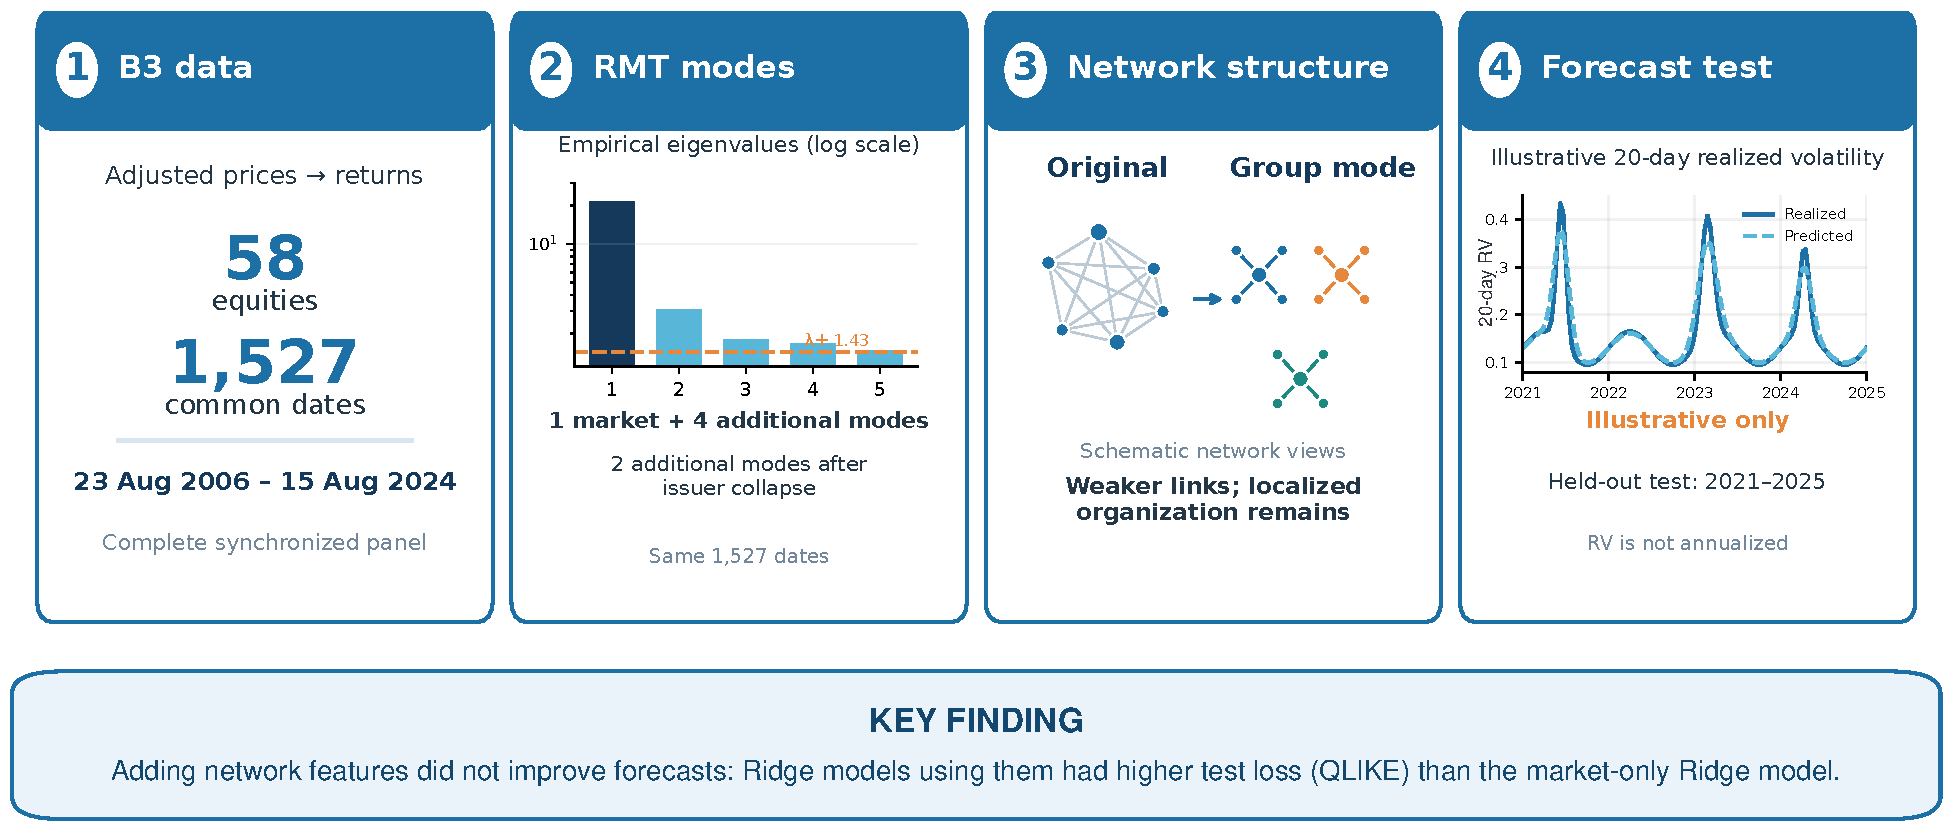
\includegraphics[
    width=\textwidth,
    keepaspectratio
]{images/graphical_abstract_vector_v7_o.pdf}
\end{graphicalabstract}

\begin{highlights}
\item Random-matrix spectra identify market, group and noise-compatible modes.
\item Planar filtering exposes localized sectoral dependency patterns.
\item Within-sector correlations exceed between-sector correlations on average.
\item Validation-selected Ridge Set B/C have higher test QLIKE than Set A.
\item Compact neural models extend the machine-learning comparison.
\end{highlights}

\begin{keywords}
Econophysics \sep Random matrix theory \sep Financial networks \sep
Planar maximally filtered graph \sep Volatility forecasting \sep
Machine learning \sep Brazilian stock market
\end{keywords}

\maketitle

\section{Introduction}
\label{sec:introduction}

Financial markets are often studied as complex systems where different investors, institutions, liquidity conditions, information flows, and feedback mechanisms interact over time \cite{mantegna_stanley_1999_book}. Although daily asset returns describe how individual prices change, they do not capture the full structure of the market \cite{cont_2001_empirical}. An important part of this structure comes from the relationships between assets, particularly how they move together. These relationships can be summarized through a correlation matrix, which may reflect broad market movements, more localized patterns among groups of assets, and variations caused by limited samples \cite{laloux_1999_noise}. Random Matrix Theory (RMT) provides a useful benchmark for distinguishing between correlations that may arise from random estimation effects and those that may contain meaningful structural information \cite{plerou_2002_random,bun_2017_cleaning}.

This distinction matters because financial risk depends not only on how much each asset fluctuates, but also on how assets move together. Portfolio diversification, contagion, and systemic risk are therefore strongly influenced by the correlation structure of the market \cite{billio_2012_econometric}. During relatively calm periods, correlations may remain moderate and heterogeneous. During periods of financial stress, however, assets often become more synchronized, reducing diversification benefits and concentrating market risk \cite{junior_2012_correlation,zheng_2012_changes}. Understanding this dependence structure therefore requires looking beyond individual return series and examining how collective and localized patterns emerge across the market.

The Brazilian equity market provides a useful setting for studying these dependency patterns. B3 \textit{(Brasil, Bolsa, Balcão)}, the country's main exchange and financial-market infrastructure provider\footnote{\url{https://www.b3.com.br/}}, includes companies from sectors such as finance, commodities, utilities, industry, consumer goods, real estate, and telecommunications. This diversity makes it possible to examine whether broad market synchronization coexists with more localized sectoral and group-level structures. Previous studies in Brazil have investigated interbank networks \cite{tabak_2010_topology}, multiscale correlations \cite{pereira_2019_multiscale}, agrarian cross-correlations \cite{stosic_2015_correlations}, and equity-market topology \cite{leonel_2022_brazilian}. Whether adding spectral and network descriptors improves volatility forecast accuracy in a broad B3 equity panel remains less examined.

To investigate this structure, we first use RMT to separate the dominant collective component of the market from smaller group-level components and from correlations compatible with sampling noise. This decomposition allows us to move beyond the raw correlation matrix and examine which dependency patterns remain after the broad market mode is removed. Rather than interpreting every significant eigenmode as a predefined economic sector, we use the spectral decomposition as an intermediate step for identifying and comparing market structure at different scales.

Once the broad market component is separated, the next question is how the remaining dependencies are organized across assets. We address this question through hierarchical and network representations of the original and RMT-filtered correlation structures. The Minimum Spanning Tree (MST) provides a sparse representation of the strongest dependency backbone \cite{mantegna_1999_hierarchical}, while the Planar Maximally Filtered Graph (PMFG) preserves a richer set of relationships and local connectivity patterns \cite{tumminello_2005_tool,tumminello_2010_correlation}. By comparing these representations before and after market-mode removal, we examine whether localized structures become more visible, whether central assets change, and whether sectoral or subsector-level organization persists beyond broad market synchronization.

Together, these steps form a single experimental sequence: the empirical dependence structure is first identified, then decomposed through spectral filtering, and finally examined through hierarchical and network representations. The resulting structural descriptors are subsequently evaluated in a retrospective volatility-model assessment.


The analysis combines these layers in the Brazilian equity-market context. The asset universe and network-construction rules are held fixed while the original correlation structure is compared with the dependencies that remain after removal of the dominant market mode. This design traces how spectral filtering relates to hierarchical organization, network topology, hub structure, and subsector connectivity. The final retrospective experiment tests whether adding the resulting structural descriptors improves volatility forecast accuracy; it does not establish a point-in-time forecasting benefit. The implementation, configuration files, and reproducibility documentation are available in the accompanying research-software repository \cite{rmt_planar_networks_2026}.

The paper makes four main contributions:
\begin{enumerate}
\item The dependency structure of B3 equities is characterized using adjusted daily prices with raw historical coverage from 1998 to 2025, combining stylized facts, cross-sectional correlations, sectoral comparisons, and time-varying market synchronization.

\item Random Matrix Theory is applied to a complete synchronized panel of 58 equities from 23 August 2006 to 15 August 2024, separating the dominant market component, candidate group-mode components, and noise-compatible variation in the empirical correlation matrix.

\item The hierarchical and network organization of the original and RMT-filtered dependency structures is compared, with particular attention to clustering, hub reorganization, sectoral retention, and subsector-level connectivity.

\item A chronological, nested-feature-set retrospective assessment tests whether adding full-sample RMT and network descriptors improves realized-volatility forecast accuracy. The structural features are not available at historical forecast origins, so this experiment does not establish a point-in-time forecasting benefit.
\end{enumerate}

The article is organized as follows. Section~\ref{sec:theoretical_background} presents the theoretical and conceptual foundations, while Section~\ref{sec:related_work} reviews the relevant literature and positions the proposed framework within previous work. Section~\ref{sec:methodology} describes the reproducible experimental framework. The results are then presented in Section~\ref{sec:results}, following an experimental sequence that ranges from the empirical dependency structure to robustness analysis and retrospective volatility assessment. The article concludes with a discussion of the findings, limitations, and directions for future point-in-time analyses.

\section{Theoretical Background and Conceptual Framework}
\label{sec:theoretical_background}

This section establishes the theoretical, mathematical and econophysics foundations of the research pipeline. We formalize cross-sectional financial dependencies and finite-sample estimation noise, Random Matrix Theory (RMT) spectral filtering, topological planar graphs (MST and PMFG), and the principles of realized volatility modeling in complex networks.

\subsection{Cross-Sectional Dependencies and Complex Market Dynamics}
\label{subsec:theory_market_dynamics}

Financial markets operate as complex interconnected systems where asset prices continuously interact through macroeconomic news, sector trends, liquidity cycles, and investor behavior \cite{mantegna_stanley_1999_book,bouchaud_potters_2003}. Rather than analyzing individual stocks in isolation, modern risk management focuses on understanding how assets move together across the entire market cross-section.

To compare price changes consistently across different companies, prices are converted into daily logarithmic returns:
\begin{equation}
r_{i,t} = \ln\left(\frac{P_{i,t}^{\mathrm{adj}}}{P_{i,t-1}^{\mathrm{adj}}}\right),
\label{eq:theory_log_returns}
\end{equation}
where $P_{i,t}^{\mathrm{adj}}$ is the dividend- and split-adjusted closing price of asset $i \in \{1, \dots, N\}$ on trading day $t \in \{1, \dots, T\}$ \cite{campbell_1997_econometrics,tsay_2005_analysis}. Across global stock markets, return series share several well-established universal behaviors, known as \emph{stylized facts} \cite{cont_2001_empirical}:
\begin{itemize}
  \item \textbf{Heavy Tails (Non-Gaussianity):} Extreme positive or negative price swings occur much more frequently than predicted by a standard normal curve (leptokurtosis) \cite{mandelbrot_1963_variation,fama_1965_behavior}.
  \item \textbf{Volatility Clustering:} While raw daily returns show little linear predictability, price volatility clusters in time---turbulent days are typically followed by turbulent days, and calm days by calm days \cite{engle_1982_autoregressive,bollerslev_1986_generalized}.
  \item \textbf{Asymmetric Co-movement:} Correlations between stocks tend to increase sharply during market downturns, which temporarily reduces the benefits of portfolio diversification \cite{longin_solnik_2001_extreme,ang_chen_2002_asymmetric}.
\end{itemize}

To measure co-movement without distortion from differences in individual asset volatility, each return series is normalized to zero mean and unit variance, $\widetilde{r}_{i,t} = (r_{i,t} - \widehat{\mu}_i)/\widehat{\sigma}_i$. The resulting standardized matrix $\widetilde{\mathbf{R}} \in \mathbb{R}^{T \times N}$ yields the Pearson cross-correlation matrix:
\begin{equation}
\mathbf{C} = \frac{1}{T-1} \widetilde{\mathbf{R}}^{\top} \widetilde{\mathbf{R}},
\label{eq:theory_corr_matrix}
\end{equation}
where each entry $C_{ij} \in [-1, 1]$ represents the pairwise linear correlation between assets $i$ and $j$.

However, a fundamental practical obstacle arises when the number of assets $N$ is comparable to the observation history $T$ (i.e., when $Q = T/N$ is finite). Under these conditions, sample correlation matrices become heavily contaminated by random sampling fluctuations, a phenomenon known as \emph{noise dressing} \cite{laloux_1999_noise}. Purely accidental historical coincidences can easily masquerade as real economic relationships. Directly relying on unfiltered sample correlations can severely distort portfolio optimization, network reconstruction, and risk forecasting, creating the need for principled filtering methods.

\subsection{Random Matrix Theory and Spectral Noise Filtering}
\label{subsec:theory_rmt}

Random Matrix Theory (RMT), originally introduced in mathematical physics to model the energy spectra of complex nuclei \cite{guhr_muller_1998}, provides an analytical benchmark to separate genuine economic structure from random sampling noise in empirical correlation matrices \cite{laloux_1999_noise,plerou_2002_random}.

Under the null hypothesis of a purely random Wishart ensemble, $\mathbf{X} \in \mathbb{R}^{T \times N}$ consists of mutually independent standard normal variables ($X_{ti} \sim \mathcal{N}(0, 1)$). In the asymptotic limit $N, T \to \infty$ with $Q = T/N \ge 1$, the eigenvalue density $\rho(\lambda) = \frac{1}{N}\sum_{k=1}^N \delta(\lambda - \lambda_k)$ of the sample covariance matrix $\mathbf{W} = \frac{1}{T}\mathbf{X}^{\top}\mathbf{X}$ converges almost surely to the Mar\v{c}enko--Pastur (MP) probability distribution \cite{marcenko_1967_distribution}:
\begin{equation}
\rho_{\mathrm{MP}}(\lambda) = \frac{Q}{2\pi \sigma^2 \lambda} \sqrt{(\lambda_+ - \lambda)(\lambda - \lambda_-)}, \quad \text{for } \lambda \in [\lambda_-, \lambda_+],
\label{eq:theory_marcenko_pastur}
\end{equation}
with theoretical support bounded by $\lambda_{\pm} = \sigma^2 \left(1 \pm \sqrt{1/Q}\right)^2$, where $\sigma^2$ is the residual variance parameter.

When evaluated against empirical financial correlation matrices, the eigenspectrum $\mathbf{C} = \sum_{k=1}^N \lambda_k \mathbf{v}_k \mathbf{v}_k^{\top}$ ($\lambda_1 \ge \lambda_2 \ge \dots \ge \lambda_N$) exhibits a characteristic tripartite decomposition \cite{plerou_2002_random,bun_2017_cleaning}:
\begin{enumerate}
  \item \textbf{Market Mode ($\lambda_1 \gg \lambda_+$):} The largest eigenvalue sharply exceeds the MP upper bound $\lambda_+$, absorbing a substantial fraction of the total matrix trace ($\operatorname{Tr}(\mathbf{C}) = N$). Its eigenvector $\mathbf{v}_1$ has strictly positive and relatively uniform loadings ($v_{1,i} \approx 1/\sqrt{N}$), representing pervasive macroeconomic co-movement that pulls all equities simultaneously.
  \item \textbf{Group Modes ($\lambda_k > \lambda_+$ for $k = 2, \dots, K_{\mathrm{signal}}$):} Intermediate eigenvalues that remain above $\lambda_+$ may reflect localized collective structure associated with industry groups, business conglomerates or shared factor exposures; their economic interpretation requires separate validation.
  \item \textbf{Bulk Noise Component ($\lambda_k \in [\lambda_-, \lambda_+]$):} The bulk of intermediate and small eigenvalues fall within the theoretical MP band, indicating sampling noise statistically indistinguishable from a random Wishart matrix.
\end{enumerate}

To isolate candidate localized dependencies from the dominant market mode and bulk noise, RMT enables spectral matrix reconstruction. Removing the dominant market mode ($k=1$) while retaining candidate group modes ($k = 2, \dots, K_{\mathrm{signal}}$) produces the group-mode filtered matrix:
\begin{equation}
\mathbf{C}_{\mathrm{group}} = \sum_{k=2}^{K_{\mathrm{signal}}} \lambda_k \mathbf{v}_k \mathbf{v}_k^{\top} + \overline{\lambda}_{\mathrm{rem}} \mathbf{I},
\label{eq:theory_c_group}
\end{equation}
where $\overline{\lambda}_{\mathrm{rem}} = \frac{1}{N - K_{\mathrm{signal}} + 1} \left( N - \lambda_1 - \sum_{k=2}^{K_{\mathrm{signal}}} \lambda_k \right)$ preserves the trace constraint, with diagonal elements subsequently normalized such that $(C_{\mathrm{group}})_{ii} = 1$.

\subsection{Topological Filtering and Planar Network Representations}
\label{subsec:theory_networks}

The correlation matrix records the relationship between every pair of assets. This complete representation is useful for calculation, but it is difficult to interpret because all assets are connected to one another. Even after RMT filtering removes noise-compatible components, the matrix does not directly show which dependencies form the market backbone, which assets behave as hubs, or whether sectoral groups remain visible. Topological filtering addresses this problem by retaining an informative subset of the strongest relationships and representing them as a network \cite{tumminello_2010_correlation}.

In this network, each asset is a node and each retained dependency is an edge. Correlations are first converted into distances using the transformation proposed by Mantegna \cite{mantegna_1999_hierarchical}: assets with stronger positive correlations are placed closer together, whereas weakly or negatively correlated assets are farther apart. This distance representation allows standard graph algorithms to select the most relevant connections. The network is therefore a simplified view of the correlation structure, not a replacement for the underlying matrix and not evidence of a causal relationship between companies.

In this study, networks are constructed from both the original correlation matrix and the RMT group-mode matrix. Comparing these representations shows which connections are mainly driven by the broad market movement and which localized structures remain after that common component is removed.

\subsubsection{Minimum Spanning Tree (MST)}
The Minimum Spanning Tree (MST) provides the sparsest connected representation of the market. It links every asset while preferentially retaining the shortest distances, and therefore the strongest correlations, without allowing closed loops \cite{mantegna_1999_hierarchical,bonanno_2004_networks}. The result can be read as a market backbone: branches indicate groups of closely related assets, central nodes indicate potential hubs, and peripheral nodes represent assets that are less integrated with the rest of the network.

The MST is useful because it makes the main dependency hierarchy easy to visualize. Its simplicity is also a limitation, since alternative routes and triangular relationships are discarded. We use the MST to compare the backbone obtained from the original correlations with the backbone that remains after market-mode removal, focusing on changes in hubs and sectoral organization.

\subsubsection{Planar Maximally Filtered Graph (PMFG)}
The Planar Maximally Filtered Graph (PMFG) retains more of the correlation structure than the MST. Connections are considered from strongest to weakest and are added while the graph can still be represented on a plane without edge crossings \cite{tumminello_2005_tool}. Unlike the MST, the PMFG allows loops and interconnected neighborhoods. It can therefore reveal local clusters, alternative dependency paths and groups of assets that share several strong relationships.

This richer structure is particularly useful for examining whether companies from the same sector remain connected, whether a small number of firms concentrate many relevant links, and how local organization changes after RMT filtering \cite{aste_2010_correlation,pozzi_2013_spread}. In this work, the PMFG complements the MST by supporting comparisons of clustering, sector retention, hub rankings and subsector-level dependencies. Detailed construction rules and mathematical properties are available in the original methodological references \cite{tumminello_2005_tool,tumminello_2010_correlation}.

\subsubsection{Network Descriptors Used in This Study}
Once the filtered networks are constructed, standard descriptors summarize the role of each asset and the organization of the market:
\begin{itemize}
  \item \textbf{Degree centrality} counts how many direct connections an asset has and helps identify highly connected hubs.
  \item \textbf{Betweenness centrality} indicates how often an asset lies between other assets, highlighting potential bridges between groups.
  \item \textbf{Closeness centrality} measures how near an asset is to the rest of the network through the available paths.
  \item \textbf{Eigenvector centrality} gives greater importance to assets connected to other influential assets.
  \item \textbf{Local clustering} measures how strongly an asset's neighbors are connected to one another and helps identify cohesive local groups.
\end{itemize}

These descriptors do not represent predictive signals by themselves. They summarize structural roles in the filtered market and allow the original and group-mode networks to be compared consistently. In the retrospective volatility experiment, selected descriptors are added to conventional return and volatility variables to test whether they improve forecast accuracy. Because the structural descriptors are estimated from the full synchronized sample, this comparison is ex post rather than a real-time forecasting strategy.

\subsection{Realized Volatility and Supervised Predictive Modeling}
\label{subsec:theory_volatility}

Volatility describes the intensity of price fluctuations, regardless of whether prices move upward or downward. A low-volatility period is relatively calm, whereas a high-volatility period contains larger and less stable price movements. This information is important for risk measurement, portfolio allocation and position sizing because two assets with similar average returns may expose investors to very different levels of uncertainty.

Future volatility is not known when a forecast is made. After the forecast horizon has passed, it can be approximated from the returns observed during that period. For a horizon of $h$ trading days, the realized-volatility proxy used as a forecasting target is
\begin{equation}
\mathrm{RV}_{i,t}^{(h)} = \sqrt{\sum_{\tau=1}^{h} r_{i,t+\tau}^{2}},
\label{eq:theory_rv}
\end{equation}
where the square root returns the measure to the scale of the returns; an annualization factor can be applied when comparisons across sampling frequencies require it. This ex-post measure is called \emph{realized volatility} \cite{andersen_2003_modeling}. In this study, the forecasting task is not to predict the direction of the next price movement. It is to estimate how much PETR4, VALE3 and BBDC4 are likely to fluctuate over the following 5 or 20 trading days.

A supervised model learns from historical examples that contain two parts: information available at a given date and the volatility subsequently observed over the forecast horizon. During training, the model learns how the predictors are associated with later volatility. It then applies the learned relationship to dates that were not used for model fitting.

The conventional predictors summarize recent returns and volatility persistence. Additional feature sets introduce broad market information, RMT descriptors and the MST/PMFG network descriptors discussed in Section~\ref{subsec:theory_networks}. The comparison includes a linear Ridge model \cite{hoerl_kennard_1970_ridge}, tree-based models such as Random Forest and gradient boosting \cite{breiman_2001_random,friedman_2001_greedy}, and simple neural models \cite{bucci_2020_realized,christensen_2022_realized}. These approaches differ in how they combine the predictors: the linear model provides a simple baseline, tree-based models can capture nonlinear interactions, and neural models provide a limited deep-learning comparison. The purpose is to test whether adding structural information improves volatility forecast accuracy, not to claim that one model represents the true dynamics of the market.

No single metric provides a complete assessment, so the models are compared using complementary measures. For $M$ evaluation dates, the mean absolute error (MAE) and root mean squared error (RMSE) are:
\begin{equation}
\mathrm{MAE}=\frac{1}{M}\sum_{t=1}^{M}\lvert y_t-\widehat{y}_t\rvert,
\qquad
\mathrm{RMSE}=\sqrt{\frac{1}{M}\sum_{t=1}^{M}(y_t-\widehat{y}_t)^2}.
\label{eq:theory_mae_rmse}
\end{equation}
MAE weights all absolute deviations equally, whereas RMSE gives greater weight to large errors. The out-of-sample coefficient of determination compares the model with a training-mean benchmark:
\begin{equation}
R_{\mathrm{OOS}}^2 = 1 - \frac{\sum_{t=1}^{M}(y_t-\widehat{y}_t)^2}{\sum_{t=1}^{M}(y_t-\overline{y}_{\mathrm{train}})^2}.
\label{eq:theory_oos_r2}
\end{equation}
For positive realized and predicted volatility proxies, the variance-form Gaussian quasi-likelihood loss (QLIKE) used in the computations is
\begin{equation}
\mathrm{QLIKE}(y,\widehat{y}) = \ln(\widehat{y}^{2})+\frac{y^{2}}{\widehat{y}^{2}},
\label{eq:theory_qlike}
\end{equation}
This is equivalent, up to a term that depends only on the realized proxy, to the ratio form of QLIKE; thus, model rankings on the same evaluation observations are unchanged. QLIKE remains informative when realized volatility is an imperfect proxy for latent market risk \cite{patton_2011_volatility}. Lower MAE, RMSE and QLIKE values indicate better forecasts, while a higher out-of-sample $R^2$ indicates a stronger improvement over the benchmark.

Model configurations and feature sets are chosen with the validation period and are then evaluated on a separate chronological test period. This separation reduces the risk of selecting a model simply because it fits the evaluation sample well. The exact target construction, temporal split, model settings and statistical comparisons are reported in the methodology and results sections.

A real-time forecast made on a particular date may use only information that was available up to that date. The return and volatility predictors satisfy this principle because they are calculated from past observations. However, the RMT and network descriptors used in this study were estimated from the complete synchronized sample. For an early date in the sample, those descriptors therefore summarize information that would not yet have been available.

Consequently, the experiment should be interpreted as a retrospective structural assessment. It compares forecast accuracy with and without full-sample structural features, but it does not establish that those features could improve forecasts in real time. A deployable forecasting experiment would need to reconstruct the RMT and network descriptors repeatedly, using only data available before each prediction date.

\section{Related work}
\label{sec:related_work}

This section locates the manuscript at the intersection of financial dependence, RMT, filtered networks and volatility modelling. It distinguishes established tools from the contribution of the present study: an integrated B3 workflow and a clearly retrospective assessment of whether full-sample structural descriptors are associated with volatility-model performance.

\subsection{Financial dependencies and econophysics}

Econophysics studies financial markets using concepts and methods from statistical physics, nonlinear dynamics, complex systems and network science \cite{smolyak_havlin_2022_econophysics,vogl_2022_financial_chaos}. A central observation is that financial returns exhibit stylized facts that are difficult to reconcile with independent Gaussian models. Heavy tails, volatility clustering, slow decay in absolute-return autocorrelations, intermittent bursts of activity and collective co-movement patterns are recurrent findings across asset classes, countries and sampling frequencies \cite{mantegna_stanley_1999_book,cont_2001_empirical}. These regularities motivate methods that focus not only on the marginal distribution of returns, but also on dependency, synchronization and network structure.

Financial dependency analysis lies at the intersection of econophysics and financial economics. In financial economics, dependence is central to portfolio risk, diversification, contagion, factor structure and systemic vulnerability. In econophysics, the same dependence is often represented through correlation matrices, eigenspectra, filtered graphs and hierarchical structures. Network-based studies of stock markets have used this representation to connect correlation structure with market organization and temporal evolution \cite{chi_2010_network,kumar_2012_correlation}. Raddant and Di~Matteo \cite{raddant_dimatteo_2023} emphasize that correlations, causality measures, volatility spillovers and networks offer additional views of financial systems. We follow this perspective: the goal is not merely to estimate pairwise correlations, but to decompose the correlation matrix, filter its noisy components, represent the remaining structure as networks and evaluate whether the extracted network structure has forecasting relevance.

Cross-correlation dynamics during crises have received attention because market stress often increases synchronization across assets. Zheng et~al. \cite{zheng_2012_changes} showed that changes in cross-correlation structure can serve as early indicators of systemic instability. Billio et~al. \cite{billio_2012_econometric} proposed econometric measures of connectedness and systemic risk in financial sectors. Junior and Franca \cite{junior_2012_correlation} documented that correlations among global stock indices tend to increase during crises, reducing the effective dimensionality of international markets. These findings motivate the rolling-correlation and crisis-synchronization analysis undertaken in this paper, where market-wide co-movement is treated as an object of study instead of a nuisance.

The relevance of these studies for the present manuscript is twofold. First, they show that financial dependence is dynamic and crisis-sensitive. Second, they indicate that a single unfiltered correlation matrix may conceal different layers of structure: a broad market component, group or sectoral organization and residual noise. This motivates the use of Random Matrix Theory and filtered networks as additional tools for separating and interpreting these layers.

\subsection{Random Matrix Theory in financial correlations}

RMT-based finance was established as an empirical programme for deciding which parts of a large correlation matrix are reproducible rather than as a new asset-pricing theory. Laloux et~al. \cite{laloux_1999_noise,laloux_2000_random} reported that most eigenvalues of equity correlation matrices are compatible with a random benchmark and showed that removing this component can improve portfolio construction. Plerou et~al. \cite{plerou_2002_random} added an interpretation of the outlying eigenvectors: the leading one is a broad market mode, whereas some subleading modes are associated with sectors or other collective groups. These findings made spectral structure an empirical object in its own right, but they do not imply that every eigenvalue outside the random band has a unique economic meaning.

The methodological literature subsequently focused on how aggressively the noisy component should be treated. Bun et~al. \cite{bun_2017_cleaning} review eigenvalue clipping, shrinkage and rotationally invariant estimators, and stress that the choice of cleaning rule affects both the stability of the estimated covariance matrix and its downstream use. The broader mathematical foundations are reviewed by Guhr et~al. \cite{guhr_muller_1998}. Thus, RMT studies differ in their objective: some seek a portfolio-optimal covariance estimator, while others use eigenvectors to identify collective market factors.

Our use is narrower and explicitly comparative. We use the Mar\v{c}enko--Pastur edge to organize the empirical spectrum, remove the dominant market mode, retain candidate group-mode components and preserve the remaining trace in a residual component. The resulting matrix is not presented as an optimal covariance estimator. It is one controlled input to the paired MST/PMFG comparison, allowing us to ask whether localized topology changes after the common market component is removed. Because the decomposition is estimated from the complete synchronized panel, the comparison is retrospective.

\subsection{Financial networks: MST, PMFG and filtered graphs}

Mantegna's introduction of the MST made it possible to study market organization without imposing a fixed correlation threshold \cite{mantegna_1999_hierarchical}. Subsequent applications used the tree to describe sectoral and geographical taxonomies, portfolio organization and time-varying market integration. Onnela et~al. \cite{onnela_2003_dynamics} documented the evolution of market correlations and the changing concentration of the tree, while Bonanno et~al. \cite{bonanno_2004_networks} and Song et~al. \cite{song_2012_evolution} showed that the resulting hierarchies depend on both sector and market regime. The common result is interpretability, accompanied by a loss of cycles and alternative routes.

The PMFG line of work addresses that loss of local structure. Tumminello et~al. \cite{tumminello_2005_tool,tumminello_2010_correlation} used planar filtering to retain stronger links together with triangular relationships, making clustering and clique structure available for financial interpretation. Massara et~al. \cite{massara_2016_tmfg} proposed the TMFG as a related scalable construction for larger systems, while temporal-network formulations retain information about the evolution of market links \cite{zhao_2018_stock}. Other studies connected filtered topology to economic questions: Pozzi et~al. \cite{pozzi_2013_spread} related peripheral positions to diversification, Aste et~al. \cite{aste_2010_correlation} examined network changes in volatile periods, and Kenett et~al. \cite{kenett_2012_dominating} used partial correlations to distinguish direct from market-mediated links.

Many studies examine spectral filtering or network topology separately. This study constructs matched MST and PMFG representations before and after market-mode removal, holds the asset universe and ranking procedure fixed, and compares centrality, clustering and sector retention. This design uses topology to describe how spectral filtering changes the dependency representation; it does not treat the resulting links as causal.


Evidence from emerging markets shows why results from large developed-market datasets cannot simply be transferred to B3. Institutional structure, sector concentration, liquidity and exposure to commodities or exchange rates can alter both the level and the persistence of cross-sectional dependence. Existing work also uses several different network objects. Tabak et~al. \cite{tabak_2010_topology} studied the Brazilian interbank network and its vulnerability to targeted failures, while Silva et~al. \cite{silva_2016_structure} examined the position and dynamics of emerging economies in the global financial network. Wang et~al. \cite{wang_2018_correlation} compared Pearson and partial-correlation networks across world markets and found that the inferred structure depends on the dependence measure.

Studies closer to the equity-market setting remain fragmented. Pereira et~al. \cite{pereira_2019_multiscale} used detrended cross-correlation networks for a set of stock markets that includes Brazil; Ferreira et~al. \cite{ferreira_2019_detrended} compared detrended dependencies between oil and stock markets; Leonel Caetano and Yoneyama \cite{leonel_2022_brazilian} analysed the Brazilian stock market with complex-network measures; and Stosi{\'c} et~al. \cite{stosic_2015_correlations} focused on Brazilian agrarian commodities and stocks. These contributions establish that Brazilian data contain nontrivial multiscale and network structure, but they do not jointly evaluate a broad B3 equity universe, RMT group-mode filtering, planar graphs and volatility forecasting.

Our contribution is therefore contextual rather than a claim that B3 is representative of all emerging markets. We use the original and RMT-filtered networks to separate broad market integration from more localized organization, and we report the comparison descriptively. The subsequent volatility exercise asks whether these ex-post structural differences are associated with model performance; it does not infer a universal emerging-market mechanism or a tradable signal.

\subsection{Volatility forecasting and machine learning}

The forecasting literature provides two relevant benchmarks. Andersen et~al. \cite{andersen_2003_modeling} established the empirical role of realized volatility, while Poon and Granger \cite{poon_granger_2003} reviewed the comparative performance of volatility models. The HAR formulation of Corsi \cite{corsi_2009_simple} gives a transparent multi-horizon benchmark. Hansen and Lunde \cite{hansen_lunde_2005} explicitly compared a broad set of parametric volatility models, including GARCH(1,1), illustrating why new specifications should be evaluated against strong conventional benchmarks. These studies motivate the use of conventional return and volatility predictors as the baseline rather than treating a flexible learner as the default.

Machine-learning work has expanded the feature space and the class of admissible nonlinearities. Bucci \cite{bucci_2020_realized} used neural networks for realized-volatility forecasting, and Christensen et~al. \cite{christensen_2022_realized} developed a broader machine-learning framework. Random forests, boosting and regularized linear models remain useful comparison points because they expose different bias--variance and interpretability trade-offs \cite{breiman_2001_random,friedman_2001_greedy,hoerl_kennard_1970_ridge}.

Two methodological issues are central in this literature. First, realized volatility is a noisy proxy for latent variance, so Patton \cite{patton_2011_volatility} recommends loss functions such as QLIKE that are robust to measurement error. Second, flexible models can produce spurious improvements when temporal ordering, feature selection or the information set is not respected. Our experiment addresses these issues with a chronological train--validation--test split, complementary losses and nested feature sets. The network variables are treated as an incremental structural augmentation: because Sets~B and~C use full-sample RMT and network descriptors, their results are interpreted as retrospective associations, not point-in-time forecast gains.

\section{Methods: Integrated Empirical Framework}
\label{sec:methodology}

This section describes the empirical sequence: (i) B3 data and asset-universe construction, (ii) spectral separation of market, group and noise components, (iii) matched topological representations of original and filtered dependencies, and (iv) retrospective model assessment. The sequence can be reapplied to another market or sample by replacing the data and asset labels while preserving the stated decision rules. Figure~\ref{fig:methodology_overview} summarizes the analysis.

\begin{center}
\resizebox{0.94\linewidth}{!}{%
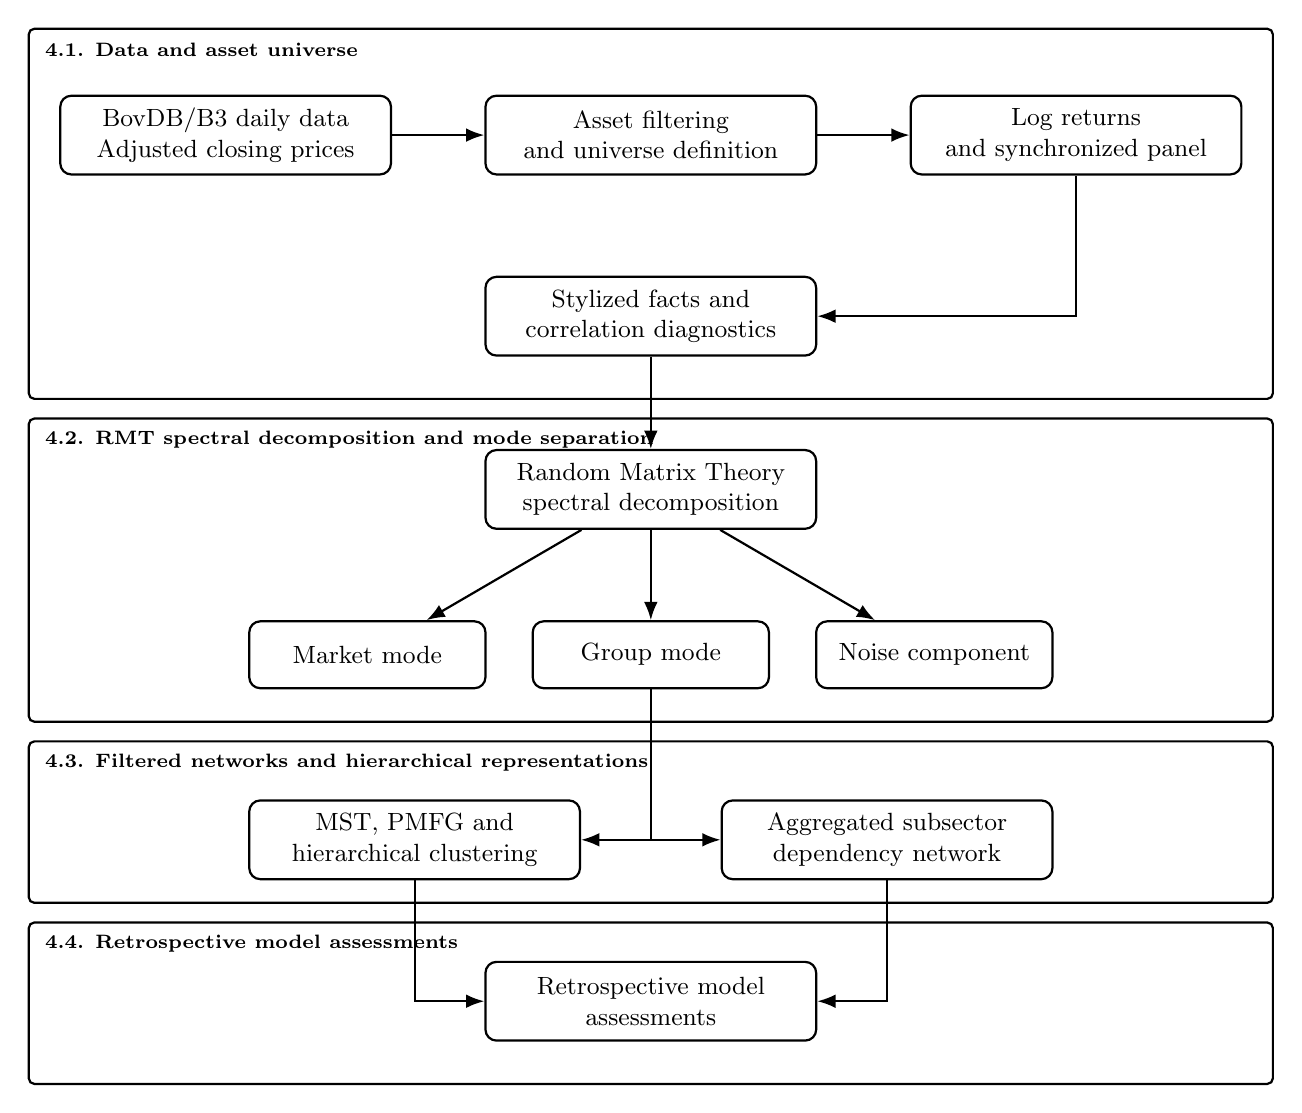
\begin{tikzpicture}[
    x=1cm, y=1cm, >=Latex,
    box/.style={rectangle,rounded corners,draw=black,thick,align=center,minimum width=4.2cm,minimum height=1.0cm,font=\small},
    smallbox/.style={rectangle,rounded corners,draw=black,thick,align=center,minimum width=3.0cm,minimum height=0.85cm,font=\small},
    sectionbox/.style={rectangle,rounded corners=2pt,draw=black,thick,fill=none},
    sectionlabel/.style={font=\bfseries\scriptsize,anchor=west,inner sep=0pt},
    line/.style={->,thick}]
% Section 4.1: data and asset universe
\draw[sectionbox] (-2.5,1.35) rectangle (13.3,-3.35);
% Section 4.2: RMT spectral decomposition and mode separation
\draw[sectionbox] (-2.5,-3.60) rectangle (13.3,-7.45);
% Section 4.3: filtered networks and hierarchical representations
\draw[sectionbox] (-2.5,-7.70) rectangle (13.3,-9.75);
% Section 4.4: retrospective model assessments
\draw[sectionbox] (-2.5,-10.00) rectangle (13.3,-12.05);
\node[box] (data) at (0,0) {BovDB/B3 daily data\\Adjusted closing prices};
\node[box] (filters) at (5.4,0) {Asset filtering\\and universe definition};
\node[box] (returns) at (10.8,0) {Log returns\\and synchronized panel};
\node[box] (diagnostics) at (5.4,-2.3) {Stylized facts and\\correlation diagnostics};
\node[box] (rmt) at (5.4,-4.5) {Random Matrix Theory\\spectral decomposition};
\node[smallbox] (market) at (1.8,-6.6) {Market mode};
\node[smallbox] (group) at (5.4,-6.6) {Group mode};
\node[smallbox] (noise) at (9.0,-6.6) {Noise component};
\node[box] (networks) at (2.4,-8.95) {MST, PMFG and\\hierarchical clustering};
\node[box] (aggregate) at (8.4,-8.95) {Aggregated subsector\\dependency network};
\node[box] (assessment) at (5.4,-11.0) {Retrospective model\\assessments};
\draw[line] (data)--(filters); \draw[line] (filters)--(returns);
\draw[line] (returns.south)|-(diagnostics.east); \draw[line] (diagnostics)--(rmt);
\draw[line] (rmt)--(market); \draw[line] (rmt)--(group); \draw[line] (rmt)--(noise);
% The group-mode matrix feeds the two matched network representations.
\draw[thick] (group.south) -- (5.4,-8.95);
\draw[line] (5.4,-8.95) -- (networks.east);
\draw[line] (5.4,-8.95) -- (aggregate.west);
% Both network outputs feed the retrospective model assessments.
\draw[line] (networks.south)|-(assessment.west);
\draw[line] (aggregate.south) |- (assessment.east);
% Section labels are drawn last so connector lines cannot cross their text
\node[sectionlabel] at (-2.3,1.08) {4.1. Data and asset universe};
\node[sectionlabel] at (-2.3,-3.87) {4.2. RMT spectral decomposition and mode separation};
\node[sectionlabel] at (-2.3,-7.97) {4.3. Filtered networks and hierarchical representations};
\node[sectionlabel] at (-2.3,-10.27) {4.4. Retrospective model assessments};
\end{tikzpicture}%
}
\captionof{figure}{Overview of the workflow. The workflow proceeds through stylized-fact checks, correlation estimation, Random Matrix Theory filtering, hierarchical clustering, MST/PMFG network construction, subsector aggregation and volatility forecasting with machine-learning, deep-learning, RMT and network-based features.}
\label{fig:methodology_overview}
\end{center}

\subsection{Data and asset universe}
\label{subsec:data_universe}

This first block defines the empirical universe before any dependence is estimated. It separates raw historical coverage, the complete panel required by spectral methods and the smaller set of representative assets used for the volatility experiment.

\label{subsec:bovdb_prices}

We use daily adjusted B3 equity prices from the locally held historical extraction and cite the public BovDB and BovDBv2 datasets for their documented source and coverage \cite{cardoso_2022_bovdb,souza_2024_bovdbv2}. Harvard Dataverse identifies BovDBv2 V1 as CC0 1.0 and records public daily/intraday coverage through 31 July 2024. The local extraction used here extends through 30 December 2025; the additional local records are not part of that public release, are not included in this package, and their source-specific redistribution terms have not been verified. Reproduction of the local extension therefore requires an authorized source and applicable access rights. We retain adjusted closing prices because corporate-action adjustments affect returns, correlations and graph weights.

\label{subsec:asset_filtering}

We apply deterministic filters to retain direct listed equities with valid, strictly positive adjusted prices. BDRs, ETFs, investment funds, indices and other non-equity vehicles are excluded. We inspect extreme adjusted-return observations as a quality-control step and remove an asset only when the evidence indicates an implausible corporate-action or ticker-history inconsistency. A minimum historical-coverage rule is then applied, one share class per issuer is retained where necessary, and the remaining assets are synchronized on common trading dates.

The resulting core historical universe contains 58 equities. Its raw unbalanced file spans 17 March 1998 to 30 December 2025, whereas the complete synchronized panel used for RMT, clustering and networks contains $N=58$ assets and $T=1527$ common observations from 23 August 2006 to 15 August 2024. The distinction prevents pairwise descriptive samples from being confused with the common panel required by the spectral analysis.

The universe is historical rather than restricted to currently listed firms. This preserves a long B3 cross-section while keeping the number of assets compatible with interpretable spectral and network visualizations. Table~\ref{tab:universe_summary} distinguishes the broader representative-asset coverage from the complete synchronized panel used for RMT, clustering and network construction.

\begin{center}
\captionof{table}{Summary of the samples used in this study.}
\label{tab:universe_summary}
\resizebox{\linewidth}{!}{%
\begin{tabular}{lrrl}
\toprule
Sample & Assets & Period & Main use \\
\midrule
Representative assets & 3 & 2006--2025 & Stylized facts and initial forecasting experiment \\
Core historical universe & 58 & 2006-08-23--2024-08-15 & RMT, clustering and networks (complete panel) \\
\bottomrule
\end{tabular}}
\end{center}

The complete-case restriction is important because the empirical correlation matrix must be estimated from a common set of trading dates across all assets. Static pairwise and rolling correlations may use the observations available for each pair or window; they therefore retain broader unbalanced coverage and should not be interpreted as estimates from the complete RMT panel.

Each asset in the core universe is assigned to a macro-sector, subsector and segment classification. The macro sectors include Financials, Oil Gas and Biofuels, Basic Materials, Utilities, Industrials, Consumer Cyclical, Consumer Non-Cyclical, Real Estate and Telecommunications. These labels are used for sectoral correlation comparisons, heatmap interpretation, sector-retention checks and subsector-level aggregation. Utilities and Real Estate are kept separate as a descriptive classification, not as a claim that all firms in either group share the same risk profile. Within Basic Materials, the subsector map distinguishes Mining, Steel and Metallurgy, Chemicals, and Paper and Cellulose; detailed asset assignments are provided in the supplementary material.

\label{subsec:notation}

Daily log returns follow the definition in Section~\ref{subsec:theory_market_dynamics}, Eq.~\eqref{eq:theory_log_returns}, and are applied to the adjusted closing-price series retained after filtering. The resulting synchronized return panel contains the same $N=58$ assets on the $T=1527$ common dates. Complete-case synchronization is performed before any dependence estimation so that eigenvalues, eigenvectors, distances and network edges refer to one fixed date--asset panel.

The main quality concern is the distinction between genuine extreme returns and artificial jumps caused by corporate-action adjustment problems. Adjusted prices reduce the impact of splits, dividends and related events, but do not guarantee that every historical corporate action, ticker transition, share-class change or reorganization is perfectly corrected. Extreme-return validation is therefore treated as a separate quality-control step, and assets with implausible corporate-action-related jumps are excluded from the main analyses. The complete synchronized panel provides a consistent input for RMT and networks but shortens the available historical window; results may differ under intraday sampling, alternative liquidity filters, rolling universes or broader forecasting targets.

\label{subsec:stylized_method}

The stylized-fact interpretation and standardization conventions are those defined in Section~\ref{subsec:theory_market_dynamics}. PETR4, VALE3 and BBDC4 are used as liquid, economically distinct demonstration assets for return diagnostics and as initial forecasting targets. We report return distributions, tail summaries, moments, empirical Value at Risk and autocorrelations of absolute returns. The Pearson correlation matrix is constructed according to Eq.~\eqref{eq:theory_corr_matrix}; this subsection specifies only its empirical use. Within- versus between-sector correlations are compared using the B3 classifications and an asset-level sector-label permutation check. Rolling average pairwise correlation is used as a descriptive synchronization measure. These diagnostics establish the empirical object passed to the spectral and network stages; they are not treated as trading signals or causal tests.

\subsection{RMT spectral decomposition and mode separation}
\label{subsec:rmt_method}

The spectral step follows the RMT formulation in Section~\ref{subsec:theory_rmt}, including the Mar\v{c}enko--Pastur density and support in Eq.~\eqref{eq:theory_marcenko_pastur} and the trace-preserving group-mode reconstruction in Eq.~\eqref{eq:theory_c_group}. Operationally, we apply that rule to the complete synchronized correlation matrix, order the eigenvalues from largest to smallest, remove the leading market mode, retain subsequent eigenmodes whose eigenvalues exceed the upper MP edge as candidate group components, and represent the remaining components by the residual term. The reconstructed matrix is normalized as a correlation matrix before network construction. This is a filtering convention rather than a claim that the MP null fully describes the Brazilian market; the term group mode denotes a spectral component, not a unique causal factor. Issuer-collapsed and circular-shift analyses are used as robustness checks for this descriptive interpretation.

\subsection{Filtered networks and hierarchical representations}
\label{subsec:network_method}

The same distance transformation and edge-ranking procedure is applied to the original correlation matrix and to the RMT group-mode matrix. This matched construction is central to the proposed methodology: differences in topology can then be attributed to the spectral input rather than to a change in the asset universe or graph algorithm.

\subsubsection{MST, PMFG and hierarchical clustering}
\label{subsec:distance_clustering_method}

We use the Mantegna distance $d_{ij}=\sqrt{2(1-C_{ij})}$, average-linkage clustering and ordered heatmaps to inspect hierarchical organization. The MST provides the sparse market backbone, while the PMFG retains additional planar links and local clustering. For each representation we compare degree, betweenness, closeness, eigenvector centrality and local clustering, together with sector retention and hub reorganization. The mathematical definitions of these standard descriptors are given in Section~\ref{subsec:theory_networks}; here they are operationalized as outputs of the paired original/group-mode construction. Cophenetic agreement is reported using the standard dendrogram-comparison perspective of Sokal and Rohlf \cite{sokal_rohlf_1962}.

\label{subsec:subsector_network_method}

Following the parallel MST/PMFG and hierarchical-clustering views, ticker-level dependency information is summarized as a mesoscopic economic representation. Retained ticker-level edges are assigned to pairs of B3 subsectors. For subsectors $a$ and $b$, the displayed weight is the mean retained dependency,
\begin{equation}
W_{ab}=\frac{1}{|\mathcal{E}_{ab}|}\sum_{(i,j)\in\mathcal{E}_{ab}}w_{ij},
\qquad \mathcal{E}_{ab}=\{(i,j)\in E:g(i)=a,\ g(j)=b\}.
\end{equation}
This operation compresses many asset-level links into an interpretable subsector-to-subsector map. It is used to identify whether filtered dependencies concentrate within or between subsectors and to highlight bridge-like groups. The result is a descriptive aggregation of the filtered graph, not a second correlation estimate or a causal channel model.

\subsection{Retrospective model assessments}
\label{subsec:experimental_framework}
\label{subsec:forecast_metrics}
\label{subsec:evaluation_method}

This final block tests whether adding the structural descriptors produced above improves forecast accuracy. For $i\in\{\mathrm{PETR4},\mathrm{VALE3},\mathrm{BBDC4}\}$ and $h\in\{5,20\}$, the target is the forward realized-volatility measure defined in Eq.~\eqref{eq:theory_rv}, using returns from $t+1$ through $t+h$. Training covers 2006--2017, validation 2018--2020 and the held-out test period 2021--2025. A target is retained only when its complete forward horizon lies within its assigned split; the final $h$ origins before each split boundary are purged to prevent a target window from crossing into the next split. The resulting valid pooled target counts for train/validation/test are 8,880/2,211/3,723 at $h=5$ and 8,835/2,166/3,678 at $h=20$. Only variables available through date $t$ can support a genuine real-time forecast: Set~A satisfies this requirement, whereas Sets~B and~C use full-sample structural descriptors and are therefore retrospective comparisons. A point-in-time forecasting assessment would require reconstructing RMT and network features recursively at every forecast origin.

The nested feature sets provide the operational comparison. Set~A contains lagged return and volatility variables, Set~B adds rolling market variables and full-sample RMT descriptors, and Set~C adds full-sample MST/PMFG descriptors. Ridge, Random Forest and histogram gradient boosting are evaluated alongside compact MLP and CNN-1D models; an asset-specific HAR-RV benchmark is also reported. For each horizon and feature set, the model with the lowest validation QLIKE is selected before test evaluation. The fixed feature sets and model menu test whether the added predictors improve accuracy under a common design; they are not intended as a causal feature test or an exhaustive architecture search.

Table~\ref{tab:forecast_feature_inventory} lists every input variable and its time variation. The models are pooled across PETR4, VALE3 and BBDC4: each model is fitted on the combined training rows and the ticker is not supplied as a separate predictor. Consequently, the asset-static network and sector/subsector variables can serve as asset identifiers in this three-asset sample. In particular, \texttt{subsector\_Mining} identifies VALE3 among the three forecasting targets. The RMT summary variables are constant across all rows because they are computed once from the full synchronized panel.

The ten network predictors and six sector/subsector indicators listed for Set~C are fixed additions; no importance ranking or data-driven selector chooses or removes them. Figure~\ref{fig:feature_importance} shows the 18 largest Random Forest impurity-importance entries across candidate feature sets at each horizon as a descriptive diagnostic, not as a feature-selection procedure. Ridge uses $\alpha=1$. Random Forest uses 300 trees, maximum depth 6 and minimum leaf size 10; histogram gradient boosting uses 300 iterations, maximum depth 4 and learning rate 0.05. The MLP uses 64 and 32 hidden units with dropout 0.15; the CNN uses 24 filters, kernel size 3 and a 32-unit dense layer. Neural models use AdamW with learning rate $10^{-3}$, weight decay $10^{-4}$, batch size 256, at most 80 epochs and patience 10 for validation early stopping. The primary machine-learning comparison uses fixed seed 42; no hyperparameter grid was searched. A five-seed sensitivity analysis (seeds 11, 23, 42, 77 and 101) quantifies MLP and CNN test variability in Table~\ref{tab:app_seeds}.

\begin{center}
\captionof{table}{Forecast feature inventory, time variation, and model scope. Sets B and C inherit all predictors from the preceding set.}
\label{tab:forecast_feature_inventory}
\small
\begin{tabular}{p{0.17\linewidth}p{0.77\linewidth}}
\toprule
Set & Predictors \\
\midrule
A (16 predictors) & rolling\_\allowbreak mean\_\allowbreak return\_\allowbreak 5d, rolling\_\allowbreak mean\_\allowbreak return\_\allowbreak 20d, rolling\_\allowbreak vol\_\allowbreak 5d, rolling\_\allowbreak vol\_\allowbreak 20d, rolling\_\allowbreak vol\_\allowbreak 60d, rolling\_\allowbreak vol\_\allowbreak 120d, rolling\_\allowbreak abs\_\allowbreak return\_\allowbreak 5d, rolling\_\allowbreak abs\_\allowbreak return\_\allowbreak 20d, rolling\_\allowbreak abs\_\allowbreak return\_\allowbreak 60d, rolling\_\allowbreak skew\_\allowbreak 60d, rolling\_\allowbreak kurtosis\_\allowbreak 60d, ewma\_\allowbreak volatility, lagged\_\allowbreak rv\_\allowbreak 5d, lagged\_\allowbreak rv\_\allowbreak 20d, abs\_\allowbreak r\_\allowbreak t, r2\_\allowbreak t. All vary by date and asset. \\
B additions & rolling\_\allowbreak average\_\allowbreak market\_\allowbreak correlation\_\allowbreak 252d, rolling\_\allowbreak average\_\allowbreak market\_\allowbreak correlation\_\allowbreak 504d, rolling\_\allowbreak median\_\allowbreak market\_\allowbreak correlation\_\allowbreak 252d (date-varying, common across assets); largest\_\allowbreak eigenvalue, market\_\allowbreak mode\_\allowbreak share, number\_\allowbreak of\_\allowbreak eigenvalues\_\allowbreak above\_\allowbreak mp (static and shared across assets). \\
C additions (10 network predictors) & mst\_\allowbreak original\_\allowbreak degree, mst\_\allowbreak original\_\allowbreak betweenness, mst\_\allowbreak group\_\allowbreak degree, mst\_\allowbreak group\_\allowbreak betweenness, pmfg\_\allowbreak original\_\allowbreak degree, pmfg\_\allowbreak original\_\allowbreak betweenness, pmfg\_\allowbreak group\_\allowbreak degree, pmfg\_\allowbreak group\_\allowbreak betweenness, pmfg\_\allowbreak original\_\allowbreak clustering, pmfg\_\allowbreak group\_\allowbreak clustering. Static by asset. \\
C additions (6 indicators) & sector\_\allowbreak Basic Materials, sector\_\allowbreak Financials, sector\_\allowbreak Oil Gas and Biofuels, subsector\_\allowbreak Banks, subsector\_\allowbreak Mining, subsector\_\allowbreak Oil Gas and Biofuels. Static by asset. \\
\bottomrule
\end{tabular}
\end{center}

Forecast quality is reported using the four metrics defined in Section~\ref{subsec:theory_volatility}: MAE, RMSE, QLIKE and $R^2_{\mathrm{OOS}}$. Lower MAE, RMSE and QLIKE indicate better forecasts, while higher $R^2_{\mathrm{OOS}}$ indicates improvement over the benchmark. Fixed-seed circular moving-block bootstrap intervals summarize test uncertainty, and a one-sided HAC comparison provides a focused retrospective contrast between the validation-selected structural and Set~A specifications. The global numerical-display convention is applied to all reported counts, estimates, metrics, intervals, eigenvalues, graph quantities and test statistics.


\section{Empirical Results}
\label{sec:results}

Unless a table or figure note states otherwise, estimates are displayed to four decimal places, correlations to three decimal places, and counts as integers. Monte Carlo $p$-values are reported at the resolution supported by the number of simulations, including the minimum attainable value where relevant.

The empirical results follow the sequence defined by the integrated framework presented in Section~\ref{sec:methodology}. We begin by examining the statistical behavior of individual returns and the dependence structure across B3 equities. We then investigate whether this dependence contains components that extend beyond broad market synchronization and sampling noise. 

The resulting spectral structures are subsequently examined through hierarchical and network representations to determine how market-mode removal changes the organization of asset dependencies. Finally, we assess the robustness and temporal behavior of these structural findings before testing whether the descriptors improve realized-volatility forecast accuracy.

Each stage therefore builds on the evidence obtained in the previous one. The correlation analysis establishes the empirical dependency structure; RMT separates broad collective behavior from smaller structural components; clustering and financial networks reveal how these components are organized across assets; and the final retrospective model assessment tests whether adding these descriptors improves volatility forecast accuracy.

\subsection{Stylized Facts: From Return Dynamics to Market Dependence}
\label{sec:stylized_correlation}

Building on the concepts introduced in Section~\ref{subsec:theory_market_dynamics}, we begin by examining whether the B3 data exhibit the empirical properties commonly observed in financial returns. We first consider the three representative assets defined in Section~\ref{subsec:stylized_method} and then extend the analysis from individual return dynamics to the cross-sectional dependence structure of the broader equity universe. This progression establishes the empirical basis for the spectral decomposition and network analyses that follow.

The selected assets show several familiar return properties: price trajectories differ over the long run, large daily moves cluster in time, and absolute returns remain autocorrelated. Figure~\ref{fig:stylized_facts} brings these complementary diagnostics together for PETR4, VALE3 and BBDC4: normalized prices, daily returns, the complementary cumulative distribution of absolute returns and their autocorrelation \cite{cont_2001_empirical}.

The normalized-price trajectories differ substantially across the three assets, reflecting their distinct long-run dynamics. Their daily returns nevertheless share several common empirical features. Large movements tend to occur in temporally concentrated periods, indicating volatility clustering, while the complementary cumulative distributions show that large absolute returns occur more frequently than expected under a Gaussian benchmark. The autocorrelation of absolute returns remains positive over several lags, providing further evidence of persistent volatility \cite{cont_2001_empirical}.

Table~\ref{tab:descriptive_stats} quantifies the same diagnostics. All three series have means close to zero, substantial kurtosis and non-negligible counts of large absolute returns. PETR4 has the largest negative daily observation in the 2006--2025 window, while VALE3 and BBDC4 also show stress-period extremes. The autocorrelations of absolute returns remain positive across several lags, especially for VALE3.

\begin{center}
\captionof{table}{Descriptive statistics for the three demonstration assets, 2006--2025.}
\label{tab:descriptive_stats}
\scriptsize
\setlength{\tabcolsep}{2.8pt}
\resizebox{\linewidth}{!}{%
\begin{tabular}{lrrrrrrrrrrrrrrr}
\toprule
Symbol & $n$ & Mean & Std. & Skew. & Ex. kurt. & Min. & Max. &
VaR$_{1\%}$ & VaR$_{5\%}$ &
$|r|>10\%$ & $|r|>20\%$ &
ACF$_1$ & ACF$_5$ & ACF$_{20}$ & ACF$_{60}$ \\
\midrule
BBDC4 & 4953 & 0.0003 & 0.0218 &  0.02 &  7.96 & -0.1910 & 0.1999 & -0.0559 & -0.0312 & 16 & 0 & 0.207 & 0.174 & 0.122 & 0.044 \\
PETR4 & 4953 & 0.0004 & 0.0276 & -0.76 & 11.55 & -0.3524 & 0.2007 & -0.0767 & -0.0408 & 41 & 4 & 0.254 & 0.209 & 0.140 & 0.062 \\
VALE3 & 4953 & 0.0005 & 0.0258 & -0.22 &  7.51 & -0.2814 & 0.1936 & -0.0676 & -0.0381 & 26 & 2 & 0.231 & 0.207 & 0.169 & 0.119 \\
\bottomrule
\end{tabular}}
\end{center}

\noindent\footnotesize\emph{Notes:} Mean, Std., extrema and VaR are reported to four decimal places; skewness and excess kurtosis to two; autocorrelations to three; and event counts as integers. Mean and Std. are computed from daily log returns. VaR$_{1\%}$ and VaR$_{5\%}$ are empirical lower-tail return quantiles, and ACF$_\ell$ is the autocorrelation of absolute returns at lag $\ell$ trading days.

\begin{center}
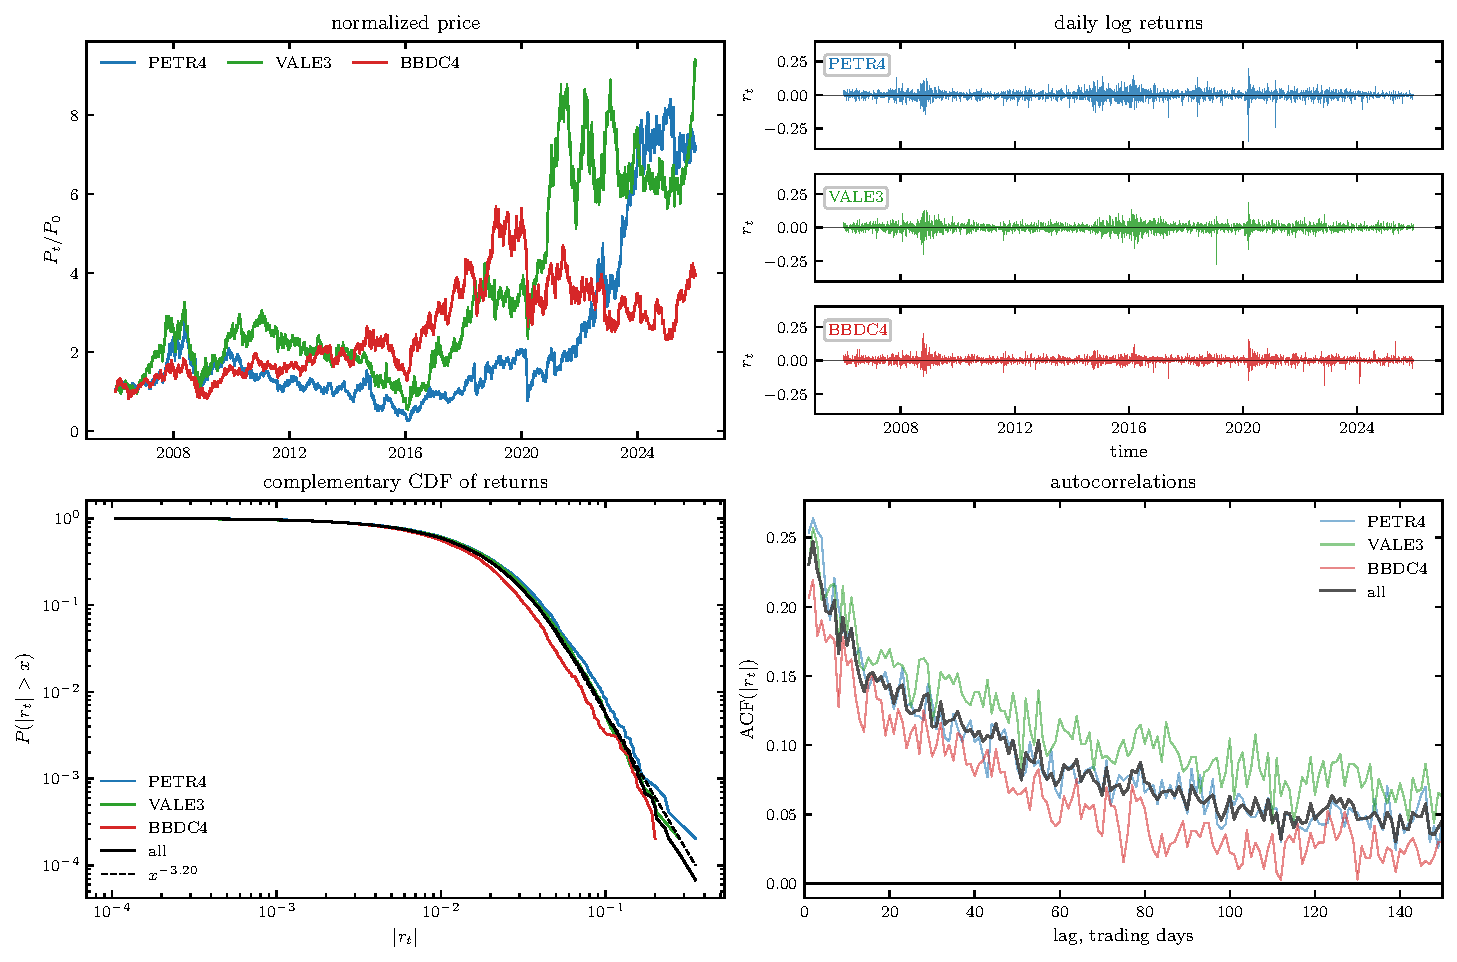
\includegraphics[width=0.95\linewidth]{images/figure_1d_stylized_facts_demo_assets_clean_2006_2025.pdf}
\captionof{figure}{Stylized facts for PETR4, VALE3 and BBDC4 over 2006--2025. The panels show normalized prices, daily log returns, the complementary cumulative distribution of absolute returns and autocorrelations of absolute returns. The return panel uses three vertically aligned subpanels with a common scale and a zero reference line for each asset.}
\label{fig:stylized_facts}
\end{center}

\normalsize

Taken together, the visual and numerical evidence shows that the selected B3 assets exhibit well-known empirical regularities of financial returns, including non-Gaussian behavior and volatility persistence. This motivates extending the analysis from individual return dynamics to the dependence structure across the broader equity universe.

We now turn from individual return behaviour to cross-sectional dependence. The core historical universe contains 58 assets, producing $N(N-1)/2=1653$ unique asset pairs. The static summaries use the available overlap for each pair and therefore retain the broader unbalanced historical coverage. The subsequent RMT analysis instead uses the complete synchronized 58-asset panel from 23 August 2006 to 15 August 2024. This distinction ensures that the descriptive correlation evidence is not confused with the common-sample correlation matrix used for the spectral decomposition. 

The pairwise correlations are positive on average but dispersed, and within-sector pairs tend to be more strongly related than pairs from different sectors. Figure~\ref{fig:correlation_structure} shows both the full distribution and the within-sector versus between-sector comparison. Across the broader unbalanced pair coverage, the mean is close to 0.24 and the median close to 0.23. This level of average dependence suggests the presence of a common component, but the distribution remains dispersed. The dispersion is important because it leaves room for sectoral and subsectoral organization instead of a single homogeneous market block.

The sectoral comparison provides a first indication that this heterogeneity is economically structured. Within-sector correlations are shifted toward higher values relative to between-sector correlations. As summarized in Table~\ref{tab:sector_corr_summary}, the mean within-sector correlation is 0.3433, compared with 0.2249 for between-sector pairs, producing a difference of $\Delta_{\mathrm{sector}}=0.1184$.

\begin{center}
\begin{minipage}{0.5\linewidth}
  \centering
  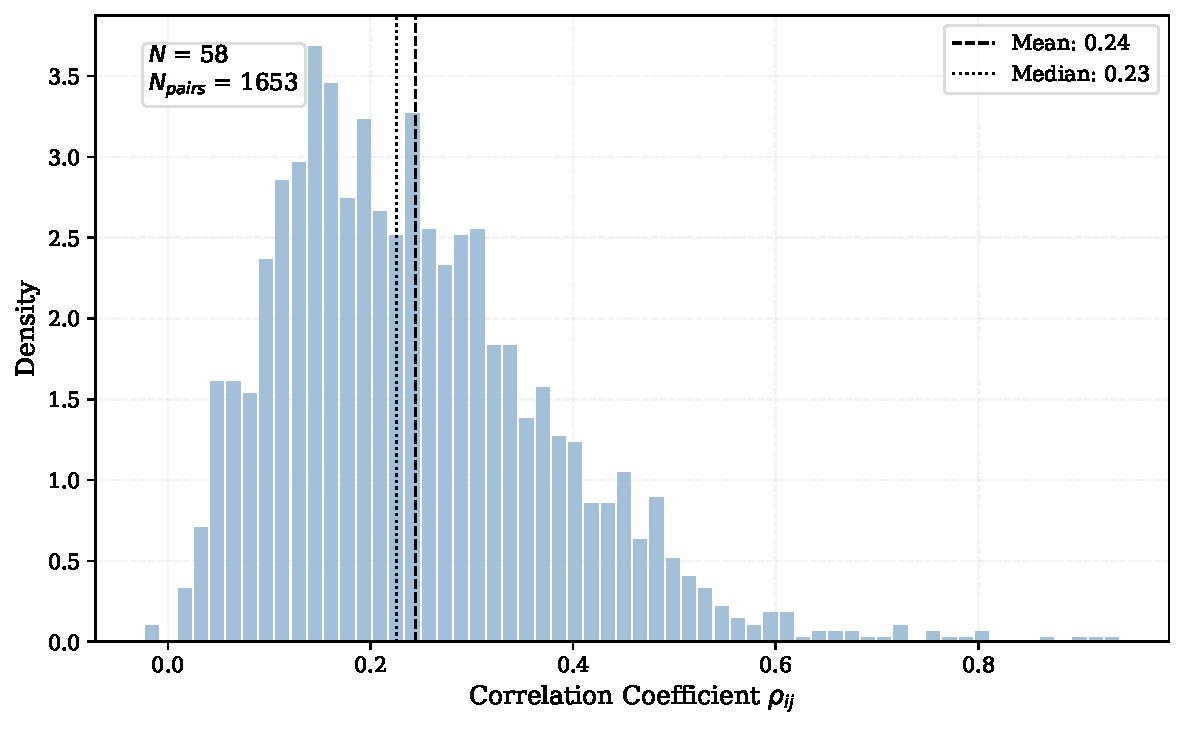
\includegraphics[width=\linewidth]{images/figure_2_correlation_histogram.pdf}
  \vspace{0.2cm}

  \small (a) Full pairwise distribution.
\end{minipage}
\hfill
\begin{minipage}{0.48\linewidth}
  \centering
  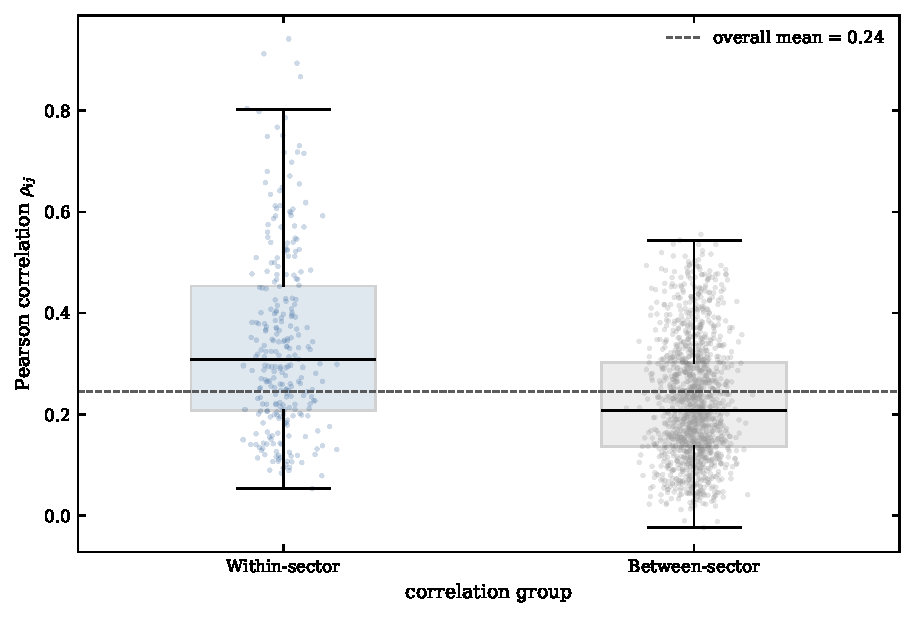
\includegraphics[width=\linewidth]{images/figure_3_sector_correlation_distribution.pdf}
  \vspace{0.2cm}

  \small (b) Within-sector and between-sector pairs.
\end{minipage}

\captionof{figure}{Correlation structure in the core historical universe. Panel (a) shows the full Pearson correlation distribution. Panel (b) compares within-sector and between-sector correlations using the initial macro-sector classification.}
\label{fig:correlation_structure}
\end{center}

\begin{center}
\captionof{table}{Within-sector and between-sector correlation summary.}
\label{tab:sector_corr_summary}
\begin{tabular}{lrrrrrr}
\toprule
Group & Pairs & Mean & Median & Std. dev. & Min & Max \\
\midrule
Within-sector & 275 & 0.3433 & 0.3082 & 0.1819 & 0.0534 & 0.9402 \\
Between-sector & 1378 & 0.2249 & 0.2076 & 0.1166 & -0.0236 & 0.5552 \\
\bottomrule
\end{tabular}
\end{center}


The difference is economically meaningful. Within-sector pairs have mean correlation 0.3433, while between-sector pairs have mean correlation 0.2249, giving $\Delta_{\mathrm{sector}}=0.1184$. An asset-level label-permutation test with 10,000 sector-label reallocations preserves both the observed dependency matrix and the sector-size vector, without treating overlapping pairs as independent observations. None of the permuted statistics reaches the observed difference (null 95th percentile $=0.0245$; one-sided Monte Carlo $p\approx 10^{-4}$, the minimum attainable at this simulation count). The observed difference is also supported by the sector-label permutation analysis reported later in the robustness assessment. At this stage, the relevant result is that the dependency matrix is not characterized solely by homogeneous positive co-movement: stronger relationships are also concentrated within the economic grouping used in the analysis.

The static correlation distribution, however, does not show whether these relationships remain stable through time. We therefore examine selected economically interpretable asset pairs under different dynamic correlation estimators. Figure~\ref{fig:dynamic_pairwise} includes PETR4--VALE3, representing two large commodity-exposed firms in distinct subsectors; BBDC4--BBAS3 in financials; GGBR4--USIM5 in steel and metallurgy; and ELET3--CMIG4 in utilities. These pairs are illustrative rather than intended to represent all possible pairwise relationships.

The pairwise estimates show that individual dependencies can strengthen, weaken, or temporarily break down over time. The 20-day Pearson estimates respond rapidly to local variation, whereas the 60-day estimates provide smoother representations of persistent relationships. The EWMA estimates provide an intermediate view by assigning greater weight to recent observations. The common conclusion across these estimators is that a single full-sample correlation should be interpreted as a long-run summary of an underlying time-varying relationship.

We finally move from individual pairs to market-wide synchronization. Figure~\ref{fig:rolling_corr} reports the average pairwise market correlation estimated with 252- and 504-trading-day rolling windows. Because historical coverage changes in the earliest part of the sample, each window uses the assets available during that period, ranging from approximately 40 assets initially to the complete 58-asset universe in later years. The series should therefore be interpreted as a descriptive measure of average available cross-sectional dependence.

Market-wide correlation varies through time and increases around the 2008 global financial crisis and the 2020 COVID-19 shock. Figure~\ref{fig:rolling_corr} remains close to 0.2 during 2015--2016, so that interval does not show a comparable increase in this measure. These episodes show that the positive dependence observed in the static correlation distribution is not constant through time.

Taken together, the results reveal three complementary features of the B3 dependency structure: positive but heterogeneous cross-sectional correlations, stronger dependence within economic sectors, and substantial variation in synchronization over time. The presence of broad co-movement alongside more localized relationships raises the next question in the empirical sequence: how much of the observed correlation structure is associated with a dominant collective market mode, how much remains in smaller group-level components, and how much is compatible with sampling noise? We address this question next through Random Matrix Theory.

\begin{center}
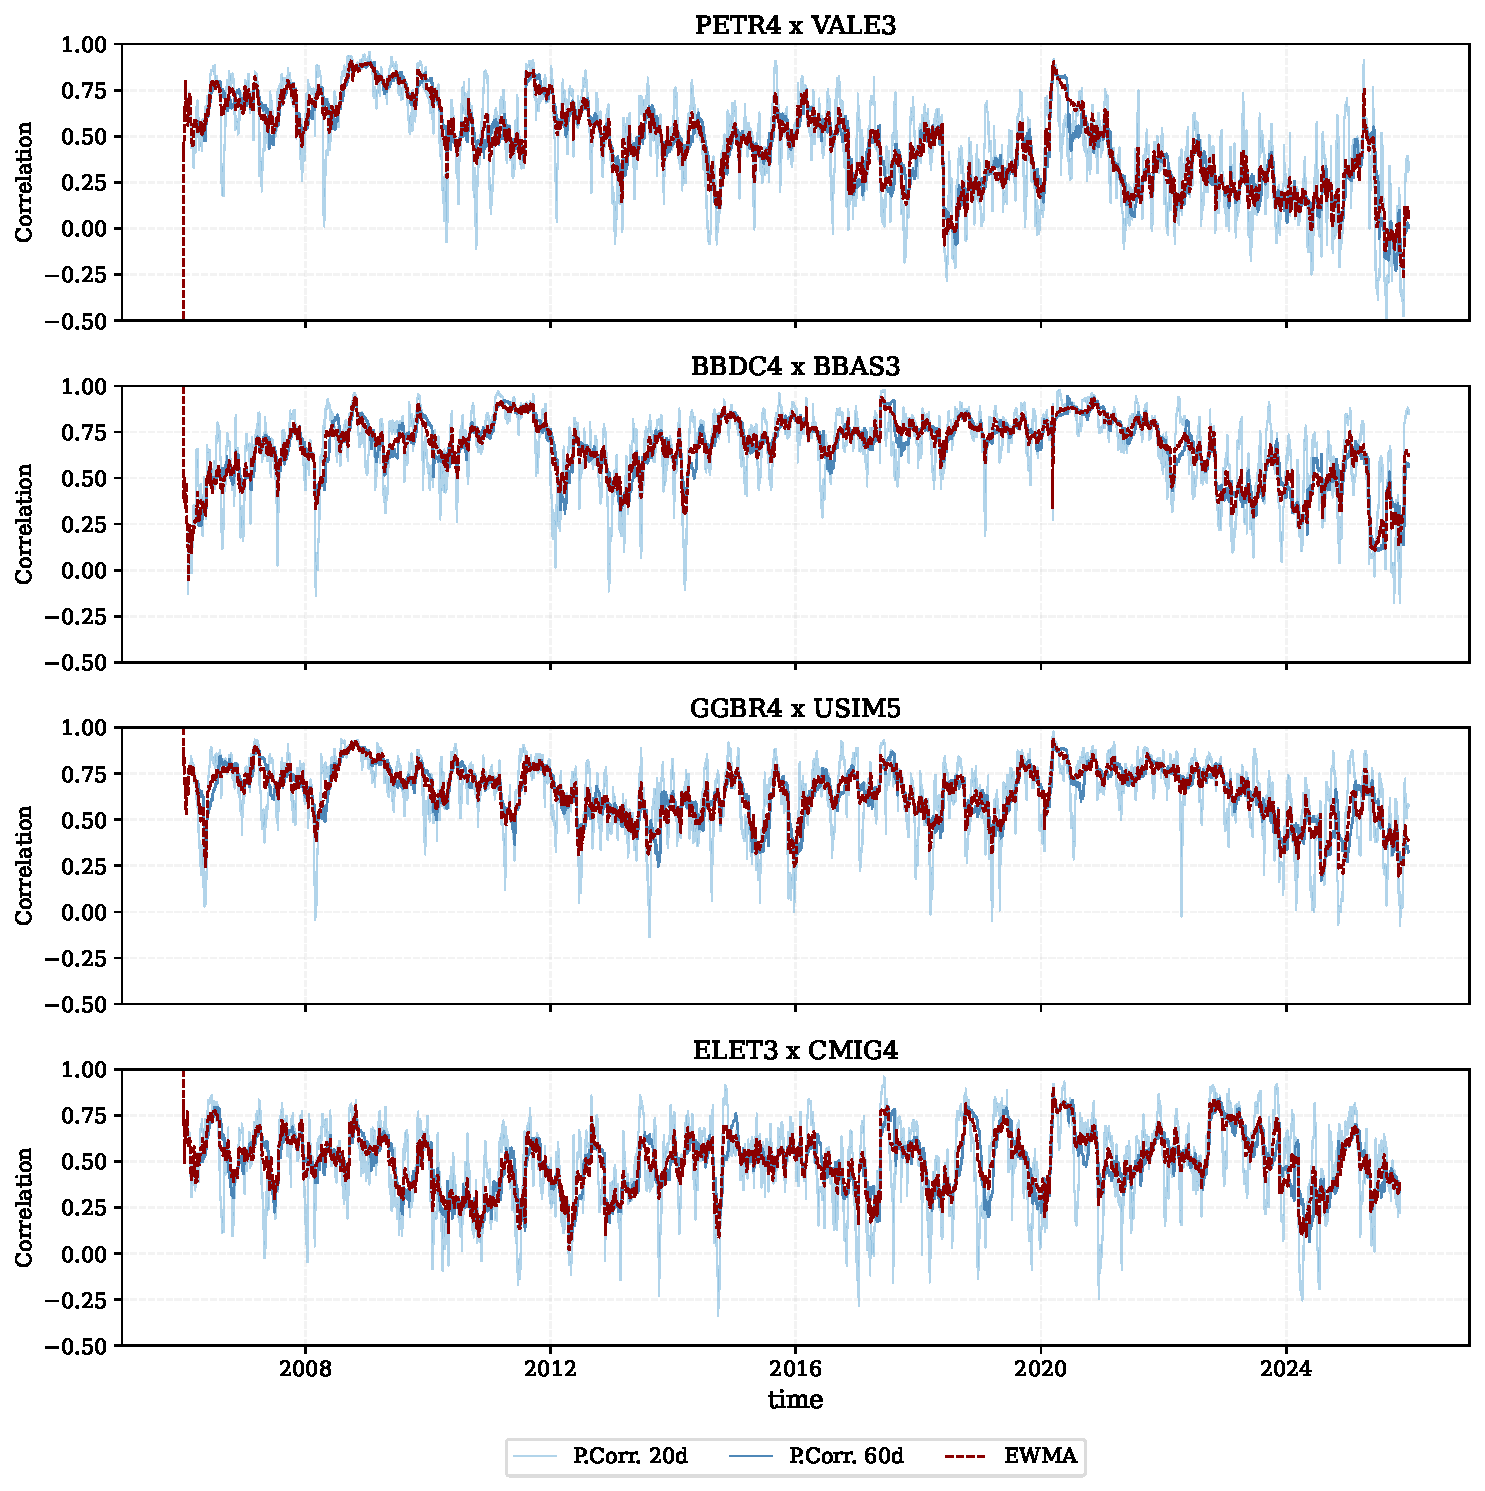
\includegraphics[width=\linewidth]{images/figure_5_dynamic_pairwise_correlations.pdf}
\captionof{figure}{Dynamic pairwise correlations for selected economically interpretable asset pairs. Pearson estimates use 20- and 60-trading-day windows; EWMA uses a 20-day half-life. The estimates show how individual dependencies can vary across time scales.}
\label{fig:dynamic_pairwise}
\end{center}


\begin{center}
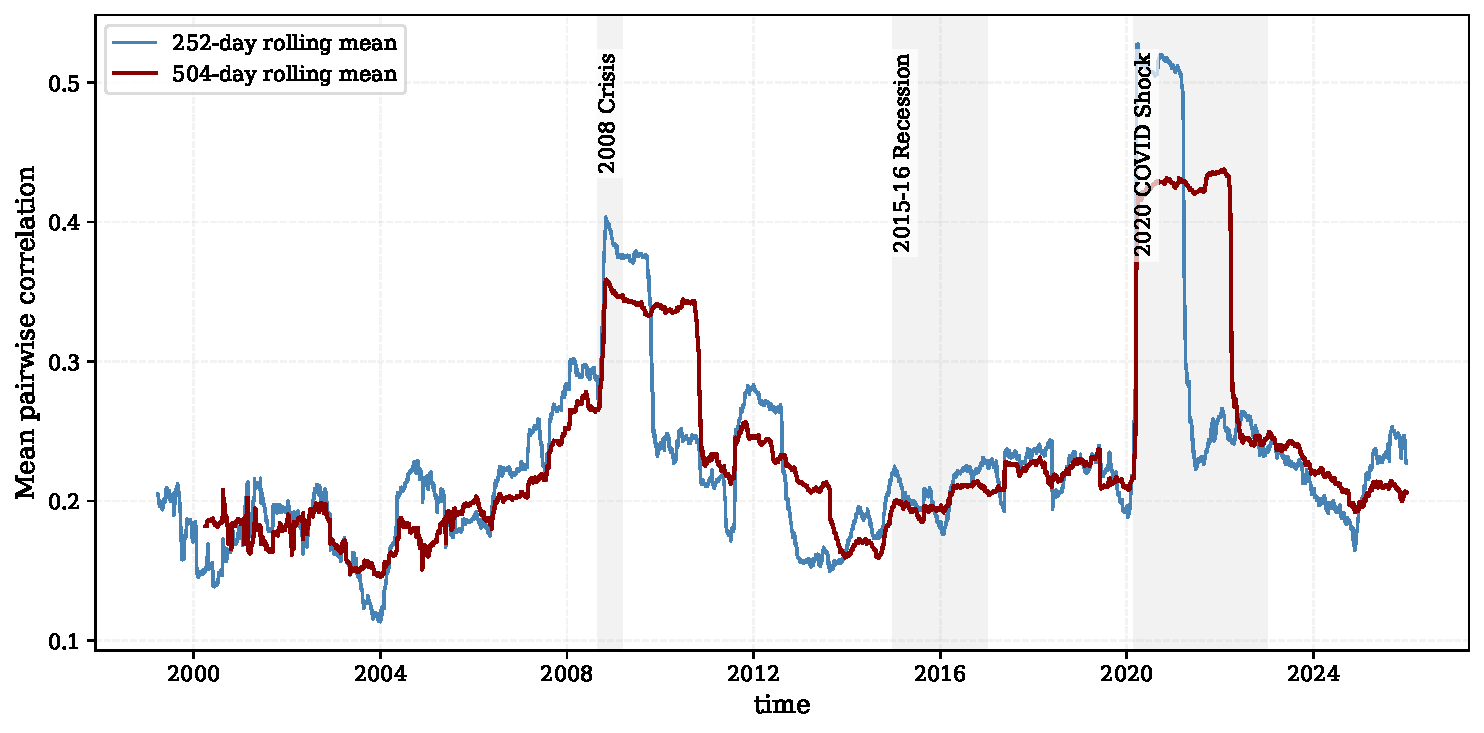
\includegraphics[width=0.95\linewidth]{images/figure_4_rolling_average_correlation.pdf}
\captionof{figure}{Rolling average market correlation for the core historical universe, estimated with 252- and 504-trading-day windows. Each window uses the assets available during that period.}
\label{fig:rolling_corr}
\end{center}


\subsection{Spectral Structure Beyond the Market Mode}
\label{sec:rmt}

The dependence patterns identified in Section~\ref{sec:stylized_correlation} raise a central question: how much of the observed correlation structure reflects broad market synchronization, and how much remains in smaller collective components beyond the sampling-noise benchmark. Following the RMT procedure described in Section~\ref{subsec:rmt_method}, we examine the eigenspectrum of the complete synchronized panel of $N=58$ assets and $T=1527$ observations.

\subsubsection{Empirical Eigenspectrum and Mode Separation
}


For this panel, $Q=T/N=26.33$, yielding Mar\v{c}enko--Pastur bounds of $\lambda_-=0.6482$ and $\lambda_+=1.4278$. Five empirical eigenvalues lie above the upper bound, comprising the market eigenvalue and four additional non-market modes. The mean off-diagonal correlation on this same synchronized $58\times1527$ panel is 0.3350, whereas the leading eigenvalue accounts for 0.3733 of the trace. These are related but distinct summaries: the pairwise mean averages 1,653 correlations, while $\lambda_1/N$ is the leading spectral share and need not equal the mean correlation in a heterogeneous matrix. The approximately 0.24 mean shown for the broader pairwise summaries uses unbalanced pair coverage and a different sample definition.

Table~\ref{tab:rmt_summary} reports the numerical inputs for RMT filtering. The leading eigenvalue, $\lambda_1=21.6505$, is substantially larger than the remaining eigenvalues and accounts for approximately 37.3\% of the total trace of the correlation matrix. The next four eigenvalues, $\lambda_2=3.0957$, $\lambda_3=1.7839$, $\lambda_4=1.6543$, and $\lambda_5=1.4835$, also exceed $\lambda_+$, indicating additional candidate collective structures beyond the dominant market component.

\begin{center}
\captionof{table}{Summary of the RMT eigenspectrum for the complete 58-asset panel.}
\label{tab:rmt_summary}
\setlength{\tabcolsep}{4pt}
\begin{tabular}{rrrrrrr}
\toprule
$N$ & $T$ & $Q$ & $\lambda_-$ & $\lambda_+$ &
Eigenvalues above $\lambda_+$ (total; non-market) & Market-mode share \\
\midrule
58 & 1527 & 26.33 & 0.6482 & 1.4278 & 5 (4) & 37.33\% \\
\bottomrule
\end{tabular}
\end{center}


Figure~\ref{fig:rmt_spectrum} places these eigenvalues against the Mar\v{c}enko--Pastur benchmark. The separation of $\lambda_1$ from both the noise-compatible region and the remaining significant modes provides the first evidence of a dominant collective market component. At the same time, the presence of four additional eigenvalues above $\lambda_+$ indicates that the correlation structure cannot be reduced to market-wide synchronization alone.

The leading eigenvector has positive loadings across the asset universe and therefore represents broad market co-movement. Because this component accounts for approximately 37.3\% of the total trace, it can dominate the structure of the original correlation matrix and obscure weaker localized relationships. We therefore remove the leading mode and reconstruct the component associated with the remaining eigenvalues above the Mar\v{c}enko--Pastur upper bound.

Spectral reconstruction reproduces the original correlation matrix up to floating-point precision, confirming that the subsequent differences between the original and filtered representations arise from the intended mode separation rather than numerical reconstruction error. The complete component-by-component matrix display is provided in supplementary Figure~\ref{fig:rmt_full_components_supplement}; it shows the retained and noise-compatible components that are summarized here.

\begin{center}
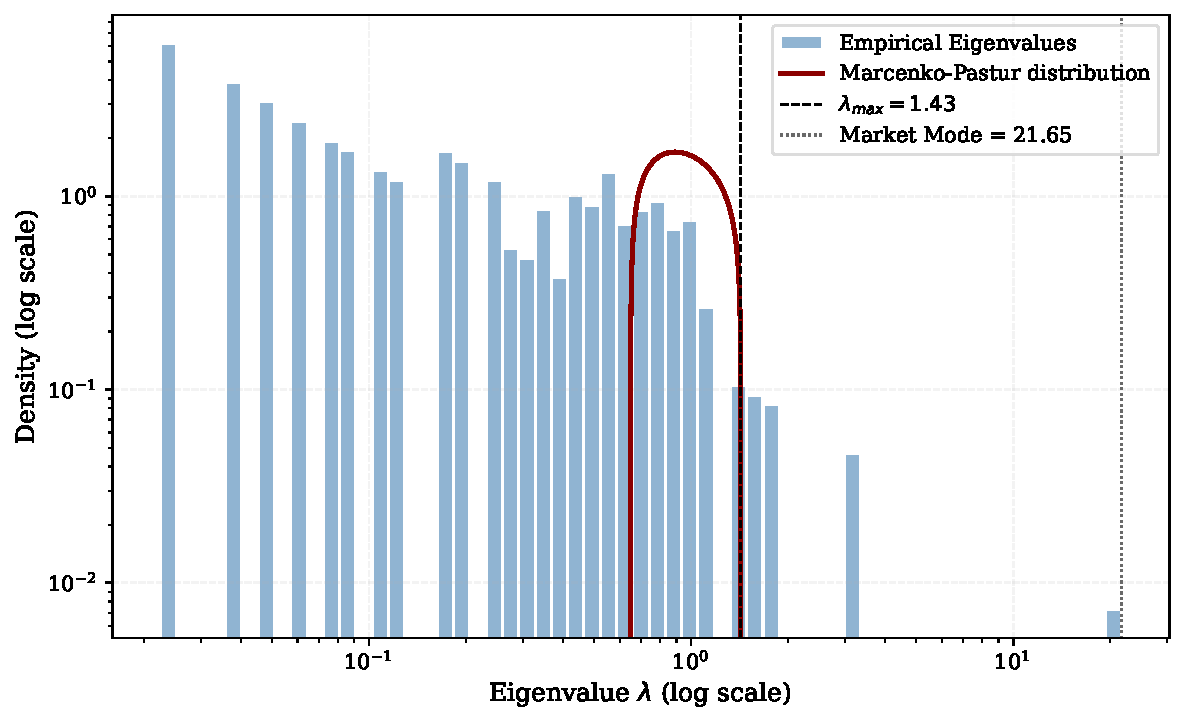
\includegraphics[width=0.85\linewidth]{images/figure_6_rmt_eigenvalue_spectrum.pdf}
\captionof{figure}{Empirical eigenvalue spectrum and Mar\v{c}enko--Pastur bounds. The largest eigenvalue is far outside the random band and captures the market-mode component.}
\label{fig:rmt_spectrum}
\end{center}

Figure~\ref{fig:rmt_filtered_matrices} shows the effect of this separation. The original matrix is dominated by broadly positive correlations, consistent with the strong collective component identified in the eigenspectrum. After removal of the leading mode, the candidate group-mode component reveals a more heterogeneous pattern, with localized positive and negative contrasts that were less visible in the original matrix.
\begin{center}
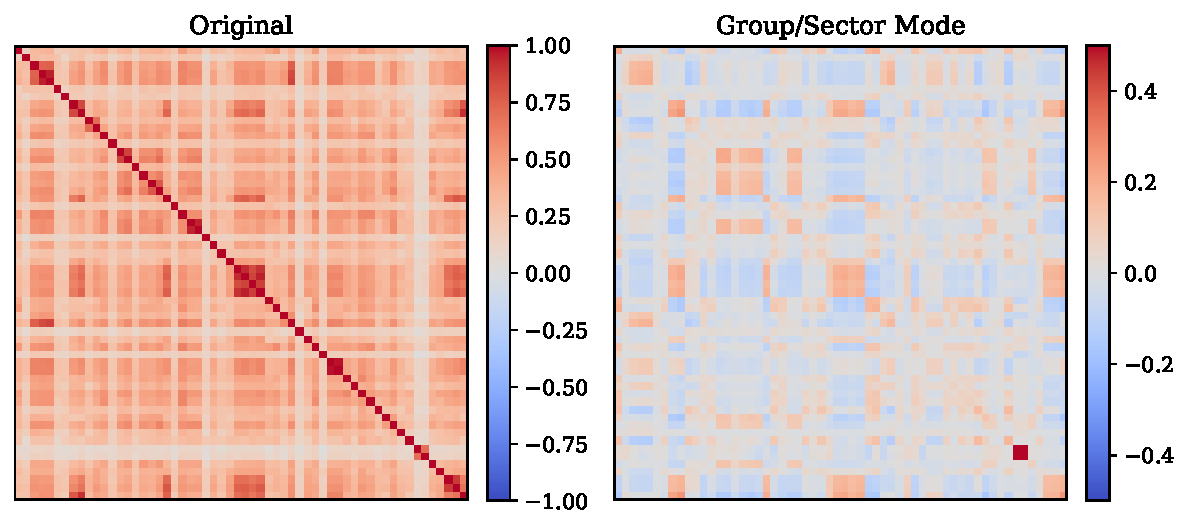
\includegraphics[width=0.9\linewidth]{images/figure_8_original_group_matrices.pdf}
\captionof{figure}{Original and candidate group-mode RMT component matrices at readable scale. The original matrix is dominated by broad positive co-movement, whereas the group-mode component highlights weaker localized contrasts after the leading market mode is removed.}
\label{fig:rmt_filtered_matrices}
\end{center}

The persistence of structured contrasts after market-mode removal suggests that the significant non-leading modes are not merely weaker copies of the collective component. Their composition must therefore be examined directly through their eigenvector loadings before determining whether the same organization reappears in hierarchical and network representations.

\subsubsection{Composition of the Significant Spectral Modes}

Eigenvalues indicate the strength of collective modes, while their eigenvectors reveal how individual assets contribute to each component. Figure~\ref{fig:eigenvector_loadings} reports the largest loadings for the five eigenvalues above the Mar\v{c}enko--Pastur upper bound. Assets are ranked by loading magnitude within each eigenvector. Because the overall sign of an eigenvector is arbitrary, the interpretation focuses on the relative contrasts, magnitude, and concentration of the loadings.

\begin{center}
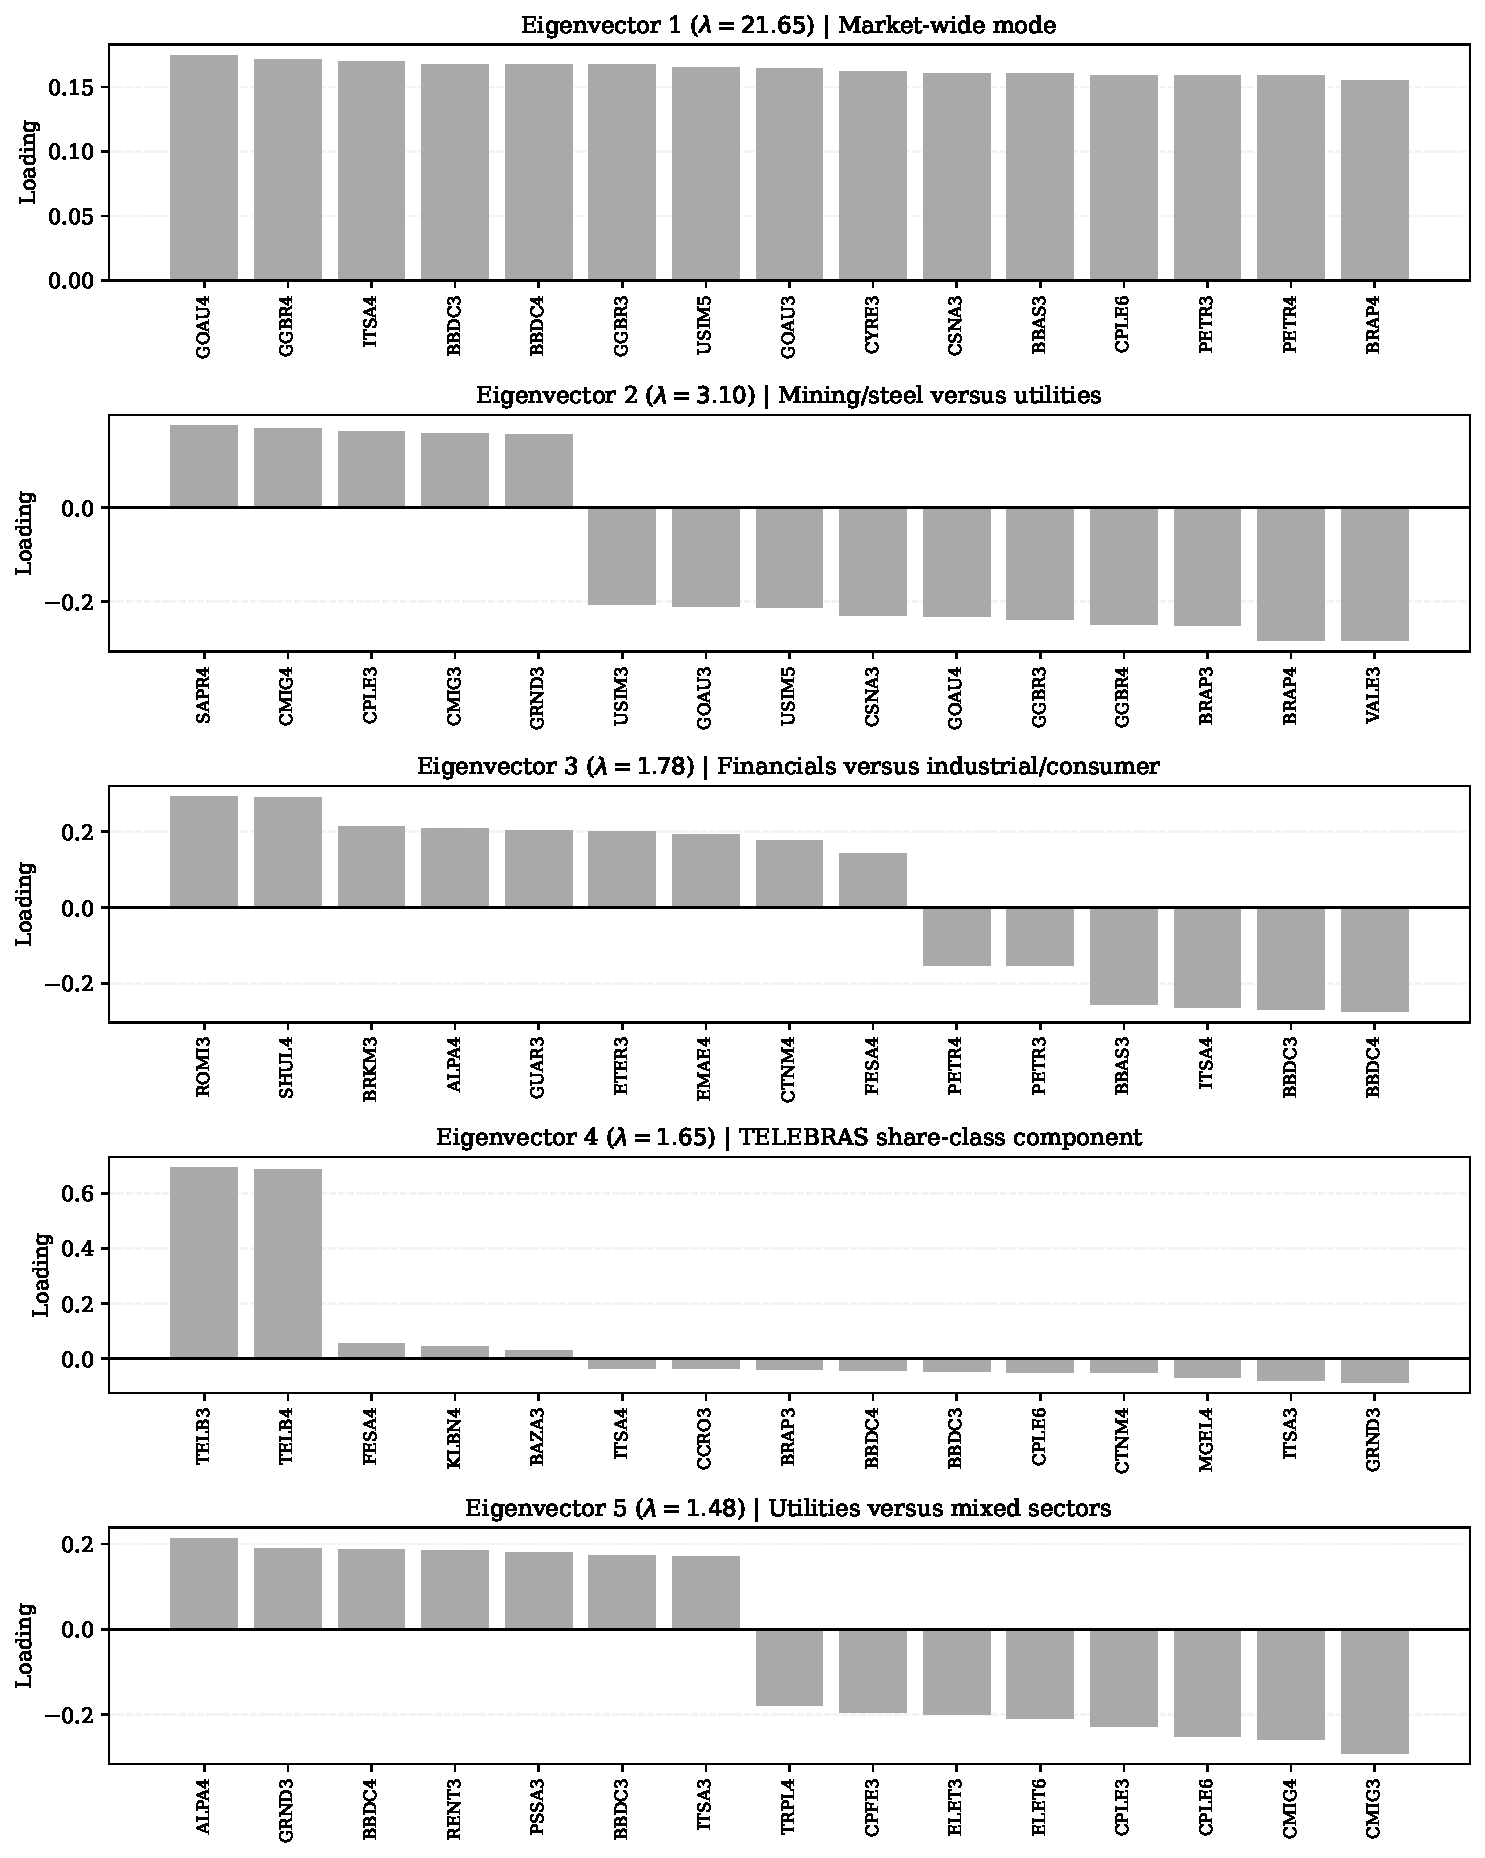
\includegraphics[width=0.95\linewidth]{images/figure_7b_rmt_top_eigenvectors_top_loadings.pdf}
\captionof{figure}{Top eigenvector loadings for the five RMT modes above the Mar\v{c}enko--Pastur upper bound. Eigenvector 1 is a broad market mode. Subsequent eigenvectors show relative contrasts between groups of assets; their overall signs are arbitrary.}
\label{fig:eigenvector_loadings}
\end{center}

The first eigenvector exhibits positive loadings across all 58 assets, ranging from 0.037 to 0.174. Its contribution is distributed across multiple sectors rather than concentrated in a single economic group, reinforcing the interpretation of the leading component as a broad market mode.

The second eigenvector ($\lambda_2=3.10$) is best read as a relative contrast between mining and steel firms---including VALE3, BRAP3/4, GGBR3/4, GOAU3/4, CSNA3 and USIM3/5---and a group led by utilities and selected consumer-cyclical assets. It therefore contains a commodity-related dimension, but it is not a pure Basic Materials factor.

The third eigenvector ($\lambda_3=1.78$) similarly contrasts the financial pole formed by BBDC3/4, ITSA4 and BBAS3 with a more heterogeneous industrial, chemical and consumer-cyclical pole led by ROMI3, SHUL4, BRKM3, ALPA4 and GUAR3.

The fourth eigenvector ($\lambda_4=1.65$) is highly concentrated in TELB3 and TELB4, the two listed TELEBRAS share classes. We interpret this result as an issuer-specific share-class component, rather than as evidence of a broad telecommunications factor. 

The fifth eigenvector ($\lambda_5=1.48$) separates a coherent utilities block---including CEMIG, COPEL, Eletrobras, CPFL Energia and ISA CTEEP---from financial and selected consumer-cyclical assets. This is a plausible utilities-related pattern, but $\lambda_5$ lies only about 3.7\% above the Mar\v{c}enko--Pastur upper bound. Its economic interpretation should therefore remain cautious and be treated as a candidate localized mode.

Overall, Figure~\ref{fig:eigenvector_loadings} shows that the modes beyond the dominant market component are structured contrasts rather than simple one-sector classifications. Some modes align partially with recognizable economic groups, while others reflect more localized or issuer-specific relationships. This motivates the subsequent hierarchical and network analyses, which examine whether these spectral patterns reappear in alternative representations of the dependency structure.


\subsection{Hierarchical and Network Organization After Spectral Filtering}
\label{sec:network_organization}

The spectral analysis in Section~\ref{sec:rmt} showed that removing the dominant market mode reveals weaker but structured dependencies among groups of assets. We now examine whether these patterns also appear in the distance geometry of the correlation matrices. Hierarchical ordering provides a complementary representation of the same dependency structure, allowing localized organization to be compared across the original and RMT-filtered matrices.

\subsubsection{Hierarchical Organization of the Filtered Dependence Structure}
\label{sec:clustering}

Figure~\ref{fig:ordered_heatmaps} shows the correlation matrices after hierarchical ordering. The original matrix retains a broad positive background, consistent with the dominant collective component identified in the eigenspectrum. After spectral filtering, this common background is reduced and localized blocks become more visible. The group-mode representation is particularly informative because it emphasizes relative dependencies that remain after removal of the leading market component.

\begin{center}
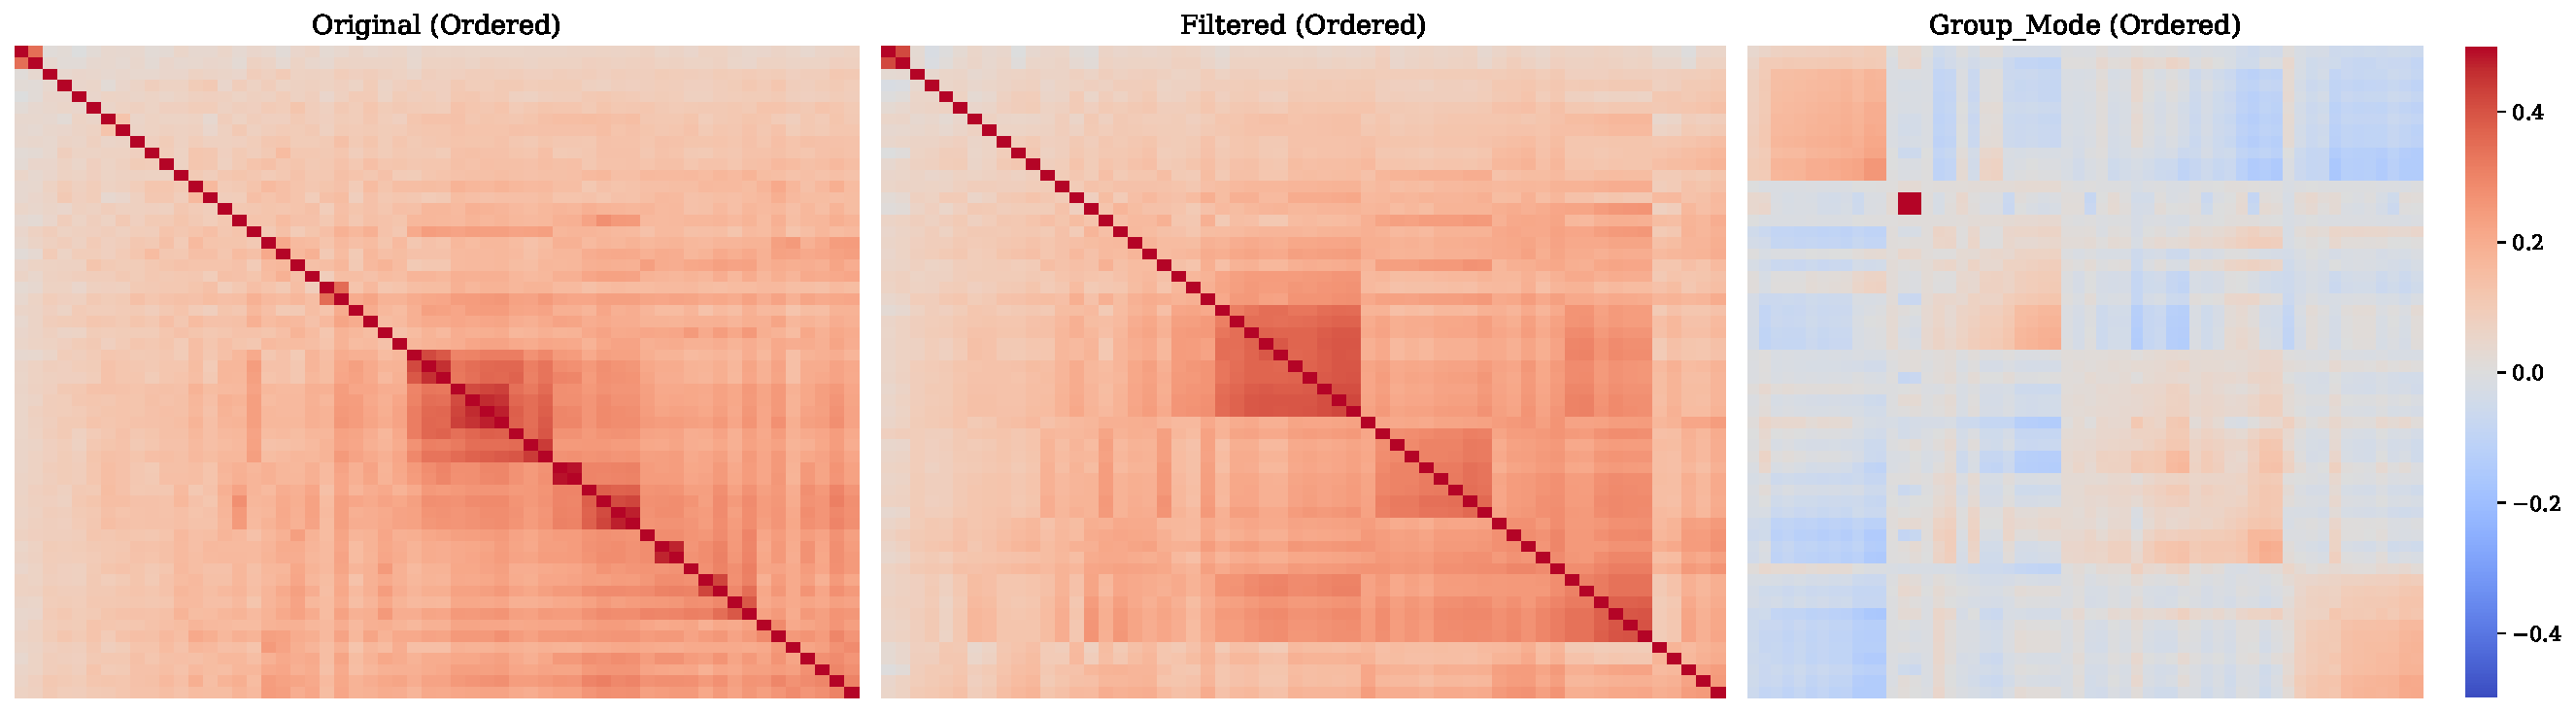
\includegraphics[
width=\linewidth,
height=0.72\textheight,
keepaspectratio
]{images/figure_10_ordered_heatmaps.pdf}
\captionof{figure}{Hierarchically ordered correlation matrices for the original and RMT-filtered structures. The common color scale highlights the reduction of broad market-wide co-movement and the emergence of more localized dependency patterns after spectral filtering.}
\label{fig:ordered_heatmaps}
\end{center}

The ordered matrices indicate that market-mode removal does not eliminate organization from the dependency structure. Instead, it changes its scale: the broad positive background becomes weaker while smaller blocks of relatively stronger and weaker relationships become easier to distinguish. These patterns are consistent with the heterogeneous compositions observed in the non-leading eigenvectors and suggest that part of the residual spectral structure is also expressed geometrically.

The corresponding hierarchical tree provides a more compact view of this organization. Figure~\ref{fig:dendrograms} shows the group-mode dendrogram obtained from Mantegna distances and average linkage. To shorten the long horizontal branches, the plotted merge heights use a monotone logarithmic transform; the tick labels report the original distances. Macro-sector colors are included only as an external reference for interpretation; the clustering procedure itself does not impose sector labels.

\begin{center}
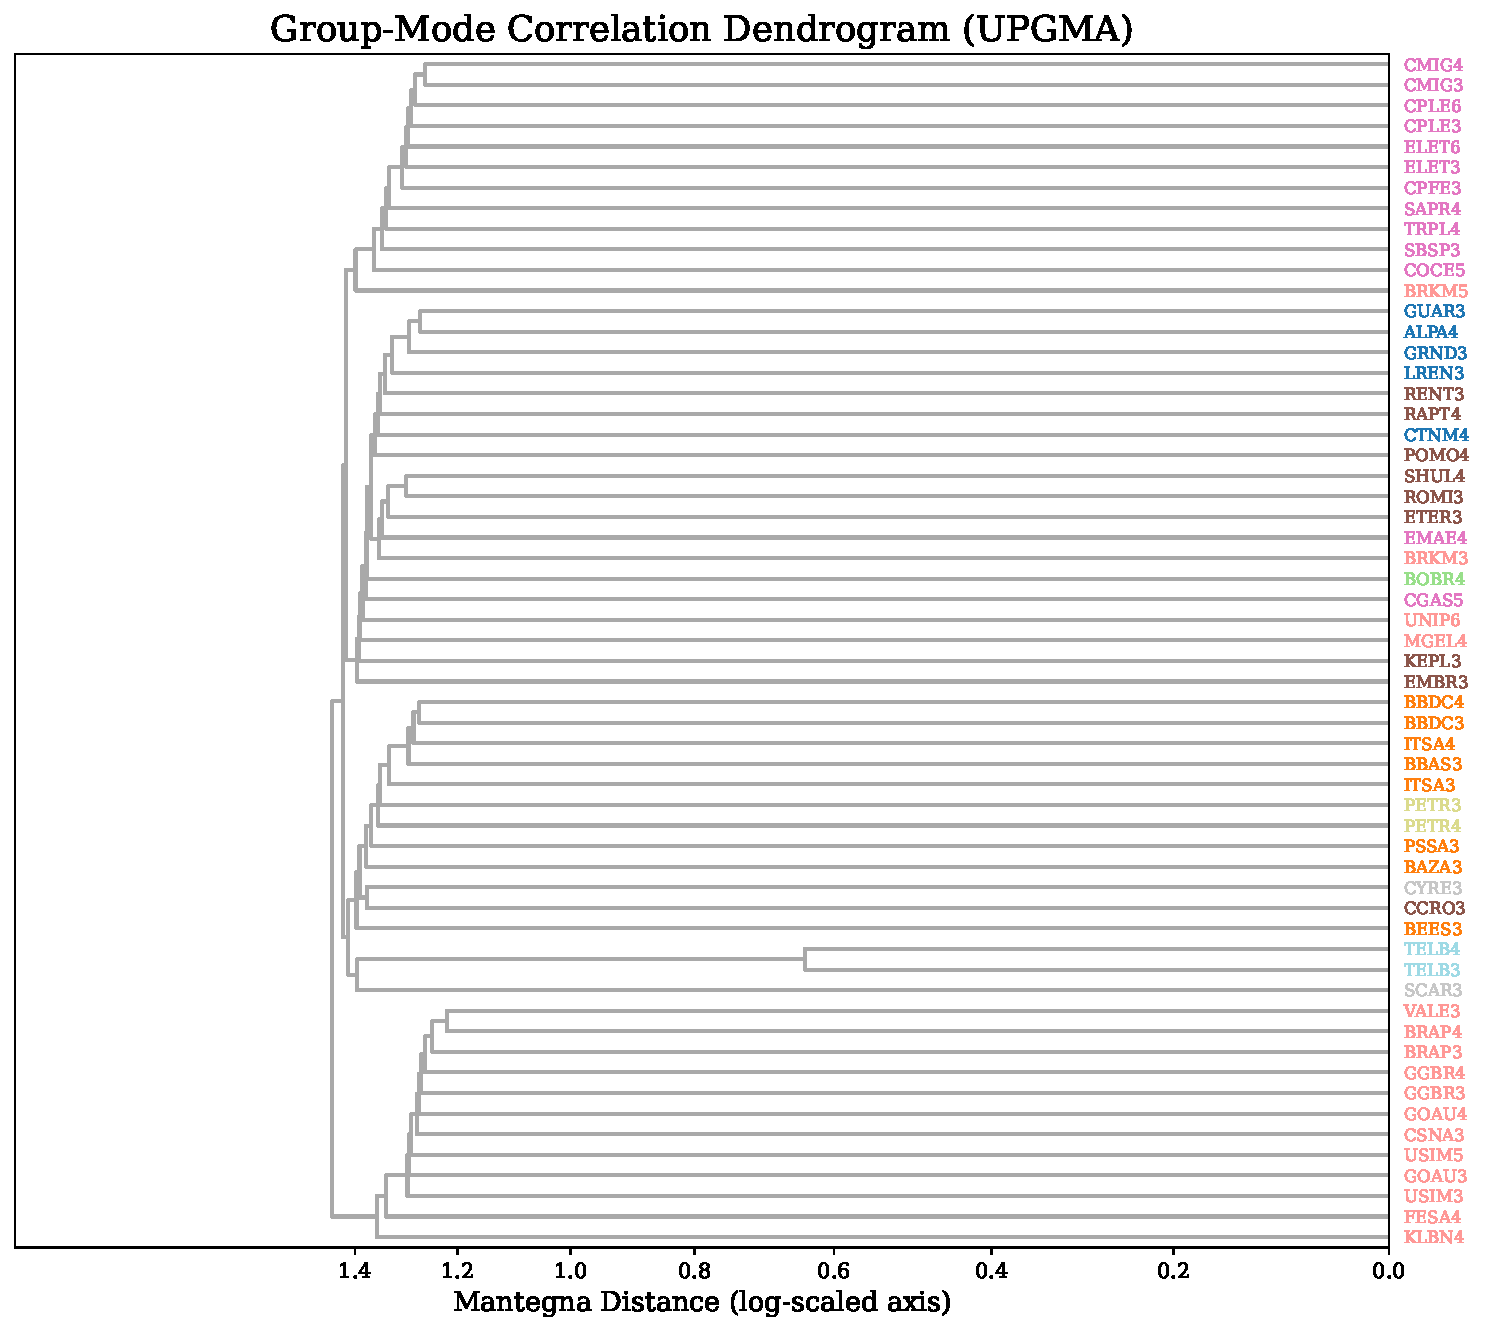
\includegraphics[
width=0.82\linewidth,
height=0.8\textheight,
keepaspectratio
]{images/figure_9_group_mode_dendrogram.pdf}
\captionof{figure}{Group-mode dendrogram obtained from Mantegna distances and average linkage. The horizontal axis uses a monotone log transformation, with tick labels in the original distance scale. The tree summarizes the dependency geometry remaining after removal of the dominant market mode; label colors indicate the initial macro-sector classification for comparison.}
\label{fig:dendrograms}
\end{center}

Table~\ref{tab:cophenetic_summary} compares how closely the hierarchical trees preserve the underlying distance structures.

\begin{center}
\captionof{table}{Cophenetic correlations for the original and RMT-filtered dependency structures.}
\label{tab:cophenetic_summary}
\begin{tabular}{lrr}
\toprule
Matrix & Assets & Cophenetic correlation \\
\midrule
Original & 58 & 0.950 \\
Filtered & 58 & 0.934 \\
Group-mode & 58 & 0.871 \\
\bottomrule
\end{tabular}
\end{center}


The supplementary Figure~\ref{fig:dendrograms_full_supplement} compares the original, filtered and group-mode trees side by side; it shows the additional geometric context for the focused group-mode tree in Figure~\ref{fig:dendrograms}. The original matrix has the highest cophenetic correlation, at 0.950, followed by the filtered matrix at 0.934 and the group-mode matrix at 0.871. The decline after market-mode removal indicates that the residual dependency structure is less accurately represented by a strictly hierarchical tree. This does not imply the disappearance of localized organization; rather, it suggests that the remaining geometry is more complex than the broad market-dominated structure observed in the original matrix.

The hierarchical analysis therefore provides two complementary findings. First, localized dependency patterns remain visible after removal of the dominant market component. Second, these relationships become less purely tree-like as the common market structure is removed. This motivates moving from hierarchical representations to graph-based filtering, where additional connections can be retained and the reorganization of hubs, local connectivity, and sectoral relationships can be examined directly.


\subsubsection{Network Topology Before and After Market-Mode Removal}
\label{sec:networks}

The hierarchical analysis showed that localized dependency patterns remain after removal of the dominant market component, although the resulting geometry becomes less purely tree-like. We therefore move to graph-based representations, which retain selected dependency links and allow changes in connectivity, local organization, and centrality to be examined directly. We compare networks constructed from the original correlation matrix with those obtained from the group-mode component identified through RMT.

The Minimum Spanning Tree (MST) provides the sparsest connected representation of the dependency structure. With $N=58$ assets, each MST contains 57 edges. Figure~\ref{fig:mst_refined} compares the original and group-mode backbones.

\begin{center}
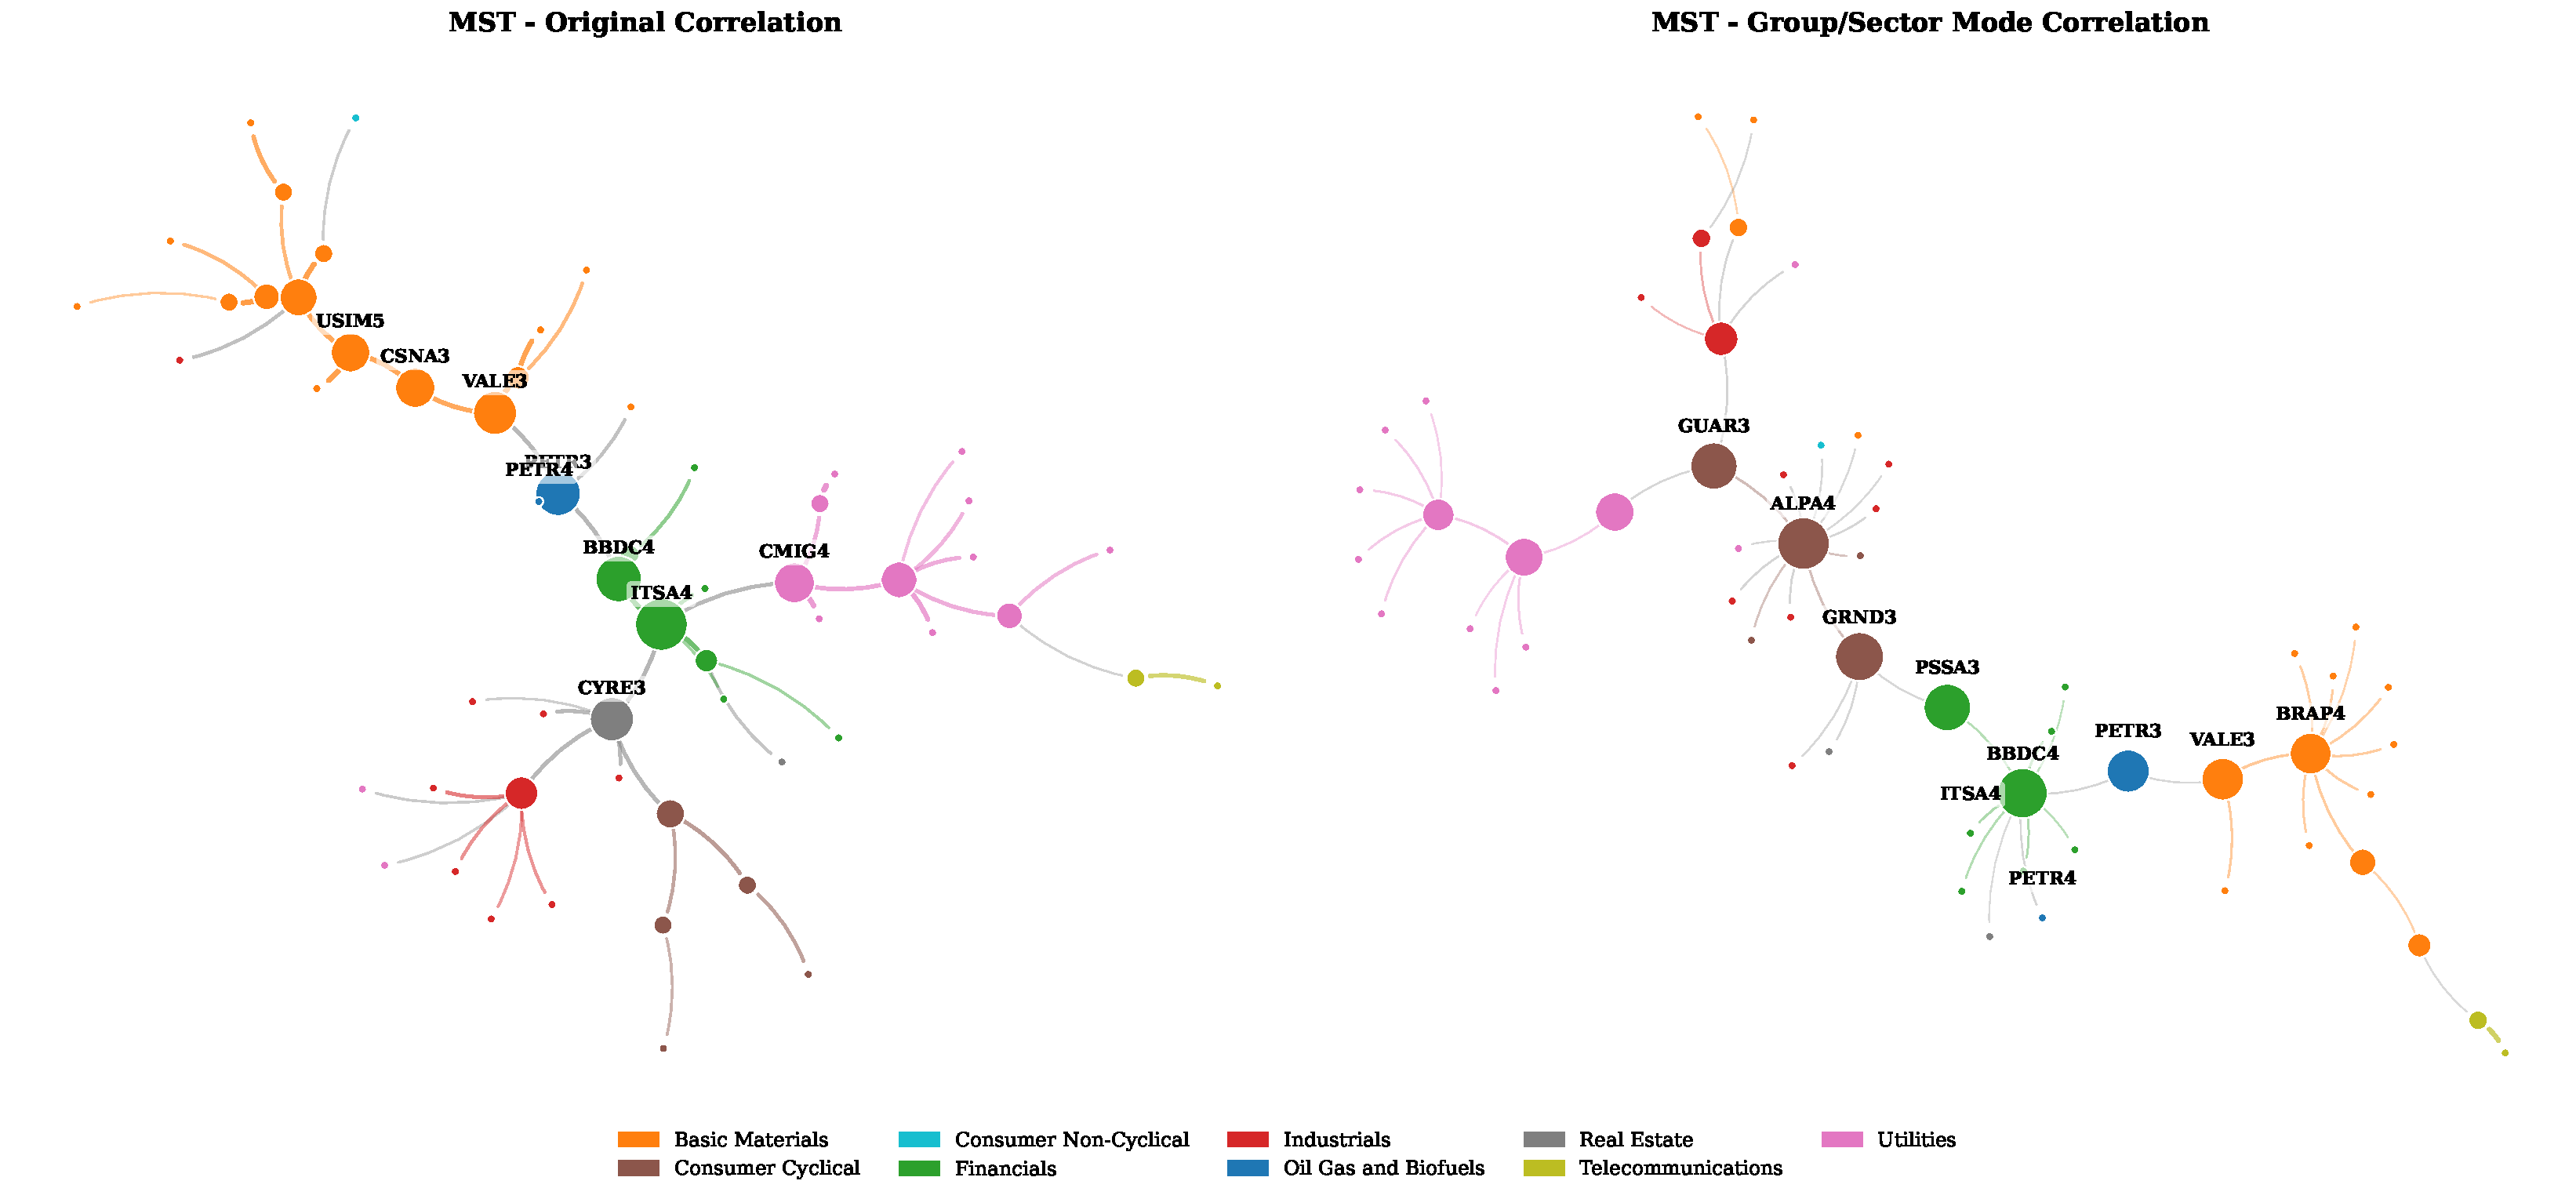
\includegraphics[
width=\linewidth,
height=0.58\textheight,
keepaspectratio
]{images/figure_11b_mst_refined_comparison.pdf}
\captionof{figure}{MST comparison for the original and group-mode correlation structures. Removal of the dominant market component changes the set of strongest dependency channels retained in the network backbone.}
\label{fig:mst_refined}
\end{center}

The original MST has a mean edge correlation of 0.5796, compared with 0.1388 for the group-mode MST. This reduction is expected because the latter excludes the dominant common component. More importantly, the same-sector edge ratio decreases from 0.7193 to 0.6316, indicating that the topology is reorganized rather than simply weakened. The group-mode MST therefore represents a different dependency backbone, emphasizing relationships that remain after broad market synchronization is removed.

The Planar Maximally Filtered Graph (PMFG) provides a richer representation of the same dependency geometry. Unlike the MST, the PMFG retains $3N-6=168$ edges and allows cycles, triangles, and cliques to remain in the graph. Figure~\ref{fig:pmfg_refined} compares the original and group-mode PMFGs.

\begin{center}
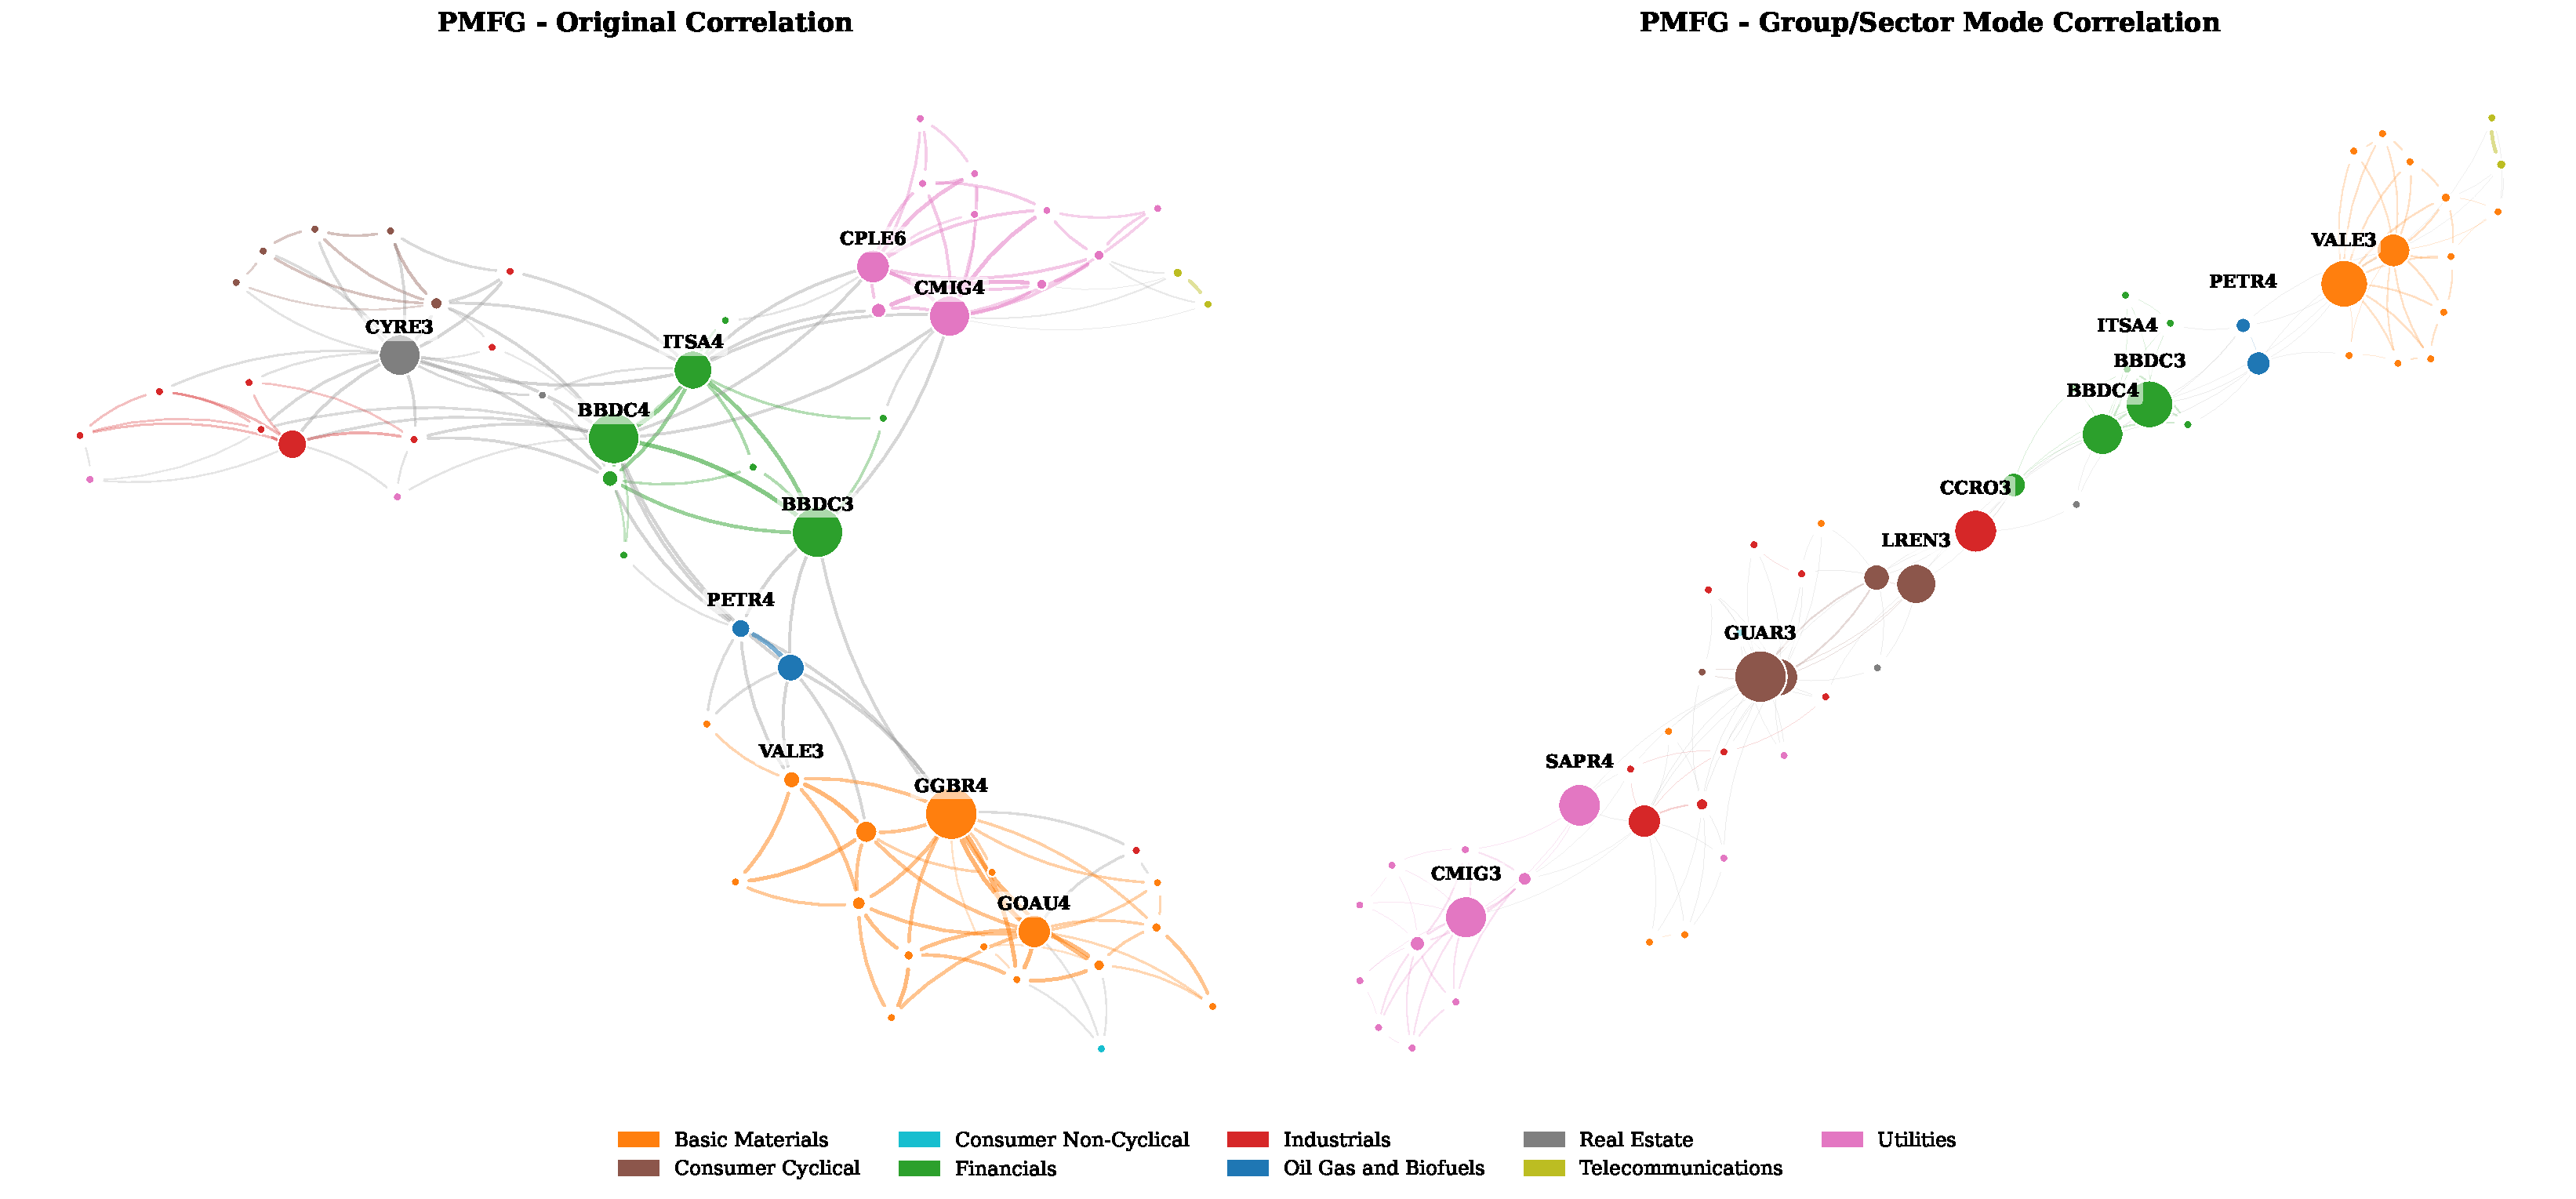
\includegraphics[
width=\linewidth,
height=0.58\textheight,
keepaspectratio
]{images/figure_12b_pmfg_refined_comparison.pdf}
\captionof{figure}{PMFG comparison for the original and group-mode correlation structures. The group-mode representation removes broad market-wide dominance while retaining a denser set of localized dependency relationships.}
\label{fig:pmfg_refined}
\end{center}

As in the MST, average edge strength decreases substantially after market-mode removal, from 0.5177 in the original PMFG to 0.1109 in the group-mode PMFG. The topological response, however, is not a uniform loss of structure. Average clustering increases from 0.5273 to 0.6653, while the same-sector edge ratio decreases from 0.6012 to 0.5417. Thus, weaker absolute correlations coexist with stronger local triangular organization after removal of the broad market component.

Table~\ref{tab:network_summary} summarizes the main differences across the two graph families.

\begin{center}
\captionof{table}{Selected topology statistics for the original and group-mode MST and PMFG representations.}
\label{tab:network_summary}
\small
\setlength{\tabcolsep}{3.5pt}
\begin{tabular}{llrrrrrr}
\toprule
Network & Matrix & Edges & Mean corr. & Same-sector & Clustering & Top degree & Top betweenness \\
\midrule
MST & Original & 57 & 0.5796 & 0.7193 & 0.0000 & RAPT4 & ITSA4 \\
MST & Group mode & 57 & 0.1388 & 0.6316 & 0.0000 & ALPA4 & ALPA4 \\
PMFG & Original & 168 & 0.5177 & 0.6012 & 0.5273 & BBDC4 & GGBR4 \\
PMFG & Group mode & 168 & 0.1109 & 0.5417 & 0.6653 & GUAR3 & GUAR3 \\
\bottomrule
\end{tabular}
\end{center}


The comparison reveals a consistent pattern across MST and PMFG representations. Removing the dominant market mode substantially reduces edge strength and partially reduces sectoral concentration, but it does not eliminate organized dependency structure. In the PMFG, the simultaneous reduction in average correlation and increase in clustering is particularly informative: the residual network is weaker in absolute correlation terms but more locally organized around interconnected groups of assets.

The PMFG construction also retains the expected planar structure, with 168 edges, 166 triangles, and 55 four-cliques for the 58-asset network. These quantities are primarily construction diagnostics and are therefore reported in detail in the supplementary material. Their main role here is to confirm that the PMFG preserves local structures that cannot appear in the MST. The remaining question is whether removal of the market mode also changes which assets occupy structurally important positions. We therefore examine hub reorganization next.


\subsubsection{Hub Reorganization and Subsector-Level Dependencies}
\label{sec:subsector_network}

The changes observed in MST and PMFG topology are also reflected in the identity of the most central assets. Figure~\ref{fig:hub_rank} compares hub rankings before and after removal of the dominant market mode. In the original PMFG, BBDC4 has the highest degree and GGBR4 the highest betweenness, whereas GUAR3 becomes the leading node according to both measures in the group-mode network. The change indicates that centrality depends strongly on whether broad market co-movement is retained in the underlying correlation structure.

\begin{center}
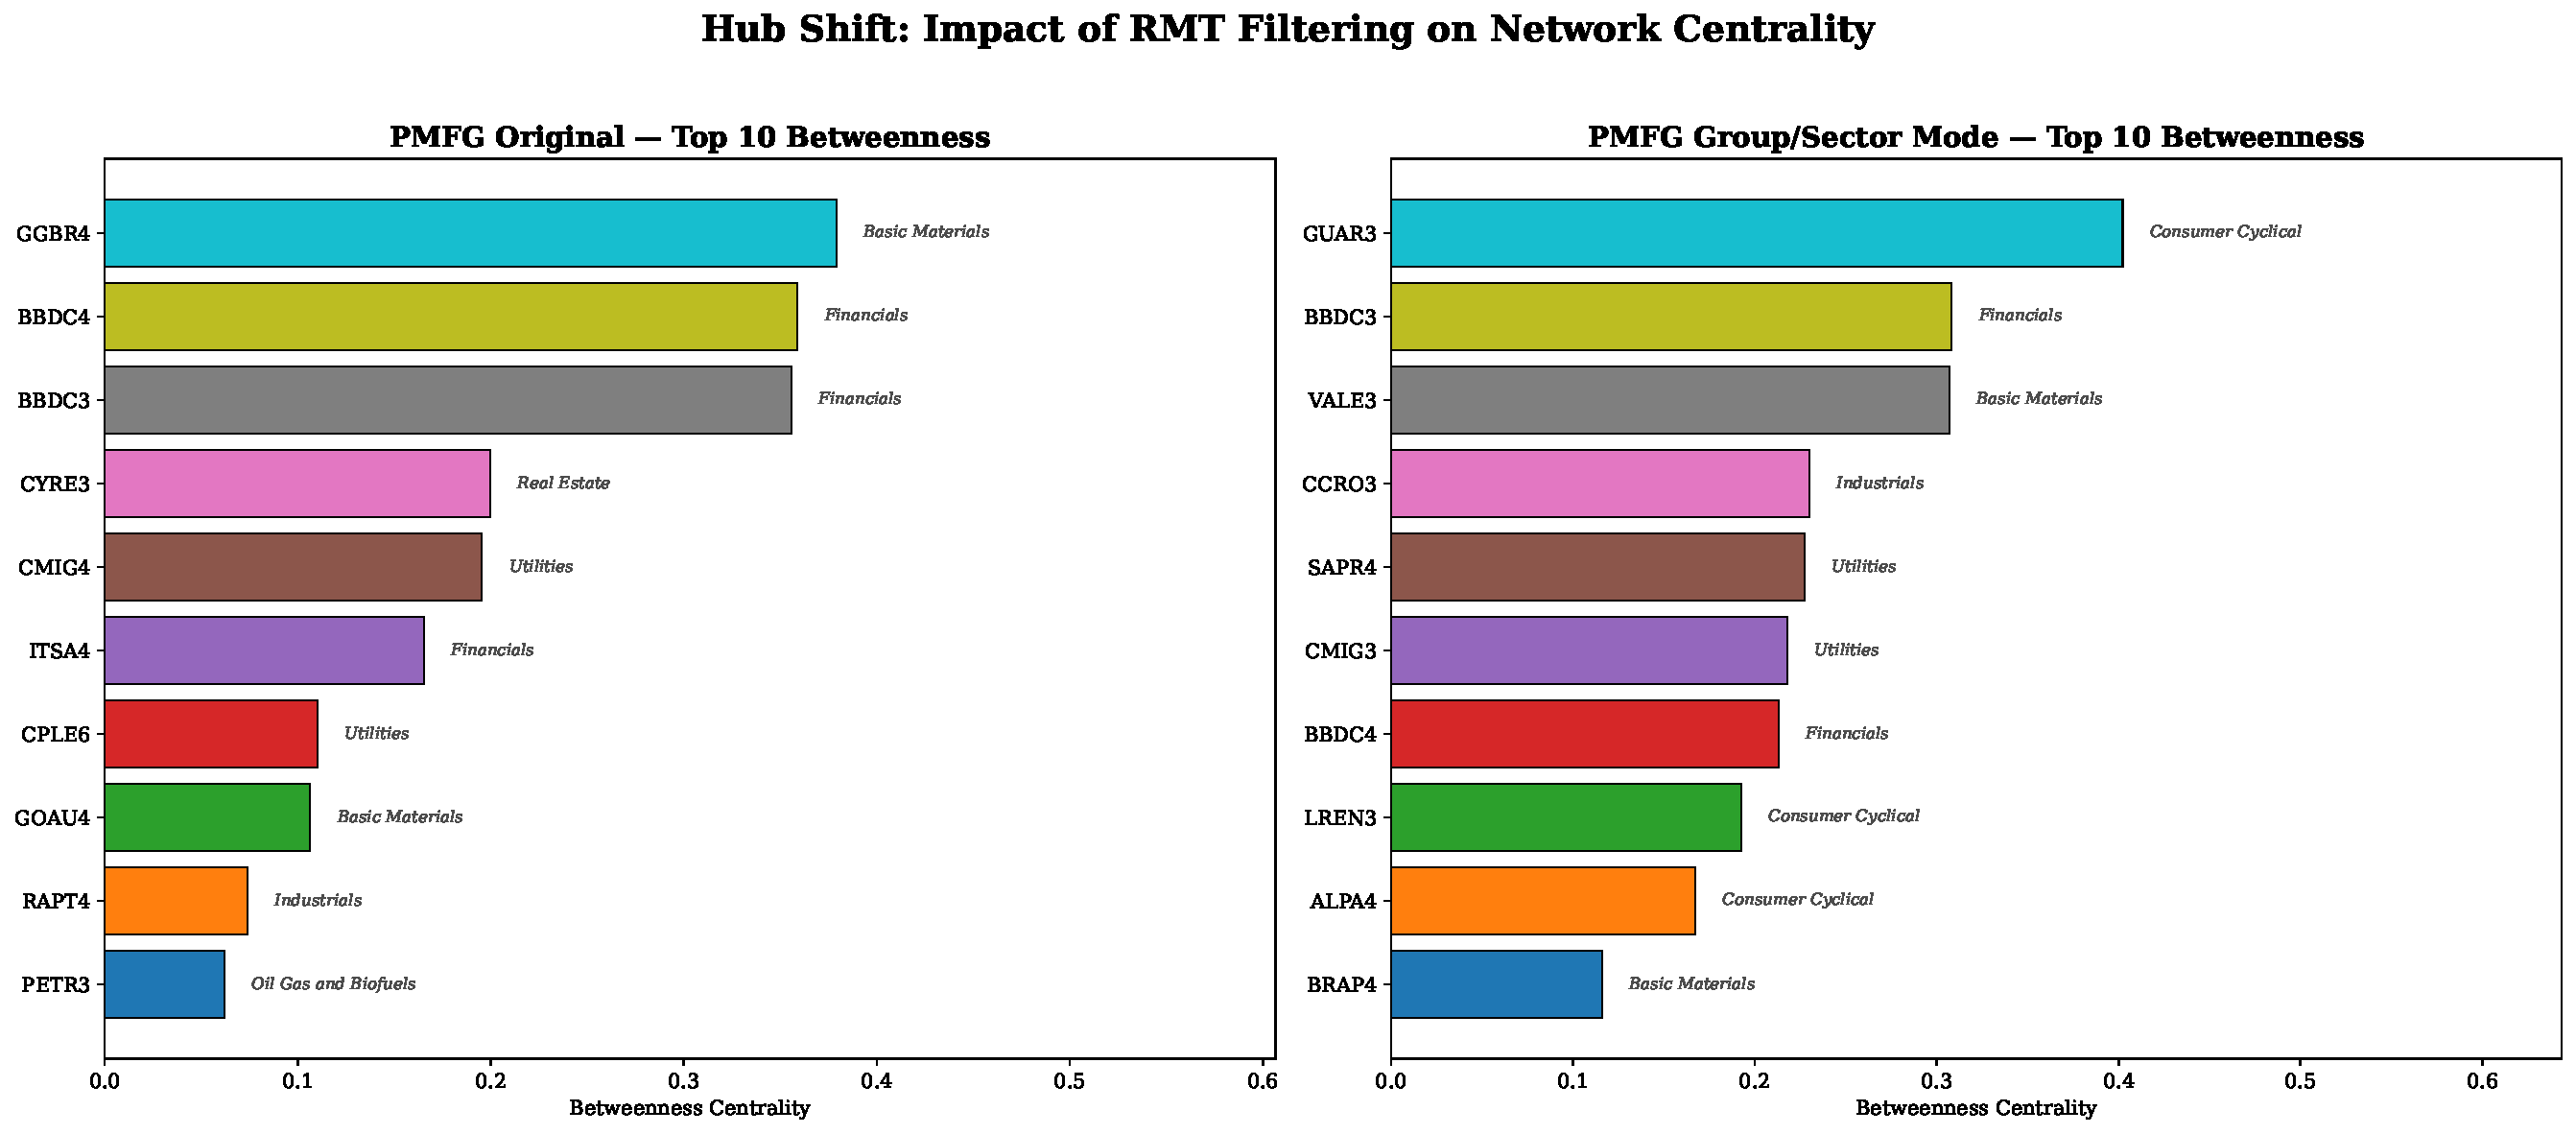
\includegraphics[
width=\linewidth,
height=0.58\textheight,
keepaspectratio
]{images/figure_14_network_hub_rank_comparison.pdf}
\captionof{figure}{Hub-rank comparison across original and group-mode networks. Removal of the dominant market component changes which assets occupy central positions in the dependency structure.}
\label{fig:hub_rank}
\end{center}



\begin{center}
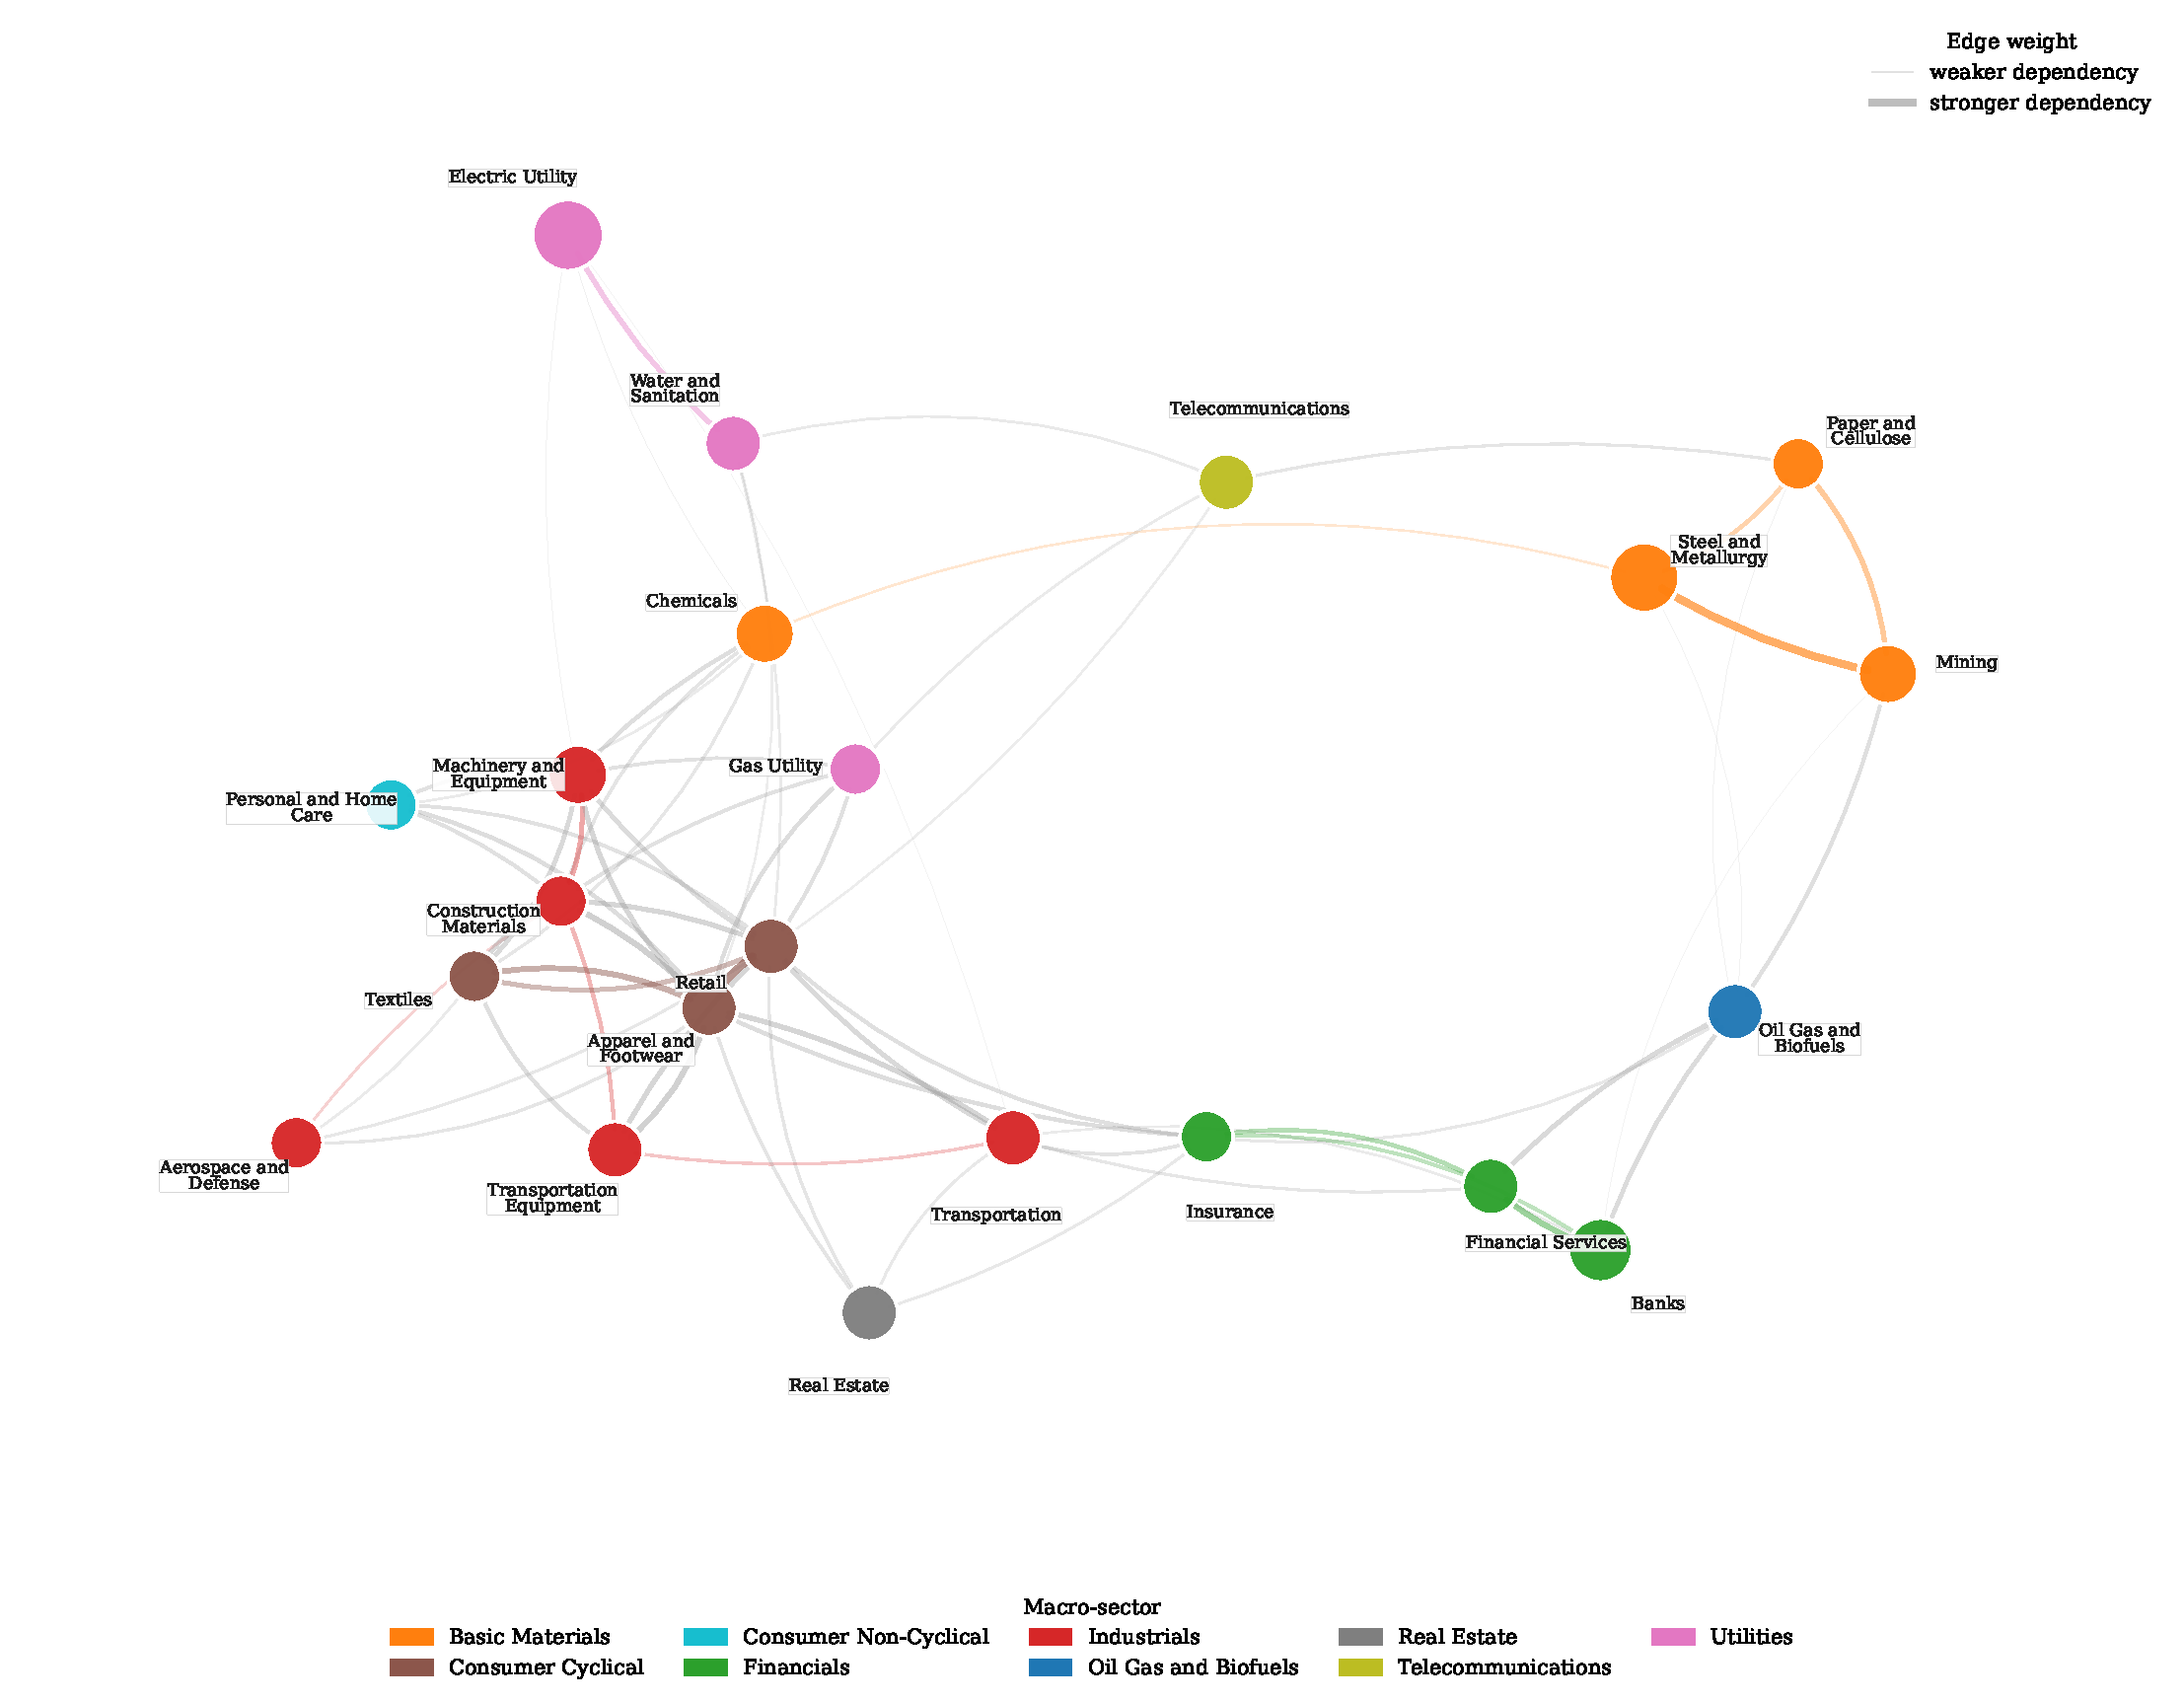
\includegraphics[
width=0.92\linewidth,
height=0.58\textheight,
keepaspectratio
]{images/figure_15_subsector_dependency_network.pdf}
\captionof{figure}{Aggregated subsector dependency network. Nodes represent subsectors, node colour identifies the macro-sector and node size is proportional to the number of assets in each subsector. Edge thickness represents the average retained dependency between connected subsectors.}
\label{fig:subsector_network}
\end{center}

The original-network hubs can reflect both localized relationships and exposure to the broad common component. After market-mode removal, the central nodes instead characterize the residual dependency structure. Assets such as GUAR3, BBDC3, VALE3, CCRO3, SAPR4 and CMIG3 consequently gain prominence in the group-mode rankings. These rankings are interpreted as descriptive full-sample configurations rather than permanent structural labels, since their temporal stability is examined separately in Section~\ref{sec:robustness}.

To translate this ticker-level organization into a more interpretable economic representation, we aggregate the retained dependencies by subsector. The resulting network contains 22 subsectors and 66 undirected links, with density 0.2857. Its mean and median edge dependencies are 0.0566 and 0.0561, respectively. These relatively small values are expected because the graph summarizes dependencies after spectral filtering and aggregation rather than raw pairwise correlations.

Figure~\ref{fig:subsector_network} shows the resulting subsector-level structure. Nodes represent subsectors, node colours indicate macro-sectors, and node sizes reflect the number of constituent assets. Edge thickness represents the average retained dependency between the corresponding subsectors.

The aggregated network reveals different forms of structural importance. Retail has the highest degree, indicating the largest number of retained direct subsector connections. Electric Utility has the highest betweenness, placing it in a bridge-like position between different parts of the graph. Apparel and Footwear has the highest weighted degree, indicating that its retained connections are comparatively strong. These differences show that connectivity, bridging position, and dependency intensity capture distinct aspects of the residual market structure.

The subsector representation therefore provides an economic summary of the organization identified previously at the spectral and ticker-network levels. The analysis begins with non-leading RMT modes, shows that localized structure persists in hierarchical and graph representations, and finally translates the retained network relationships into sectoral and subsector-level organization. This completes the structural part of the empirical analysis before the robustness tests and retrospective volatility-model assessment.


\subsection{Robustness of the Structural Findings}
\label{sec:robustness}

The preceding results identify sectoral organization, significant non-leading spectral modes, and a reorganization of hierarchical and network structure after removal of the dominant market component. We now examine whether these findings remain when key features of the analysis are challenged. The robustness analysis focuses on three potential sensitivities: the economic labels assigned to assets, the presence of multiple share classes from the same issuer, and the stability of the resulting network structure across time.

\subsubsection{Robustness of the Sectoral and Spectral Structure}

The sectoral pattern identified in Section~\ref{sec:stylized_correlation} is tested using an asset-level label-permutation procedure that preserves both the empirical dependency matrix and the observed sector-size distribution. The observed difference between mean within-sector and between-sector correlations is $\Delta_{\mathrm{sector}}=0.1184$, whereas the 95th percentile of the permutation distribution is 0.0245. None of the 10,000 permutations produces a difference as large as the observed value ($p\approx 10^{-4}$, the minimum attainable at this simulation count). The stronger within-sector dependence is therefore not reproduced by random reassignment of the existing sector labels.

A separate robustness concern arises from companies represented by multiple listed share classes. The 58-asset panel contains 12 such issuers, which can strengthen issuer-specific co-movement and generate localized spectral components. We therefore repeat the RMT analysis after retaining one deterministic representative per company, reducing the cross-section to 46 issuers.

\begin{center}
\captionof{table}{Issuer-level RMT robustness check on the same 1,527 dates as the full panel. Parentheses give the number of non-market modes above the Mar\v{c}enko--Pastur upper bound.}
\label{tab:issuer_rmt_robustness}
\small
\resizebox{\linewidth}{!}{%
\begin{tabular}{lrrrrrrr}
\toprule
Panel & $N$ & $T$ & $Q$ & $\lambda_{+}$ & Eigenvalues above $\lambda_{+}$ & $\lambda_{1}/N$ & Mean pairwise corr. \\
\midrule
Full share-class panel & 58 & 1527 & 26.33 & 1.4278 & 5 (4) & 0.3733 & 0.3350 \\
Issuer-collapsed panel & 46 & 1527 & 33.20 & 1.3773 & 3 (2) & 0.3611 & 0.3215 \\
\bottomrule
\end{tabular}}
\end{center}



Both panels use the common dates 23 August 2006--15 August 2024, so this comparison changes the cross-section while holding the observation period fixed. Issuer representatives are selected by common-panel coverage, then mean financial volume over those same dates, then ticker as a deterministic final tie-break. The rule retains PETR4 over PETR3, ELET3 over ELET6, and CPLE6 over CPLE3. The leading trace share is 0.3733 in the full panel and 0.3611 after collapse. Four non-market eigenvalues exceed the full-panel bound, compared with two in the issuer panel (2.2912 and 1.5388). Thus the number of candidate group modes is sensitive to share-class representation even when $T$ is held constant.

The group-mode matrix and both graph families were recomputed for the two panels on these same dates. Table~\ref{tab:issuer_network_robustness} reports the group-mode network summaries; it separates the effect of reducing $N$ from the prior comparison, which also changed $T$.

\begin{center}
\captionof{table}{MST and PMFG summaries for the group-mode matrices recomputed on the same dates.}
\label{tab:issuer_network_robustness}
\small
\resizebox{\linewidth}{!}{%
\begin{tabular}{llrrrrrr}
\toprule
Panel & Network & Assets & Edges & Mean edge corr. & Same-sector ratio & Clustering & Top degree / betweenness \\
\midrule
Full share-class & MST & 58 & 57 & 0.1388 & 0.6316 & 0.0000 & ALPA4 / ALPA4 \\
Issuer-collapsed & MST & 46 & 45 & 0.0982 & 0.6000 & 0.0000 & CMIG4 / SHUL4 \\
Full share-class & PMFG & 58 & 168 & 0.1109 & 0.5417 & 0.6653 & GUAR3 / GUAR3 \\
Issuer-collapsed & PMFG & 46 & 132 & 0.0812 & 0.4621 & 0.6761 & ROMI3 / SAPR4 \\
\bottomrule
\end{tabular}}
\end{center}



After issuer collapse, mean group-mode edge correlation decreases for both the MST and PMFG, while PMFG average clustering is similar. The edge counts equal $N-1$ and $3N-6$, respectively, in each panel. These changes describe sensitivity to cross-sectional composition; the analysis does not attribute them to a change in sample dates.

We further test the spectral results against a circular-shift surrogate null. Each surrogate preserves the marginal distribution and temporal ordering of every individual return series while breaking their contemporaneous alignment across assets. Across 1,000 independent surrogate realizations, empirical ranks 1--5 exceed their rank-matched 95th-percentile thresholds. Rank 6 is the first that does not: its empirical value is 1.1673, below the null 95th percentile of 1.3057; ranks 6--58 have 1,000 of 1,000 surrogate values at least as large as the empirical value ($p=1$ under the plus-one estimate). For ranks 1--5, zero exceedances give $p=1/(1,001)\approx0.001$, the minimum attainable. This identifies where the empirical spectrum ceases to exceed the circular-shift null.

The issuer-collapse and circular-shift results should be interpreted jointly. The surrogate experiment supports the presence of genuine cross-sectional synchronization beyond the null benchmark, whereas the issuer-level experiment shows that the economic interpretation of some weaker modes remains sensitive to the representation of multiple share classes. Robust statistical separation from the null therefore does not imply that every significant mode corresponds to a broad or stable economic factor.

\subsubsection{Temporal Stability of the Network Structure}

The full-sample MST and PMFG representations summarize long-run dependency structure, but their individual edges and central nodes need not remain unchanged through time. To examine this sensitivity, the synchronized sample is divided into three consecutive windows of 509 observations and the networks are re-estimated within each window. Table~\ref{tab:network_temporal_stability} summarizes the mean pairwise overlap across the resulting network realizations.

\begin{center}
\captionof{table}{Temporal stability of the MST and PMFG structures across three consecutive windows. Values are means across window pairs.}
\label{tab:network_temporal_stability}

\small
\begin{tabular}{llrrr}
\toprule
Network & Matrix & Edge Jaccard & Top-5 hub overlap & Community ARI \\
\midrule
MST & Original & 0.206 & 0.267 & 0.138 \\
MST & Group mode & 0.047 & 0.200 & 0.182 \\
PMFG & Original & 0.212 & 0.200 & 0.214 \\
PMFG & Group mode & 0.140 & 0.200 & 0.174 \\
\bottomrule
\end{tabular}
\end{center}



Edge persistence is modest in the original networks and lower still for several group-mode comparisons. The mean edge Jaccard similarity is 0.206 for the original MST and 0.212 for the original PMFG, compared with 0.047 and 0.140 for their group-mode counterparts. Hub persistence is also limited: mean overlap among the five highest-betweenness nodes ranges from 0.20 to 0.27, and no top-five betweenness hub appears in all three windows. Community agreement, measured by the adjusted Rand index, is similarly modest.

These results qualify the interpretation of the full-sample networks. The structural analyses in Section~\ref{sec:network_organization} identify meaningful long-run dependency configurations, but individual edges, hub identities, and community assignments should not be interpreted as invariant properties of the Brazilian equity market. This distinction is particularly important for the retrospective volatility assessment that follows, where full-sample structural descriptors are used as ex-post characteristics rather than as point-in-time network estimates.


\subsection{Retrospective Volatility-Model Assessment}
\label{sec:forecasting}

The preceding analyses identify cross-sectional dependency structure in B3 equities. We now ask whether adding structural descriptors improves realized-volatility forecast accuracy. The RMT and network descriptors are estimated from the full synchronized sample, so this is a retrospective comparison rather than a point-in-time forecasting design.

The chronological test period is 2021--2025. Specifications are selected by mean validation QLIKE within each model family and feature set; no test-period metric is used for selection. Figure~\ref{fig:forecast_comparison} shows aggregated test QLIKE. Lower values indicate lower loss. The confidence intervals are circular moving-block bootstrap intervals and are descriptive; paired HAC tests provide the focused feature-set comparisons below.

\begin{center}
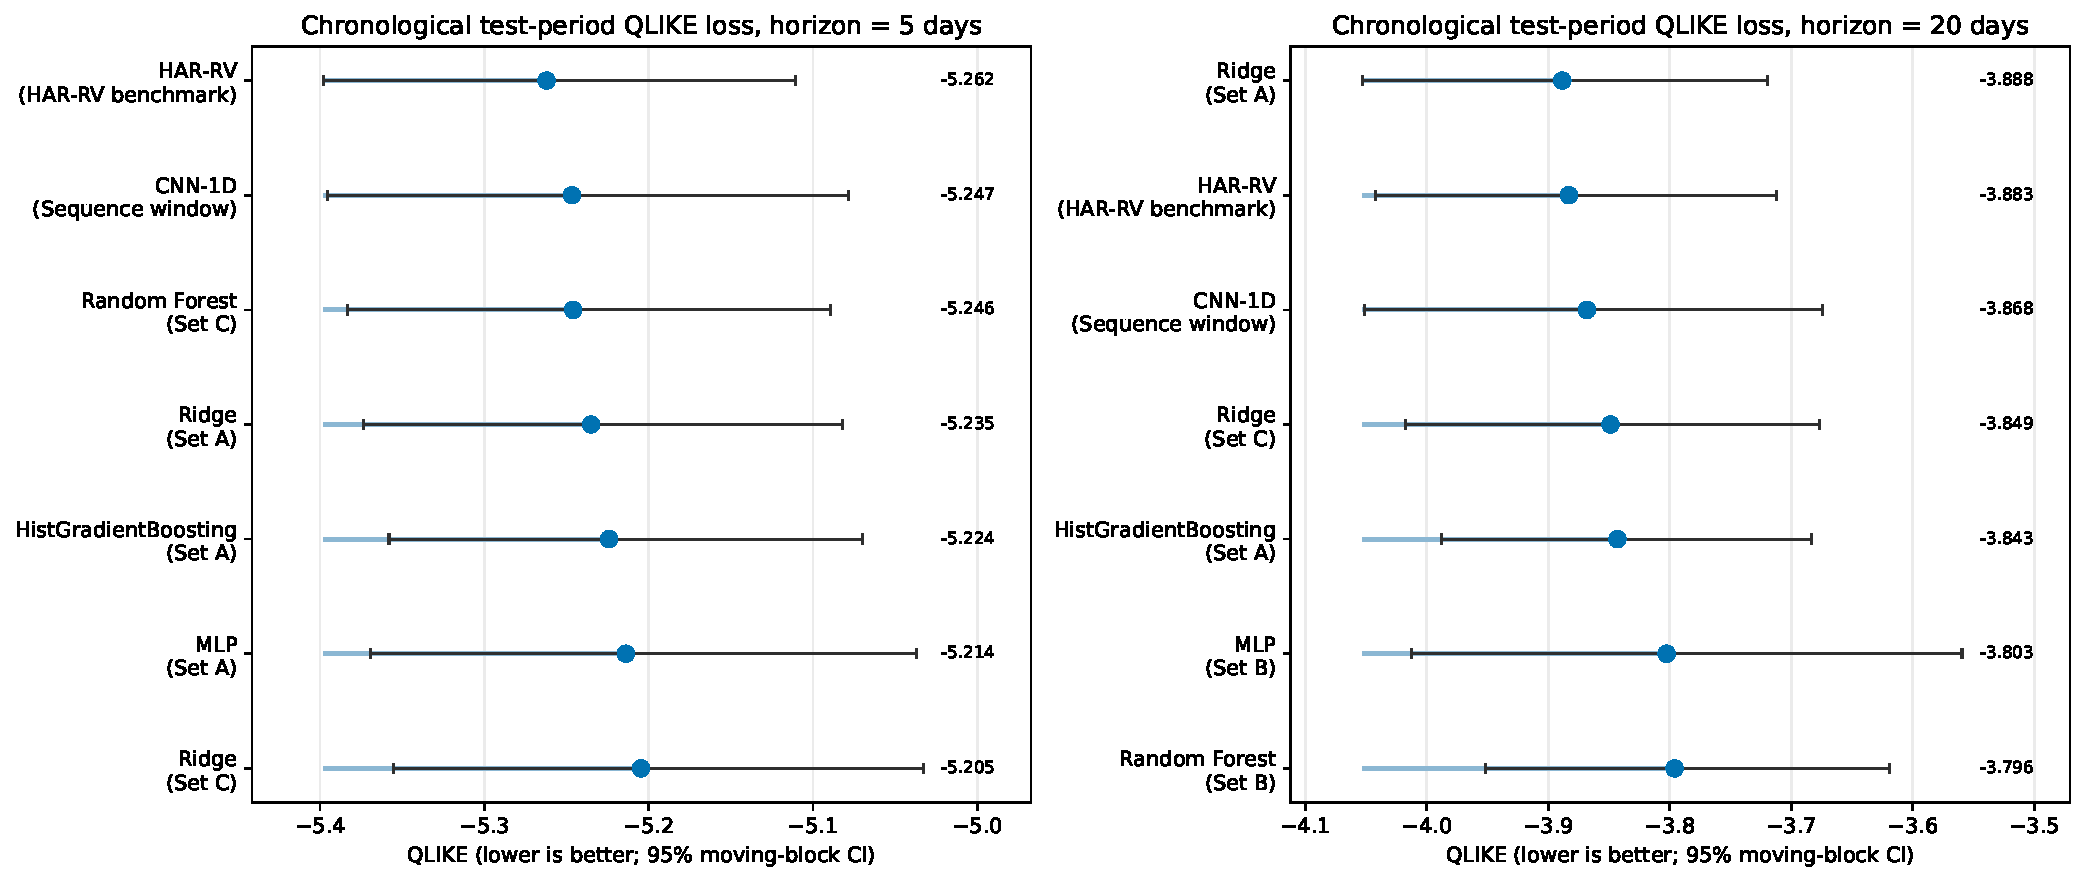
\includegraphics[width=\linewidth,height=0.58\textheight,keepaspectratio]{images/figure_16_volatility_forecast_model_comparison.pdf}
\captionof{figure}{Chronological test-period QLIKE across validation-selected specifications. Points show the mean across PETR4, VALE3 and BBDC4; bars show 95\% circular moving-block bootstrap intervals from 2,000 replications, with block length equal to the forecast horizon.}
\label{fig:forecast_comparison}
\end{center}

HAR-RV has the lowest mean QLIKE at the 5-day horizon; at 20 days, the explicit Ridge Set A comparator has a slightly lower mean than HAR-RV. The bootstrap intervals overlap substantially, so these descriptive rankings do not establish that either specification is significantly better than every alternative. The primary structural comparison is between validation-selected Ridge Set A and Ridge Set B/C, because these specifications isolate the addition of market/RMT and network descriptors while keeping the model family fixed.

Table~\ref{tab:forecast_comparison} gives validation-selected test summaries, the explicit Ridge Set A comparator, and HAR-RV. The asset-level results, block-length sensitivity and five-seed neural sensitivity are reported in Tables~\ref{tab:app_forecast},~\ref{tab:app_blocks} and~\ref{tab:app_seeds}.

\begin{center}
\captionof{table}{Validation-selected model results and the fixed Ridge Set A comparator on the 2021--2025 test period. Metrics are averaged across PETR4, VALE3 and BBDC4.}
\label{tab:forecast_comparison}
\resizebox{\linewidth}{!}{%
\begin{tabular}{lllrrrrr}
\toprule
Horizon & Model & Feature set & MAE & RMSE & QLIKE & 95\% CI for QLIKE & $R^2_{\mathrm{oos}}$ \\
\midrule
5 & CNN-1D & Sequence window & 0.0145 & 0.0213 & $-5.2467$ & $[-5.3955, -5.0784]$ & 0.2871 \\
5 & Random Forest & Set C (+Network) & 0.0162 & 0.0227 & $-5.2460$ & $[-5.3834, -5.0895]$ & 0.2001 \\
5 & HistGradientBoosting & Set A (Classical) & 0.0168 & 0.0235 & $-5.2241$ & $[-5.3581, -5.0700]$ & 0.1468 \\
5 & MLP & Set A (Classical) & 0.0138 & 0.0209 & $-5.2139$ & $[-5.3692, -5.0369]$ & 0.3150 \\
5 & Ridge & Set C (+Network) & 0.0146 & 0.0215 & $-5.2047$ & $[-5.3553, -5.0329]$ & 0.2733 \\
20 & CNN-1D & Sequence window & 0.0210 & 0.0308 & $-3.8682$ & $[-4.0509, -3.6740]$ & 0.3947 \\
20 & Ridge & Set C (+Network) & 0.0224 & 0.0316 & $-3.8487$ & $[-4.0177, -3.6765]$ & 0.3587 \\
20 & HistGradientBoosting & Set A (Classical) & 0.0265 & 0.0375 & $-3.8430$ & $[-3.9879, -3.6834]$ & 0.1560 \\
20 & MLP & Set B (+Market/RMT) & 0.0220 & 0.0322 & $-3.8026$ & $[-4.0126, -3.5595]$ & 0.3514 \\
20 & Random Forest & Set B (+Market/RMT) & 0.0284 & 0.0405 & $-3.7960$ & $[-3.9514, -3.6195]$ & 0.0124 \\
5 & Ridge (Set A baseline) & Set A (Classical) & 0.0146 & 0.0213 & $-5.2351$ & $[-5.3736, -5.0820]$ & 0.2813 \\
5 & HAR-RV & HAR-RV benchmark & 0.0157 & 0.0222 & $-5.2622$ & $[-5.3978, -5.1109]$ & 0.2228 \\
20 & Ridge (Set A baseline) & Set A (Classical) & 0.0217 & 0.0306 & $-3.8884$ & $[-4.0528, -3.7198]$ & 0.3941 \\
20 & HAR-RV & HAR-RV benchmark & 0.0240 & 0.0335 & $-3.8830$ & $[-4.0422, -3.7123]$ & 0.2826 \\
\bottomrule
\end{tabular}}
\end{center}

\noindent\footnotesize\emph{Notes:} QLIKE is defined in Eq.~\eqref{eq:theory_qlike}; $R^2_{\mathrm{oos}}$ is relative to the training-sample mean benchmark. Set A contains point-in-time return and volatility predictors; Set B adds market and full-sample RMT descriptors; Set C additionally includes full-sample MST and PMFG descriptors. Sets B and C are retrospective structural specifications.
\normalsize

We compare validation-selected Ridge Set B/C with Ridge Set A using date-level mean QLIKE differences across the three assets and Newey--West standard errors with horizon-specific lags. The same test also reports HAR-RV versus Ridge Set A. The difference is defined as baseline QLIKE minus candidate QLIKE, so a positive value favours the candidate. Table~\ref{tab:forecast_loss_test} reports two-sided $p$-values; Holm adjustment is applied across the four structural contrasts.

\begin{center}
\captionof{table}{HAC tests of validation-selected feature-set contrasts and HAR-RV against Ridge Set A. Negative differences favour the Set A baseline.}
\label{tab:forecast_loss_test}
\resizebox{\linewidth}{!}{%
\begin{tabular}{rlrrrrrr}
\toprule
Horizon & Contrast & Mean difference & HAC s.e. & Statistic & Two-sided $p$ & Holm $p$ \\
\midrule
5 & Set B vs Set A & -0.023021 & 0.006010 & -3.831 & 0.000128 & 0.000384 \\
5 & Set C vs Set A & -0.030401 & 0.007332 & -4.147 & 0.000034 & 0.000135 \\
20 & Set B vs Set A & -0.029578 & 0.010914 & -2.710 & 0.006727 & 0.006727 \\
20 & Set C vs Set A & -0.039761 & 0.011464 & -3.468 & 0.000524 & 0.001047 \\
5 & HAR-RV vs Ridge A & -0.027097 & 0.015080 & -1.797 & 0.072348 & -- \\
20 & HAR-RV vs Ridge A & 0.005454 & 0.011444 & 0.477 & 0.633657 & -- \\
\bottomrule
\end{tabular}}
\end{center}

\noindent\footnotesize\emph{Notes:} The loss difference is QLIKE$_{\mathrm{Ridge\ A}}-$QLIKE$_{\mathrm{candidate}}$, averaged by date across the three assets. Newey--West lags are 4 and 19 for the 5- and 20-day horizons. Holm adjustment covers the four Set B/C versus Set A tests; HAR-RV contrasts are shown separately and are not included in that family.
\normalsize

All four Ridge Set B/C contrasts have negative mean differences, and their two-sided HAC tests remain significant after Holm adjustment. Thus, in this retrospective test, adding the structural feature sets does not improve QLIKE over Ridge Set A; the observed losses are higher. The HAR-RV versus Ridge Set A comparison is not significant at either horizon. These results answer the accuracy question for the evaluated pooled assets and split, but do not establish performance for recursively estimated, point-in-time structural features.

\begin{center}
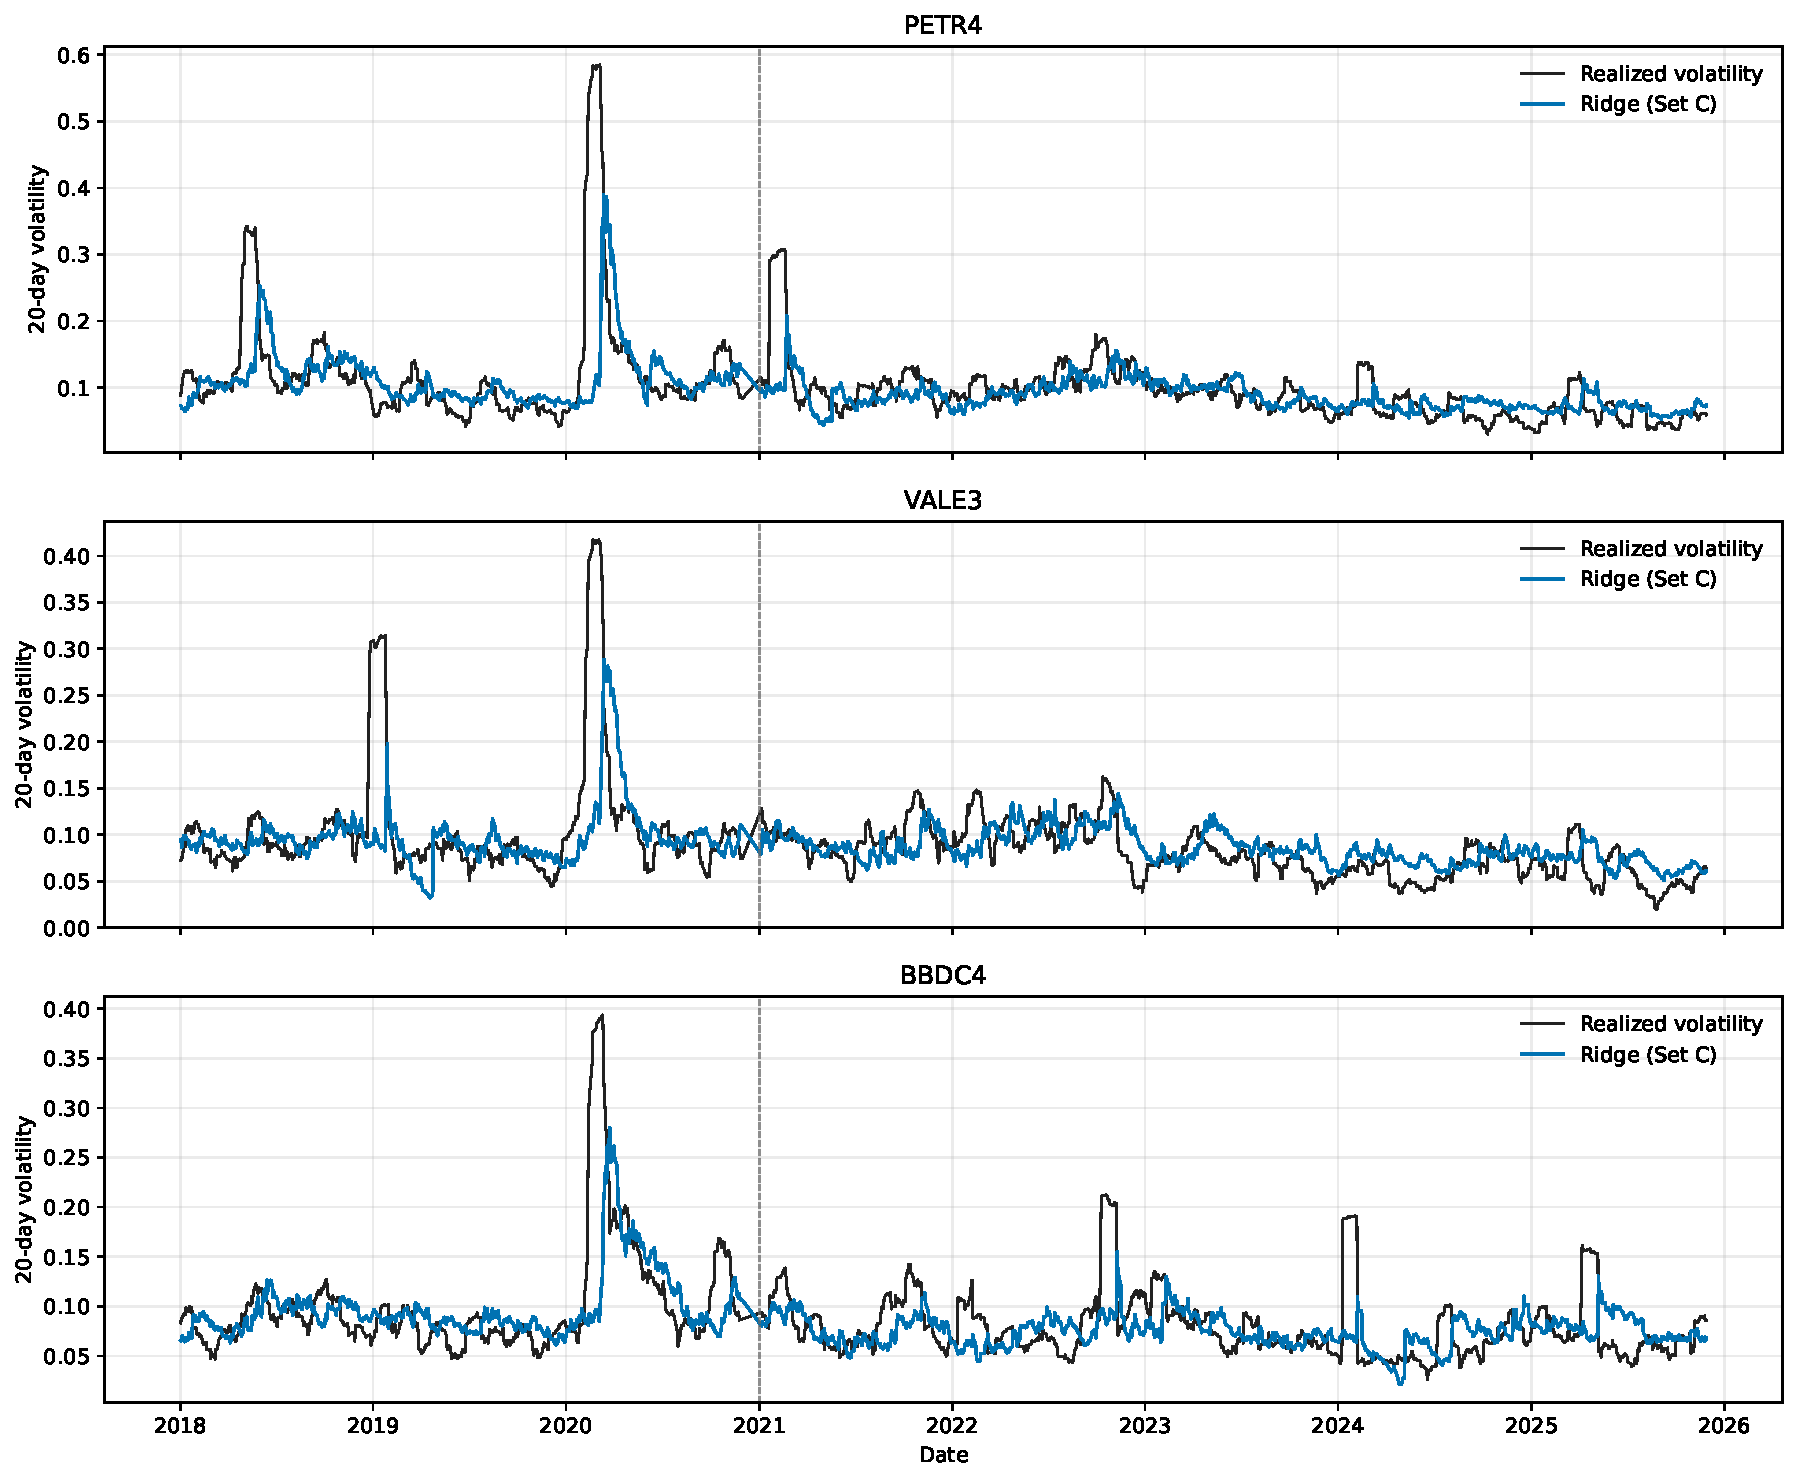
\includegraphics[width=0.95\linewidth,height=0.58\textheight,keepaspectratio]{images/figure_17_realized_vs_predicted_volatility.pdf}
\captionof{figure}{Realized and predicted 20-day volatility for PETR4, VALE3 and BBDC4 using the specification selected on validation data. The vertical dashed line marks the beginning of the 2021--2025 test period.}
\label{fig:realized_vs_predicted}
\end{center}

Figure~\ref{fig:realized_vs_predicted} shows that forecasts follow persistent volatility changes but smooth abrupt realized spikes and subsequent reversals. This visual pattern complements, but does not replace, the aggregate loss comparisons.

Figure~\ref{fig:feature_importance} reports the largest Random Forest impurity-based importance entries across candidate feature sets at each horizon. These values describe how fitted trees use predictors; they do not estimate marginal forecast gains or causal contributions.

\begin{center}
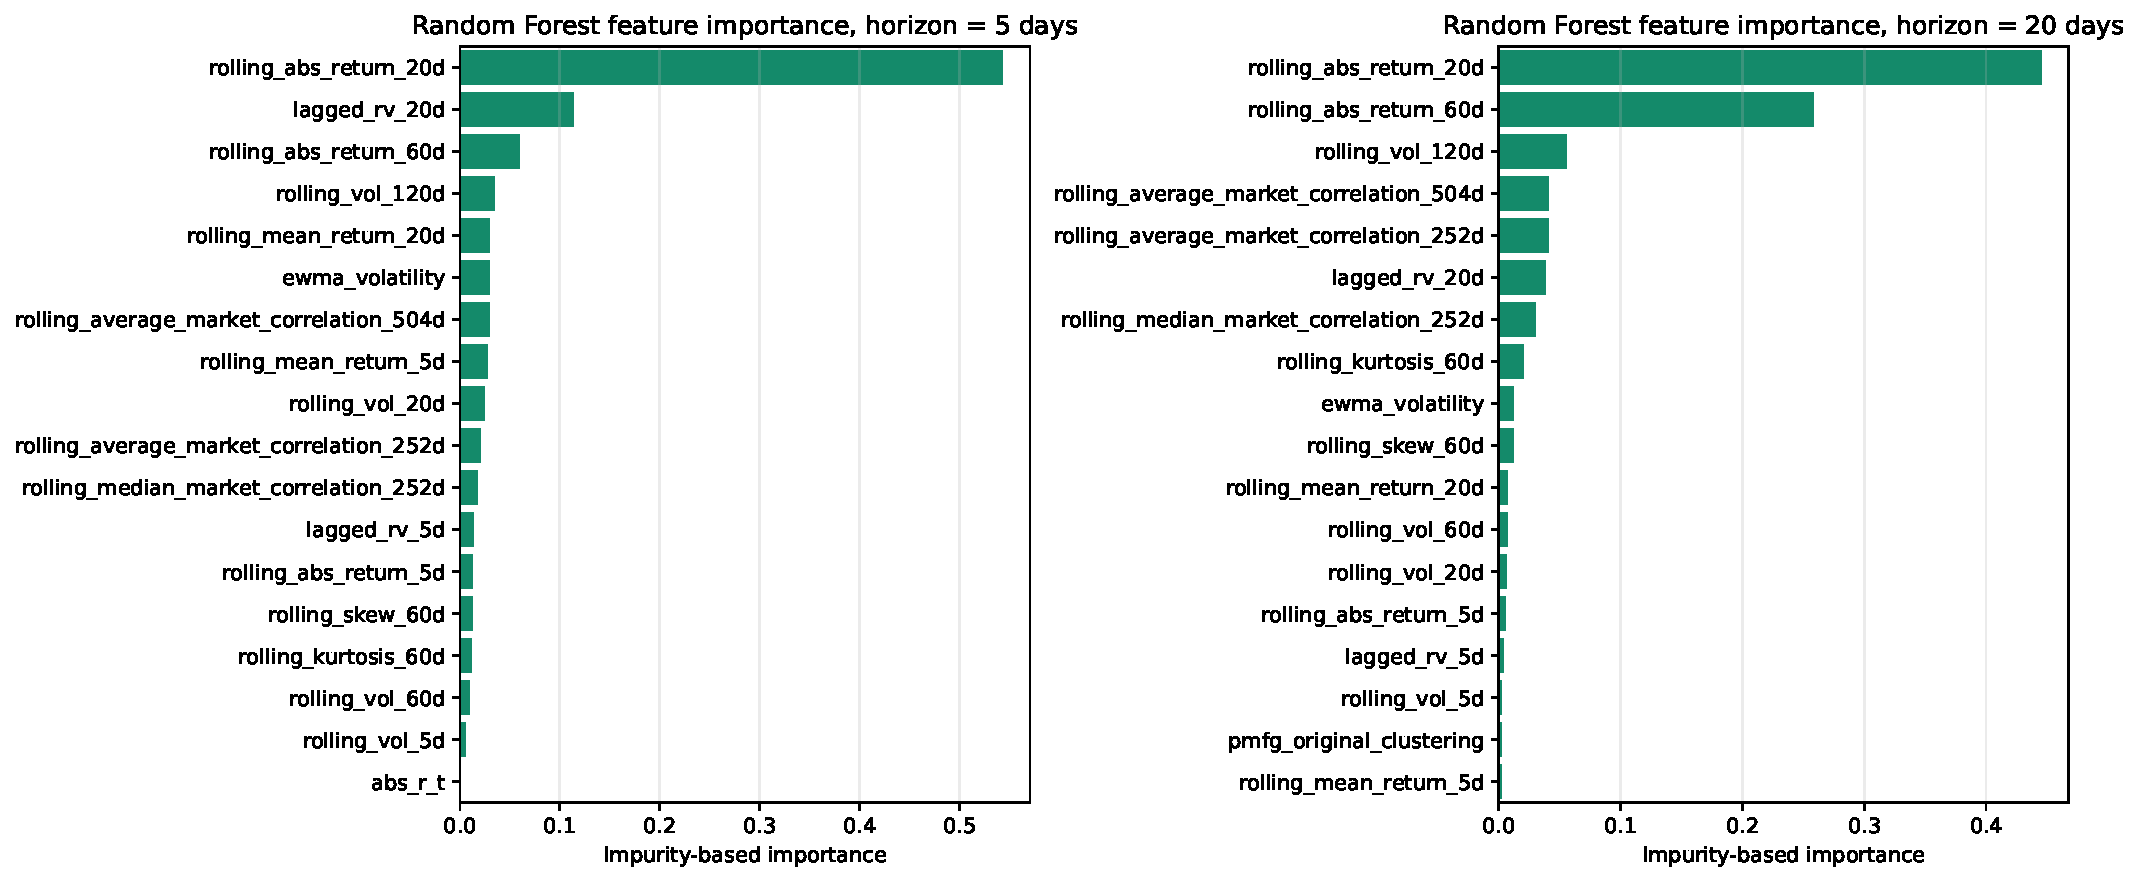
\includegraphics[width=0.95\linewidth,height=0.58\textheight,keepaspectratio]{images/figure_18_ml_feature_importance.pdf}
\captionof{figure}{Random Forest impurity-based importance for the validation-selected feature set at each horizon. Importance is descriptive and is not a measure of incremental predictive value.}
\label{fig:feature_importance}
\end{center}

Conventional volatility predictors account for most of the highest-ranked entries. Structural descriptors also appear in selected models, but their presence among tree splits does not override the test result: the paired Ridge comparisons do not show an accuracy gain from Set B or Set C. Neural-seed sensitivity and block-length sensitivity are documented in Tables~\ref{tab:app_seeds} and~\ref{tab:app_blocks}.



\section{Discussion}
\label{sec:discussion}

The results support a layered interpretation of dependency structure in the Brazilian equity market, consistent with the multi-scale perspective discussed by Raddant and Di Matteo~\cite{raddant_dimatteo_2023}. At the broadest scale, the market exhibits a strong collective component. Positive average cross-correlation, periods of increased market-wide synchronization and the dominant leading eigenvalue all point to a common mode affecting a large part of the equity universe. This collective component is important because it can dominate raw correlation-based representations and obscure weaker relationships operating at more localized scales.

Beyond this market-wide component, the results reveal additional structure that cannot be reduced to simple sector classifications. Within-sector correlations are systematically stronger than between-sector correlations, while the non-leading significant eigenvectors contain recognizable but heterogeneous contrasts involving commodity-related firms, financial institutions, utilities and issuer-specific effects. The spectral results therefore suggest that intermediate-scale organization exists, but that it does not necessarily coincide with predefined economic sectors. This distinction is important when interpreting financial dependencies: statistically significant collective modes may reflect combinations of economic, institutional and issuer-specific relationships rather than isolated sector factors.

The hierarchical and network representations provide complementary evidence for this interpretation. After removal of the dominant market mode, the remaining dependency structure becomes weaker in absolute correlation terms but does not disappear. Ordered heatmaps and hierarchical clustering continue to reveal localized organization, while the lower cophenetic correlation of the group-mode representation suggests that this residual geometry is less purely tree-like. The MST and PMFG therefore add information by retaining different aspects of the dependency structure beyond a strictly hierarchical representation.

The PMFG results are particularly informative in this respect. Market-mode removal substantially reduces average edge strength, yet local clustering increases in the group-mode network. This combination indicates that weaker pairwise dependencies can still form relatively concentrated local structures once broad market synchronization is removed. The result is consistent with the role of planar filtering as a way to preserve richer local organization than the MST alone \cite{tumminello_2005_tool,tumminello_2010_correlation}. Hub reorganization further reinforces this interpretation: assets that are central in the original network are not necessarily the same assets that become central after removal of the collective component. Network centrality should therefore be understood as conditional on the dependency representation from which the graph is constructed.

The subsector-level network provides an economic summary of this residual organization. Differences between degree, weighted degree and betweenness show that connectivity, dependency intensity and bridge-like position describe distinct aspects of market structure. At the same time, the robustness results caution against interpreting these configurations as permanent characteristics. The dominant spectral component remains identifiable after collapsing multiple share classes to the issuer level, and the leading empirical eigenvalues remain distinguishable from the circular-shift surrogate benchmark. However, weaker modes are more sensitive to issuer representation, while individual network edges, hubs and communities show limited persistence across time windows. The full-sample networks should therefore be interpreted as long-run structural summaries rather than invariant market architectures.

The validation-selected Ridge comparisons show higher test QLIKE for Set B and Set C than for Set A at both horizons; date-level HAC tests favor Set A, including after Holm adjustment across the four structural contrasts. This result is specific to the selected Ridge comparisons and should not be generalized to every model or to a point-in-time deployment. HAR-RV is competitive: its paired comparison with Ridge Set A is not statistically distinguishable at the 5% level. Five-seed sensitivity shows greater QLIKE dispersion for MLP than CNN, so single-seed neural rankings are uncertain. Structural descriptors remain ex-post because they were computed from the full sample.

Overall, the study integrates spectral filtering, hierarchical organization and financial networks to characterize B3 equity dependencies, then evaluates whether adding these descriptors improves volatility forecasts. The Ridge loss comparisons indicate worse test QLIKE after adding market/RMT or network descriptors under this design; HAR and seed-sensitivity results provide relevant context. These results do not establish causal effects or real-time forecasting performance.

The findings should be interpreted in light of several limitations. First, the RMT and network descriptors used in the volatility assessment are estimated from the full synchronized sample and are therefore unavailable at historical forecast origins. The forecasting experiment should consequently be interpreted as a retrospective structural assessment rather than as a strict point-in-time test. The most important extension is to reconstruct the spectral and network descriptors recursively using rolling or expanding windows.

Second, the volatility assessment is restricted to PETR4, VALE3 and BBDC4. Although these assets provide liquid and economically distinct forecasting targets, they do not represent the full B3 cross-section. Extending the experiment to a broader set of assets would provide a stronger assessment of whether the observed relationships generalize across sectors, liquidity profiles and market conditions.

Third, long historical equity samples remain sensitive to data-quality issues associated with corporate actions, ticker transitions, share-class changes and adjustment procedures. Adjusted prices reduce these problems but do not eliminate them entirely. The issuer-level robustness analysis also shows that multiple listed share classes can materially affect some localized spectral components.

Fourth, sector and subsector classifications provide a useful economic reference but remain descriptive labels rather than complete representations of firm exposure. Companies may share dependencies through macroeconomic, liquidity or balance-sheet channels that do not align with predefined classifications. The network and eigenvector results should therefore not be interpreted as causal mappings of economic transmission mechanisms.

Finally, the 1998--2025 local extraction has not been redistributed, and its source-specific license was not verified here; the public BovDBv2 deposit ends in July 2024. Exact reproduction of the local 2025 extension requires authorized data access. The present analysis also relies on static full-sample structural descriptors and relatively simple machine-learning and neural architectures. The study does not establish causal effects of network position on future volatility, nor does it evaluate whether more sophisticated temporal or graph-based models would benefit from dynamically reconstructed network information. Future work should combine point-in-time RMT and network estimation with broader target coverage, alternative rolling-window specifications and models capable of jointly representing temporal and cross-sectional market dynamics.


\section{Conclusions}
\label{sec:conclusion}

This study examined the dependency structure of Brazilian equities traded on B3 through an integrated econophysics framework combining correlation analysis, Random Matrix Theory, hierarchical representations, filtered financial networks, and a retrospective volatility-model assessment. The empirical evidence shows that the Brazilian equity market exhibits positive but heterogeneous cross-sectional dependence, with stronger relationships within economic sectors and substantial variation in market-wide synchronization over time.

The spectral analysis shows that this dependence is strongly influenced by a dominant collective market component, while additional significant modes retain more localized patterns that do not map directly onto simple sector classifications. Removing the leading market mode changes the geometry of the dependency structure rather than eliminating it. Hierarchical clustering, MST, and PMFG representations show that weaker but organized relationships remain, with changes in local clustering, network connectivity, and the identity of central assets. The subsector-level representation further translates these residual dependencies into an economically interpretable view of the market.

In the validation-selected Ridge comparisons, Set B and Set C have higher test QLIKE than Set A at both horizons, and the paired HAC tests favor the Set A baseline after adjustment across the four structural contrasts. HAR-RV also provides an explicit benchmark; its paired comparison with Ridge Set A is not statistically distinguishable at the 5% level. The neural sensitivity analysis shows materially greater seed variation for MLP than for CNN. Because the structural descriptors use the full synchronized sample, these findings are retrospective and do not establish a point-in-time forecasting effect.

The study integrates spectral filtering and network representations to examine broad market synchronization and localized dependency structure in Brazilian equities. A next step is to reconstruct RMT and network descriptors recursively at each forecast origin and test them using only information available at that time.


\appendix
\section{Supplementary figures}
\label{app:supplementary_figures}

% Supplementary figures reserved for additional versions that may be moved
% out of the main text in a later shortened submission draft.
% Candidates: full top-eigenvector loading figure, original MST/PMFG rough
% comparison figures, selected body figures after narrative shortening.

Additional figures and tables generated by the computational workflow are retained as supplementary material. These include asset-universe tables, return summaries, correlation matrices, RMT eigenvector loadings, network edge lists, clique lists, centrality rankings and detailed forecasting results by asset, horizon, model and feature set.

\begin{center}
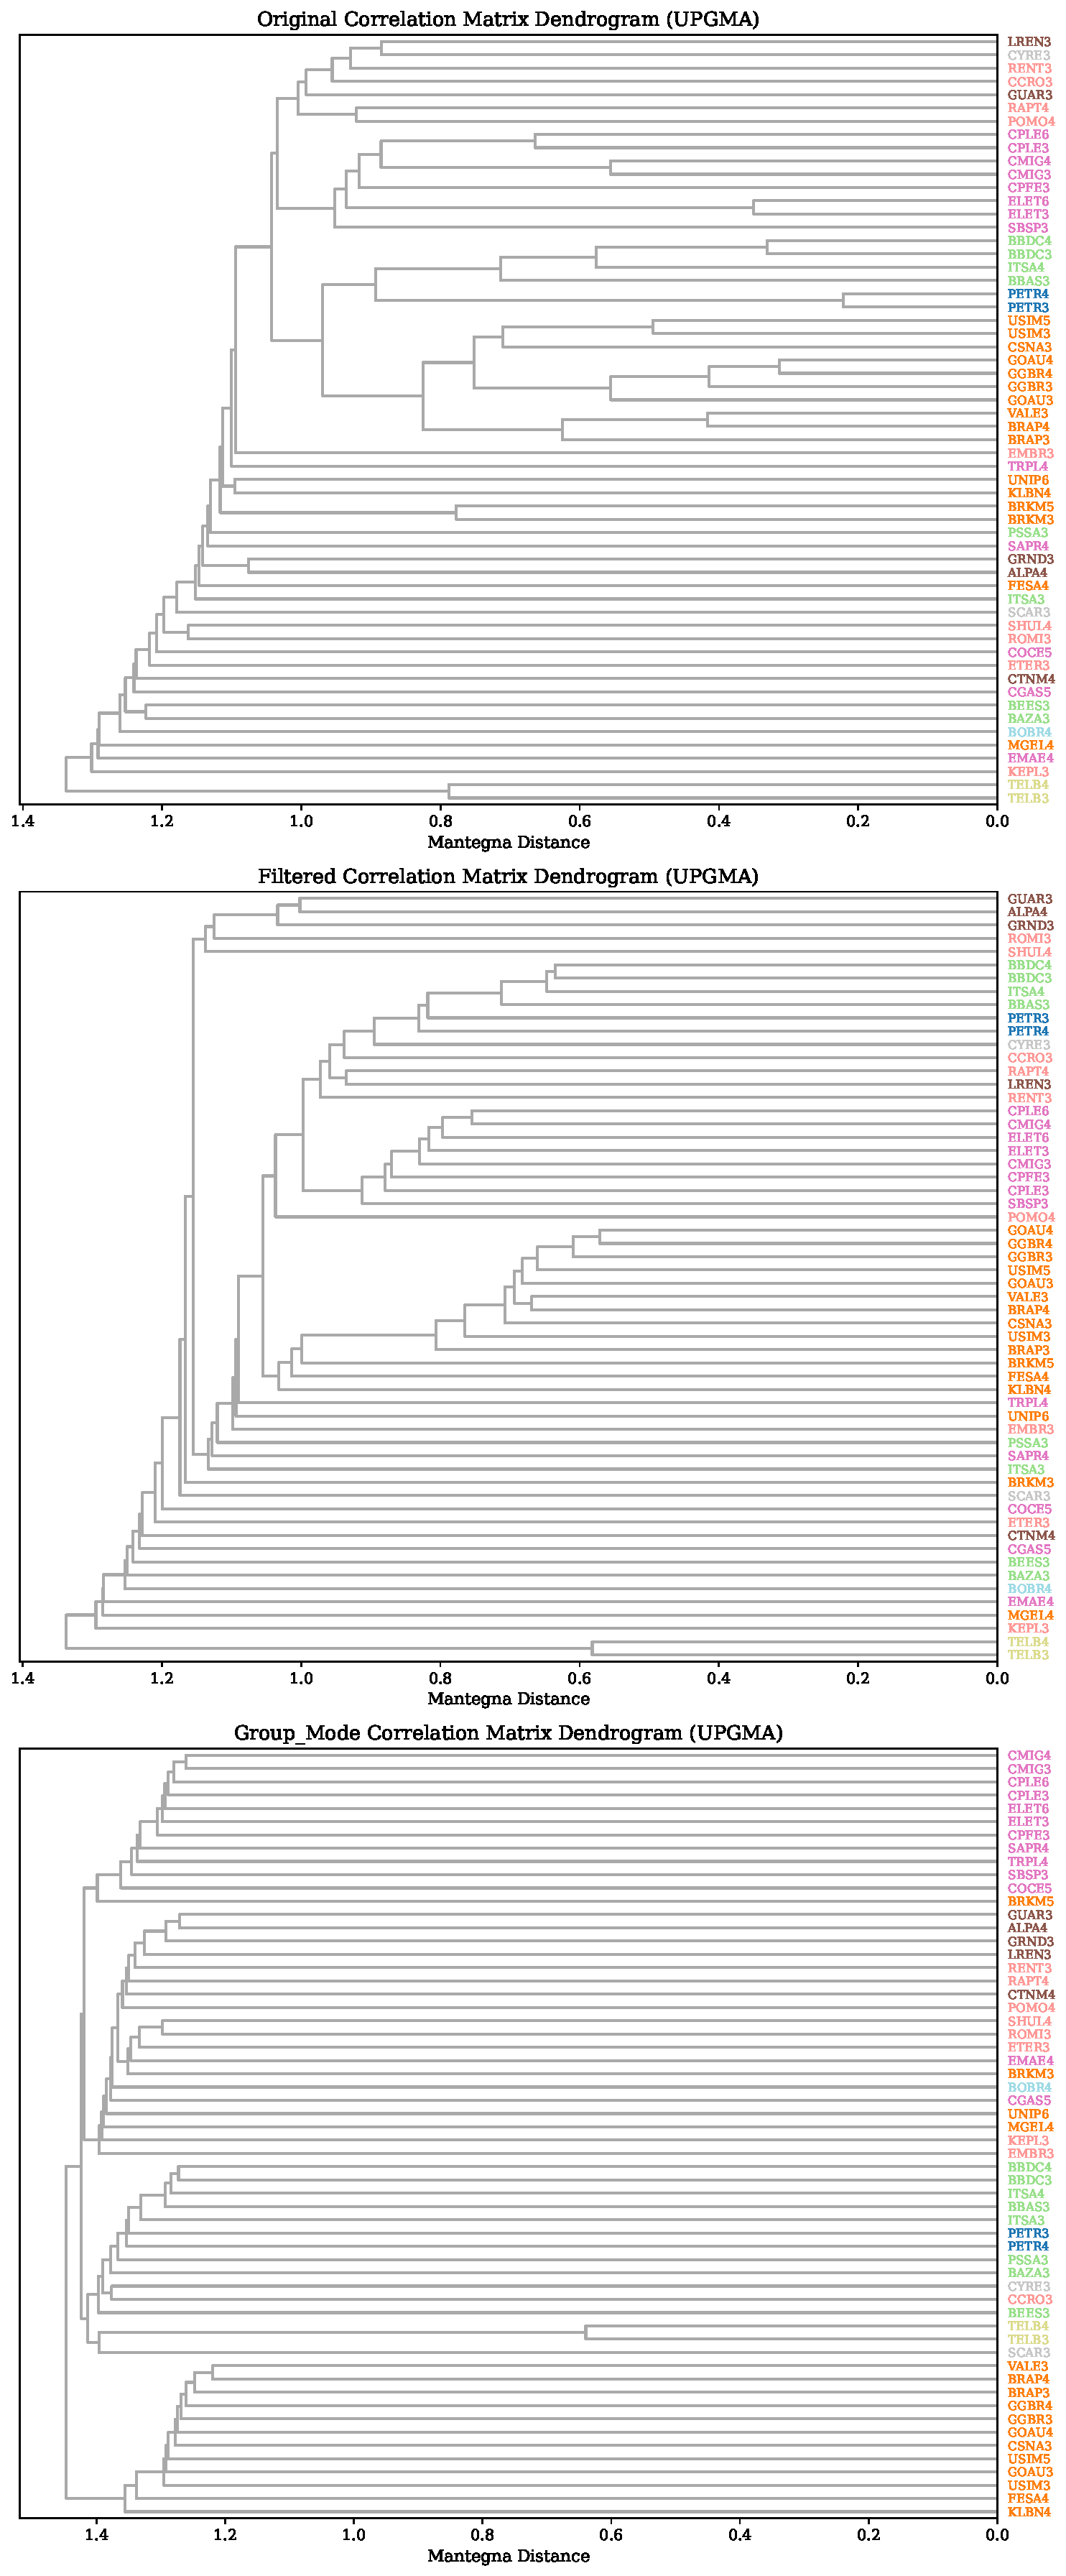
\includegraphics[width=\linewidth,height=0.90\textheight,keepaspectratio]{images/figure_9_dendrograms_comparison.pdf}
\captionof{figure}{Full dendrogram comparison for original, filtered and group-mode matrices using Mantegna distances and average linkage. The main text presents the group-mode tree only, together with the cophenetic summary.}
\label{fig:dendrograms_full_supplement}
\end{center}

\begin{center}
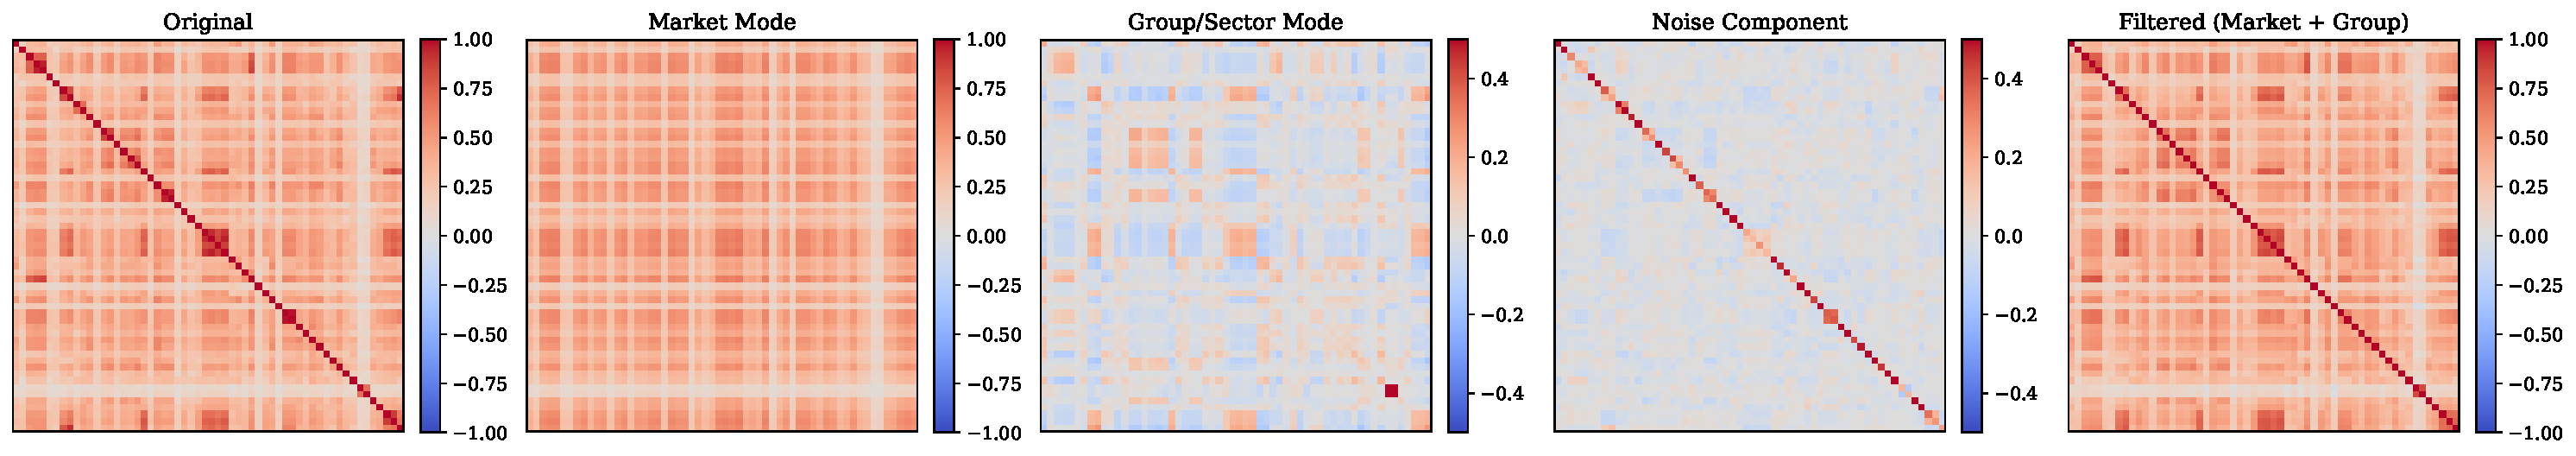
\includegraphics[width=\linewidth]{images/figure_8_rmt_filtered_matrices.pdf}
\captionof{figure}{Full RMT decomposition: original correlation, market mode, group mode, noise-compatible component and retained components. The main text presents the original and group-mode matrices at readable scale.}
\label{fig:rmt_full_components_supplement}
\end{center}

\section{Supplementary tables}
\label{app:supplementary_tables}

The following tables are generated from the computational outputs by the supplementary-table generation script. They provide the complete classified asset universe, the deterministic issuer/share-class selection, spectral loadings, null tests and asset-level forecast metrics used in the manuscript.

% Auto-generated by scripts/python/21_generate_supplementary_tables.py.
\noindent All numerical entries below are generated from the CSV files named in the captions.
\subsection{Asset universe}
\label{tab:app_universe}
\small
\begin{longtable}{llll}
\caption{Asset universe}\\
\toprule
Symbol & Company & Macro-sector & Subsector \\
\midrule
\endfirsthead
\toprule
Symbol & Company & Macro-sector & Subsector \\
\midrule
\endhead
ALPA4 & ALPARGATAS & Consumer Cyclical & Apparel and Footwear \\
BAZA3 & BANCO DA AMAZONIA & Financials & Banks \\
BBAS3 & BANCO DO BRASIL & Financials & Banks \\
BBDC3 & BRADESCO & Financials & Banks \\
BBDC4 & BRADESCO & Financials & Banks \\
BEES3 & BANESTES & Financials & Banks \\
BOBR4 & BOMBRIL & Consumer Non-Cyclical & Personal and Home Care \\
BRAP3 & BRADESPAR & Basic Materials & Mining \\
BRAP4 & BRADESPAR & Basic Materials & Mining \\
BRKM3 & BRASKEM & Basic Materials & Chemicals \\
BRKM5 & BRASKEM & Basic Materials & Chemicals \\
CCRO3 & CCR & Industrials & Transportation \\
CGAS5 & COMGAS & Utilities & Gas Utility \\
CMIG3 & CEMIG & Utilities & Electric Utility \\
CMIG4 & CEMIG & Utilities & Electric Utility \\
COCE5 & COELCE & Utilities & Electric Utility \\
CPFE3 & CPFL ENERGIA & Utilities & Electric Utility \\
CPLE3 & COPEL & Utilities & Electric Utility \\
CPLE6 & COPEL & Utilities & Electric Utility \\
CSNA3 & CSN & Basic Materials & Steel and Metallurgy \\
CTNM4 & COTEMINAS & Consumer Cyclical & Textiles \\
CYRE3 & CYRELA & Real Estate & Real Estate \\
ELET3 & ELETROBRAS & Utilities & Electric Utility \\
ELET6 & ELETROBRAS & Utilities & Electric Utility \\
EMAE4 & EMAE & Utilities & Electric Utility \\
EMBR3 & EMBRAER & Industrials & Aerospace and Defense \\
ETER3 & ETERNIT & Industrials & Construction Materials \\
FESA4 & FERBASA & Basic Materials & Steel and Metallurgy \\
GGBR3 & GERDAU & Basic Materials & Steel and Metallurgy \\
GGBR4 & GERDAU & Basic Materials & Steel and Metallurgy \\
GOAU3 & METALURGICA GERDAU & Basic Materials & Steel and Metallurgy \\
GOAU4 & METALURGICA GERDAU & Basic Materials & Steel and Metallurgy \\
GRND3 & GRENDENE & Consumer Cyclical & Apparel and Footwear \\
GUAR3 & GUARARAPES & Consumer Cyclical & Retail \\
ITSA3 & ITAUSA & Financials & Financial Services \\
ITSA4 & ITAUSA & Financials & Financial Services \\
KEPL3 & KEPLER WEBER & Industrials & Machinery and Equipment \\
KLBN4 & KLABIN & Basic Materials & Paper and Cellulose \\
LREN3 & LOJAS RENNER & Consumer Cyclical & Retail \\
MGEL4 & MANGELS & Basic Materials & Steel and Metallurgy \\
PETR3 & PETROBRAS & Oil Gas and Biofuels & Oil Gas and Biofuels \\
PETR4 & PETROBRAS & Oil Gas and Biofuels & Oil Gas and Biofuels \\
POMO4 & MARCOPOLO & Industrials & Transportation Equipment \\
PSSA3 & PORTO SEGURO & Financials & Insurance \\
RAPT4 & RANDON & Industrials & Transportation Equipment \\
RENT3 & LOCALIZA & Industrials & Transportation \\
ROMI3 & INDS ROMI & Industrials & Machinery and Equipment \\
SAPR4 & SANEPAR & Utilities & Water and Sanitation \\
SBSP3 & SABESP & Utilities & Water and Sanitation \\
SCAR3 & SAO CARLOS & Real Estate & Real Estate \\
SHUL4 & SCHULZ & Industrials & Machinery and Equipment \\
TELB3 & TELEBRAS & Telecommunications & Telecommunications \\
TELB4 & TELEBRAS & Telecommunications & Telecommunications \\
TRPL4 & ISA CTEEP & Utilities & Electric Utility \\
UNIP6 & UNIPAR & Basic Materials & Chemicals \\
USIM3 & USIMINAS & Basic Materials & Steel and Metallurgy \\
USIM5 & USIMINAS & Basic Materials & Steel and Metallurgy \\
VALE3 & VALE & Basic Materials & Mining \\
\bottomrule
\end{longtable}
\normalsize

\subsection{Issuer/share-class selection on common RMT dates}
\label{tab:app_issuer}
\small
\begin{longtable}{llrrr}
\caption{Issuer/share-class selection on common RMT dates}\\
\toprule
Company & Symbol & Common dates & Mean financial volume & Retained \\
\midrule
\endfirsthead
\toprule
Company & Symbol & Common dates & Mean financial volume & Retained \\
\midrule
\endhead
BRADESCO & BBDC3 & 1527 & 76633387 & No \\
BRADESCO & BBDC4 & 1527 & 568982596 & Yes \\
BRADESPAR & BRAP3 & 1527 & 1842568 & No \\
BRADESPAR & BRAP4 & 1527 & 86294589 & Yes \\
BRASKEM & BRKM3 & 1527 & 490990 & No \\
BRASKEM & BRKM5 & 1527 & 76536336 & Yes \\
CEMIG & CMIG3 & 1527 & 8980477 & No \\
CEMIG & CMIG4 & 1527 & 101240199 & Yes \\
COPEL & CPLE3 & 1527 & 12209461 & No \\
COPEL & CPLE6 & 1527 & 66028694 & Yes \\
ELETROBRAS & ELET3 & 1527 & 182197912 & Yes \\
ELETROBRAS & ELET6 & 1527 & 75167883 & No \\
GERDAU & GGBR3 & 1527 & 3325996 & No \\
GERDAU & GGBR4 & 1527 & 234398169 & Yes \\
ITAUSA & ITSA3 & 1527 & 3546092 & No \\
ITAUSA & ITSA4 & 1527 & 199159999 & Yes \\
METALURGICA GERDAU & GOAU3 & 1527 & 860782 & No \\
METALURGICA GERDAU & GOAU4 & 1527 & 80895038 & Yes \\
PETROBRAS & PETR3 & 1527 & 369893778 & No \\
PETROBRAS & PETR4 & 1527 & 1404540077 & Yes \\
TELEBRAS & TELB3 & 1527 & 396075 & No \\
TELEBRAS & TELB4 & 1527 & 4999879 & Yes \\
USIMINAS & USIM3 & 1527 & 12071793 & No \\
USIMINAS & USIM5 & 1527 & 171952884 & Yes \\
\bottomrule
\end{longtable}
\normalsize

\subsection{Largest absolute eigenvector loadings}
\label{tab:app_loadings}
\small
\begin{longtable}{rrllr}
\caption{Largest absolute eigenvector loadings}\\
\toprule
Rank & Eigenvalue & Symbol & Sector & $|u|$ \\
\midrule
\endfirsthead
\toprule
Rank & Eigenvalue & Symbol & Sector & $|u|$ \\
\midrule
\endhead
1 & 21.6505 & GOAU4 & Basic Materials & 0.1743 \\
1 & 21.6505 & GGBR4 & Basic Materials & 0.1713 \\
1 & 21.6505 & ITSA4 & Financials & 0.1694 \\
1 & 21.6505 & BBDC3 & Financials & 0.1676 \\
1 & 21.6505 & BBDC4 & Financials & 0.1675 \\
2 & 3.0957 & VALE3 & Basic Materials & 0.2831 \\
2 & 3.0957 & BRAP4 & Basic Materials & 0.2831 \\
2 & 3.0957 & BRAP3 & Basic Materials & 0.2507 \\
2 & 3.0957 & GGBR4 & Basic Materials & 0.2487 \\
2 & 3.0957 & GGBR3 & Basic Materials & 0.2387 \\
3 & 1.7839 & ROMI3 & Industrials & 0.2922 \\
3 & 1.7839 & SHUL4 & Industrials & 0.2903 \\
3 & 1.7839 & BBDC4 & Financials & 0.2735 \\
3 & 1.7839 & BBDC3 & Financials & 0.2689 \\
3 & 1.7839 & ITSA4 & Financials & 0.2623 \\
4 & 1.6543 & TELB3 & Telecommunications & 0.6936 \\
4 & 1.6543 & TELB4 & Telecommunications & 0.6882 \\
4 & 1.6543 & GRND3 & Consumer Cyclical & 0.0859 \\
4 & 1.6543 & ITSA3 & Financials & 0.0808 \\
4 & 1.6543 & MGEL4 & Basic Materials & 0.0694 \\
5 & 1.4835 & CMIG3 & Utilities & 0.2901 \\
5 & 1.4835 & CMIG4 & Utilities & 0.2577 \\
5 & 1.4835 & CPLE6 & Utilities & 0.2502 \\
5 & 1.4835 & CPLE3 & Utilities & 0.2265 \\
5 & 1.4835 & ALPA4 & Consumer Cyclical & 0.2129 \\
\bottomrule
\end{longtable}
\normalsize

\subsection{Circular-shift RMT null test}
\label{tab:app_rmt_null}
\small
\begin{longtable}{rrrrr}
\caption{Circular-shift RMT null test}\\
\toprule
Rank & Empirical $\lambda$ & Null 95th pct. & Exceedances & $p$ \\
\midrule
\endfirsthead
\toprule
Rank & Empirical $\lambda$ & Null 95th pct. & Exceedances & $p$ \\
\midrule
\endhead
1 & 21.6505 & 1.6882 & 0 & 0.0010 \\
2 & 3.0957 & 1.4932 & 0 & 0.0010 \\
3 & 1.7839 & 1.3889 & 0 & 0.0010 \\
4 & 1.6543 & 1.3533 & 0 & 0.0010 \\
5 & 1.4835 & 1.3295 & 0 & 0.0010 \\
6 & 1.1673 & 1.3057 & 1000 & 1.0000 \\
\bottomrule
\end{longtable}
\normalsize

\subsection{Asset-level sector-label permutation test}
\label{tab:app_sector_perm}
\small
\begin{longtable}{rrrrrr}
\caption{Asset-level sector-label permutation test}\\
\toprule
Assets & Pairs & Permutations & $\Delta_{sector}$ & Null 95th pct. & $p$ \\
\midrule
\endfirsthead
\toprule
Assets & Pairs & Permutations & $\Delta_{sector}$ & Null 95th pct. & $p$ \\
\midrule
\endhead
58 & 1653 & 10000 & 0.1184 & 0.0245 & 0.0001 \\
\bottomrule
\end{longtable}
\normalsize

\subsection{Forecast metrics by asset and horizon}
\label{tab:app_forecast}
\small
\begin{longtable}{rlllrrl}
\caption{Forecast metrics by asset and horizon}\\
\toprule
Horizon & Model & Set & Asset & MAE & RMSE & QLIKE [95\% CI] \\
\midrule
\endfirsthead
\toprule
Horizon & Model & Set & Asset & MAE & RMSE & QLIKE [95\% CI] \\
\midrule
\endhead
5 & CNN-1D & Sequence & BBDC4 & 0.0140 & 0.0224 & $-5.2596$ [$ -5.5326$, $-4.9058$] \\
5 & CNN-1D & Sequence & PETR4 & 0.0162 & 0.0245 & $-5.0712$ [$ -5.2897$, $-4.7691$] \\
5 & CNN-1D & Sequence & VALE3 & 0.0133 & 0.0171 & $-5.4093$ [$ -5.5339$, $-5.2882$] \\
5 & HAR-RV & HAR-RV & BBDC4 & 0.0154 & 0.0239 & $-5.2443$ [$ -5.5068$, $-4.8996$] \\
5 & HAR-RV & HAR-RV & PETR4 & 0.0171 & 0.0249 & $-5.1193$ [$ -5.3141$, $-4.8446$] \\
5 & HAR-RV & HAR-RV & VALE3 & 0.0144 & 0.0178 & $-5.4229$ [$ -5.5283$, $-5.3180$] \\
5 & HistGradientBoosting & Set A & BBDC4 & 0.0158 & 0.0235 & $-5.2630$ [$ -5.4942$, $-4.9894$] \\
5 & HistGradientBoosting & Set A & PETR4 & 0.0189 & 0.0273 & $-5.0398$ [$ -5.2627$, $-4.7585$] \\
5 & HistGradientBoosting & Set A & VALE3 & 0.0156 & 0.0195 & $-5.3697$ [$ -5.4807$, $-5.2602$] \\
5 & MLP & Set A & BBDC4 & 0.0134 & 0.0224 & $-5.1672$ [$ -5.4678$, $-4.7996$] \\
5 & MLP & Set A & PETR4 & 0.0153 & 0.0237 & $-5.0583$ [$ -5.2859$, $-4.7505$] \\
5 & MLP & Set A & VALE3 & 0.0126 & 0.0165 & $-5.4162$ [$ -5.5563$, $-5.2785$] \\
5 & Random Forest & Set C & BBDC4 & 0.0157 & 0.0232 & $-5.2869$ [$ -5.5162$, $-5.0082$] \\
5 & Random Forest & Set C & PETR4 & 0.0179 & 0.0262 & $-5.0658$ [$ -5.2753$, $-4.7696$] \\
5 & Random Forest & Set C & VALE3 & 0.0150 & 0.0185 & $-5.3852$ [$ -5.4908$, $-5.2695$] \\
5 & Ridge & Set C & BBDC4 & 0.0147 & 0.0233 & $-5.1358$ [$ -5.4298$, $-4.7686$] \\
5 & Ridge & Set A & BBDC4 & 0.0149 & 0.0232 & $-5.1966$ [$ -5.4669$, $-4.8556$] \\
5 & Ridge & Set C & PETR4 & 0.0158 & 0.0240 & $-5.0617$ [$ -5.2899$, $-4.7750$] \\
5 & Ridge & Set A & PETR4 & 0.0156 & 0.0239 & $-5.0801$ [$ -5.2954$, $-4.7761$] \\
5 & Ridge & Set C & VALE3 & 0.0134 & 0.0171 & $-5.4165$ [$ -5.5411$, $-5.2934$] \\
5 & Ridge & Set A & VALE3 & 0.0132 & 0.0168 & $-5.4286$ [$ -5.5435$, $-5.3098$] \\
20 & CNN-1D & Sequence & BBDC4 & 0.0224 & 0.0327 & $-3.8922$ [$ -4.1371$, $-3.5789$] \\
20 & CNN-1D & Sequence & PETR4 & 0.0220 & 0.0361 & $-3.6949$ [$ -3.9658$, $-3.3381$] \\
20 & CNN-1D & Sequence & VALE3 & 0.0186 & 0.0235 & $-4.0175$ [$ -4.1870$, $-3.8522$] \\
20 & HAR-RV & HAR-RV & BBDC4 & 0.0250 & 0.0355 & $-3.9044$ [$ -4.1309$, $-3.6263$] \\
20 & HAR-RV & HAR-RV & PETR4 & 0.0261 & 0.0393 & $-3.7300$ [$ -3.9434$, $-3.4679$] \\
20 & HAR-RV & HAR-RV & VALE3 & 0.0208 & 0.0258 & $-4.0145$ [$ -4.1623$, $-3.8753$] \\
20 & HistGradientBoosting & Set A & BBDC4 & 0.0244 & 0.0340 & $-3.9109$ [$ -4.1428$, $-3.6391$] \\
20 & HistGradientBoosting & Set A & PETR4 & 0.0299 & 0.0437 & $-3.6782$ [$ -3.8794$, $-3.4395$] \\
20 & HistGradientBoosting & Set A & VALE3 & 0.0253 & 0.0347 & $-3.9399$ [$ -4.0706$, $-3.8063$] \\
20 & MLP & Set B & BBDC4 & 0.0219 & 0.0323 & $-3.8868$ [$ -4.1323$, $-3.6029$] \\
20 & MLP & Set B & PETR4 & 0.0240 & 0.0386 & $-3.5656$ [$ -3.9185$, $-3.0508$] \\
20 & MLP & Set B & VALE3 & 0.0203 & 0.0258 & $-3.9553$ [$ -4.1344$, $-3.7615$] \\
20 & Random Forest & Set B & BBDC4 & 0.0267 & 0.0368 & $-3.8415$ [$ -4.0839$, $-3.5382$] \\
20 & Random Forest & Set B & PETR4 & 0.0320 & 0.0489 & $-3.6237$ [$ -3.8578$, $-3.3460$] \\
20 & Random Forest & Set B & VALE3 & 0.0264 & 0.0356 & $-3.9229$ [$ -4.0597$, $-3.7867$] \\
20 & Ridge & Set C & BBDC4 & 0.0241 & 0.0342 & $-3.8376$ [$ -4.0901$, $-3.5615$] \\
20 & Ridge & Set A & BBDC4 & 0.0240 & 0.0335 & $-3.9003$ [$ -4.1184$, $-3.6248$] \\
20 & Ridge & Set C & PETR4 & 0.0234 & 0.0359 & $-3.6987$ [$ -3.9358$, $-3.3962$] \\
20 & Ridge & Set A & PETR4 & 0.0225 & 0.0351 & $-3.7306$ [$ -3.9689$, $-3.4479$] \\
20 & Ridge & Set C & VALE3 & 0.0197 & 0.0245 & $-4.0097$ [$ -4.1620$, $-3.8479$] \\
20 & Ridge & Set A & VALE3 & 0.0187 & 0.0232 & $-4.0344$ [$ -4.1901$, $-3.8816$] \\
\bottomrule
\end{longtable}
\normalsize

\subsection{Issuer-panel network sensitivity on common dates}
\label{tab:app_issuer_network}
\small
\begin{longtable}{lllrrrrr}
\caption{Issuer-panel network sensitivity on common dates}\\
\toprule
Panel & Network & Matrix & $N$ & $T$ & Mean edge corr. & Same-sector & Clustering \\
\midrule
\endfirsthead
\toprule
Panel & Network & Matrix & $N$ & $T$ & Mean edge corr. & Same-sector & Clustering \\
\midrule
\endhead
full panel & MST & original & 58 & 1527 & 0.5796 & 0.7193 & 0.0000 \\
full panel & PMFG & original & 58 & 1527 & 0.5177 & 0.6012 & 0.5273 \\
full panel & MST & group-mode & 58 & 1527 & 0.1388 & 0.6316 & 0.0000 \\
full panel & PMFG & group-mode & 58 & 1527 & 0.1109 & 0.5417 & 0.6653 \\
issuer panel & MST & original & 46 & 1527 & 0.5126 & 0.6444 & 0.0000 \\
issuer panel & PMFG & original & 46 & 1527 & 0.4745 & 0.5076 & 0.5705 \\
issuer panel & MST & group-mode & 46 & 1527 & 0.0982 & 0.6000 & 0.0000 \\
issuer panel & PMFG & group-mode & 46 & 1527 & 0.0812 & 0.4621 & 0.6761 \\
\bottomrule
\end{longtable}
\normalsize

\subsection{Forecast QLIKE block-length sensitivity}
\label{tab:app_blocks}
\small
\begin{longtable}{llrrrr}
\caption{Forecast QLIKE block-length sensitivity}\\
\toprule
Horizon & Model & Set & Block & QLIKE & 95\% CI \\
\midrule
\endfirsthead
\toprule
Horizon & Model & Set & Block & QLIKE & 95\% CI \\
\midrule
\endhead
5 & HAR-RV & HAR-RV & 5 & -5.2622 & [-5.3923, -5.1118] \\
5 & HAR-RV & HAR-RV & 10 & -5.2622 & [-5.4211, -5.0715] \\
5 & HAR-RV & HAR-RV & 20 & -5.2622 & [-5.4441, -5.0591] \\
5 & Ridge & Set A & 5 & -5.2351 & [-5.3788, -5.0785] \\
5 & Ridge & Set A & 10 & -5.2351 & [-5.4009, -5.0477] \\
5 & Ridge & Set A & 20 & -5.2351 & [-5.4209, -5.0421] \\
5 & Ridge & Set B & 5 & -5.2121 & [-5.3555, -5.0459] \\
5 & Ridge & Set B & 10 & -5.2121 & [-5.3747, -5.0300] \\
5 & Ridge & Set B & 20 & -5.2121 & [-5.4011, -5.0111] \\
5 & Ridge & Set C & 5 & -5.2047 & [-5.3624, -5.0361] \\
5 & Ridge & Set C & 10 & -5.2047 & [-5.3824, -5.0211] \\
5 & Ridge & Set C & 20 & -5.2047 & [-5.3994, -4.9946] \\
20 & HAR-RV & HAR-RV & 20 & -3.8830 & [-4.0386, -3.7126] \\
20 & HAR-RV & HAR-RV & 40 & -3.8830 & [-4.0590, -3.6778] \\
20 & HAR-RV & HAR-RV & 80 & -3.8830 & [-4.0945, -3.6607] \\
20 & Ridge & Set A & 20 & -3.8884 & [-4.0514, -3.7121] \\
20 & Ridge & Set A & 40 & -3.8884 & [-4.0811, -3.6753] \\
20 & Ridge & Set A & 80 & -3.8884 & [-4.1130, -3.6508] \\
20 & Ridge & Set B & 20 & -3.8589 & [-4.0316, -3.6710] \\
20 & Ridge & Set B & 40 & -3.8589 & [-4.0699, -3.6371] \\
20 & Ridge & Set B & 80 & -3.8589 & [-4.0901, -3.6119] \\
20 & Ridge & Set C & 20 & -3.8487 & [-4.0171, -3.6669] \\
20 & Ridge & Set C & 40 & -3.8487 & [-4.0427, -3.6370] \\
20 & Ridge & Set C & 80 & -3.8487 & [-4.0704, -3.6116] \\
\bottomrule
\end{longtable}
\normalsize

\subsection{Neural-model seed sensitivity}
\label{tab:app_seeds}
\small
\begin{longtable}{llrrrrl}
\caption{Neural-model seed sensitivity}\\
\toprule
Model & Set & Horizon & Seeds & Mean QLIKE & SD & Range \\
\midrule
\endfirsthead
\toprule
Model & Set & Horizon & Seeds & Mean QLIKE & SD & Range \\
\midrule
\endhead
CNN-1D & Sequence & 5 & 5 & -5.2087 & 0.0414 & [-5.2585, -5.1659] \\
CNN-1D & Sequence & 20 & 5 & -3.8613 & 0.0072 & [-3.8695, -3.8543] \\
MLP & Set A & 5 & 5 & -5.1469 & 0.1201 & [-5.2490, -4.9479] \\
MLP & Set A & 20 & 5 & -3.6210 & 0.2801 & [-3.8887, -3.2424] \\
MLP & Set B & 5 & 5 & -4.7771 & 0.2214 & [-4.9857, -4.4077] \\
MLP & Set B & 20 & 5 & -3.6486 & 0.1037 & [-3.8026, -3.5530] \\
MLP & Set C & 5 & 5 & -4.8999 & 0.3472 & [-5.1207, -4.2906] \\
MLP & Set C & 20 & 5 & -3.7959 & 0.0559 & [-3.8656, -3.7206] \\
\bottomrule
\end{longtable}
\normalsize



\section*{Acknowledgements}

The authors gratefully acknowledge the financial support provided by the Research Support Foundation of the State of Rio Grande do Sul (FAPERGS; grants 24/2551-0001396-2 and 25/2551-0002584-2), the Brazilian National Council for Scientific and Technological Development (CNPq; grants 307416/2025-9 and 318141/2025-6), and Fesurv--UniRV.

\section*{Funding}

This research received financial support from the Research Support Foundation of the State of Rio Grande do Sul (FAPERGS; grants 24/2551-0001396-2 and 25/2551-0002584-2), the Brazilian National Council for Scientific and Technological Development (CNPq; grants 307416/2025-9 and 318141/2025-6), and Fesurv--UniRV.

\section*{Declaration of competing interest}

The authors declare that they have no known competing financial interests or personal relationships that could have appeared to influence the work reported in this paper.

\section*{Data availability}

The public BovDBv2 V1 dataset (DOI \texttt{10.7910/DVN/TMB4IG}) is distributed under CC0 1.0 and its deposited coverage ends 31 July 2024. The locally held extract used for analyses through December 2025 is not included in this package; its source-specific redistribution terms were not verified, so the public-data license is not asserted to cover it. Exact reproduction of the 2025 extension requires access to an authorized data source under its applicable terms. Analysis code, configuration files and reproducibility documentation are available in the research-software repository \cite{rmt_planar_networks_2026}.

\section*{Declaration of generative AI and AI-assisted technologies in the manuscript preparation process}

During the preparation of this work, the authors used ChatGPT for language refinement, structural organization, and code-review support. After using this tool, the authors reviewed and edited the content as needed and take full responsibility for the content of the published article.


\FloatBarrier

\printcredits

\bibliographystyle{elsarticle-num}
\bibliography{references}

\end{document}
